\documentclass[a4paper, 11.5pt]{memoir}
\usepackage{style}      % Custom style
\usepackage[CS,60,LongTitle]{masterfrontpage}
\usepackage{kantlipsum} % Dummy text
\usepackage{float}
\usepackage{tikz}
\usepackage{enumitem}
\usepackage{algorithm}
\usepackage{algpseudocode}
\newcommand*\circled[1]{\tikz[baseline=(char.base)]{
		\node[shape=circle,draw,inner sep=2pt] (char) {#1};}}

\title{A posteriori error estimation for multiple-network poroelasticity}
\author{Emilie Ødegaard}

\includeonly{
    sections/abstract,
    sections/acknowledgements,
    sections/introduction,
    sections/mathematical_background,
    sections/numerical_discretization,
    sections/error_estimation,
    sections/numerical_experiments,
    sections/summary_discussion
	%sections/appendixA,
	%sections/appendixB
}
\begin{document}
	\masterfrontpage
    \frontmatter        % Folios in Roman numerals, unnumbered chapters.
	\chapter{Abstract}

The multiple network poroelasticity equations (MPET) describes mechanical deformation and fluid flow in porous media and can be used to understand various biological processes in a physiological setting. Modeling transportation of fluid in the brain is essential to discover the underlying mechanisms that are currently being investigated concerning various neurodegenerative diseases such as Alzheimer's disease. Mathematical modeling is considered to be more accessible and less expensive than performing advanced medical tests and experiments; however numerical simulations are still prone to error, making it essential to be able to control and minimize it. Physiological frameworks often include complex geometries which may produce complex error distributions. A posteriori error estimation presents a framework to measure and control the error in specific regions of the computational domain. This thesis presents the derivation of a posteriori error estimates for MPET with two interacting fluid networks, extending the analysis from one fluid network. Numerical experiments corroborate the theoretical results. The presented a posteriori error estimates can be extended to the MPET model with an arbitrary number of networks, which is demonstrated with a computational experiment using four networks on a brain mesh with physiologically inspired parameters.


	\chapter{Acknowledgements}

First and foremost I would like to thank my supervisors, Marie E. Rognes, Kent-Andre Mardal for providing guidance and expertise throughout this Master's thesis. I am also very grateful for the time and patience that Travis Thompson has offered during the completion of the thesis; you always made time to answer my questions and motivate me to do my best. Also, I would like to thank Simula Research Laboratory for allowing me to work on an inspiring project as well as organizing an amazing summer school. Finally, I would like to thank my family and friends for the support.

	
    \tableofcontents    % Or \tableofcontents*
    %\listoffigures
    %\listoftables

    \mainmatter         % Folios in Arabic numerals, numbered chapters.

    %\appendix           % "Chapter" is renamed "Appendix"
    %\appendixpage       % Short for \part*{Appendices}
	\chapter{Introduction}
\label{chap:intro}

Poroelasticity is known to have numerous applications in biomedical engineering as well as soil mechanics and reservoir engineering \cite{coussy}. Within medical research poroelasticity can be used to simulate fluid transport through the brain \cite{tully}. The multiple network poroelasticity equations (MPET) has been introduced into geomechanics to describe mechanical deformation and fluid flow in porous media as a generalization of Biot’s theory \cite{biot, biot2}. In recent times, the MPET model has been used to better understand the influence of biomechanical risk factors associated with early stages of Alzheimer's disease \cite{guo}. The transportation of fluids and waste clearance through the brain is still not universally understood by scientists, and many questions remain unanswered \cite{iliff}. 
\\
\\
Modeling transportation of fluid in the brain is essential to discover the underlying mechanisms that are currently being investigated concerning various neurodegenerative diseases such as Alzheimer's disease \cite{bacyinski}. The current research that is being done to understand these processes is considered complex and in some cases impossible to execute, which calls for alternative methods. Mathematical simulations are often easier to perform and more cost-effective than using traditional methods such as medical experiments and advanced image processing. Complicated natural processes can be better understood through mathematical modeling, which can potentially improve treatments and the diagnosis of diseases. However, numerical simulations can be time-consuming as well as error-prone, especially when the mathematical model and the framework surrounding it is complex. Complexity is nearly unavoidable when working in a physiological framework, hence some precautions are necessary to ensure an accurate and efficient mathematical model. 
\\
\\
The presence of numerical error in mathematical approximations has been an issue ever since the technique was first introduced. Mathematical modeling relies on assumptions and simplifications about the physical world, and will inherently produce some error merely from its construction. Thus, it is important to measure this error to potentially control and minimize it. While it may in some cases be sufficient to estimate the overall accuracy of the numerical method qualitatively, it will in most cases be even more valuable to estimate the accuracy in specific regions of the computational domain. The former describes \textit{a priori} error estimators, and the latter \textit{a posteriori} error estimators, which are the two main types of error estimation techniques available \cite{verfurth96, ainsworth}. A priori error estimators give information on the overall asymptotic behavior of the error from the discretization method, while a posteriori error estimators give information on the asymptotic behavior of the error localized on each element \cite{verfurth92}. The idea is that instead of trying to minimize the total error, which is computationally expensive, an a posteriori error estimator may identify the regions where minimization is necessary. 
\\
\\
In this thesis, an in-depth derivation of the a posteriori error estimators for MPET with one and two networks is presented. A posteriori error analysis for MPET with one network has been covered in \cite{meunier, riedlbeck} and an a priori error analysis can be found in \cite{murad1, murad2, murad3}. To the best of our knowledge, an a posteriori error estimate has not yet been derived for MPET with two or more networks, with the exception of the static coupled two-network case presented by Nordbotten et al. \cite{nordbotten}. This thesis will build upon the constructed a posteriori error estimates for MPET with one network, and extend the analysis to a second network in the quasi-static formulation. The theoretical results will be evaluated using numerical experiments. 
%In addition, the a posteriori error estimators will be evaluated in a numerical implementation to determine how robust they are with varying model parameters. %MPET is computationally challenging since the physical parameters for different applications exhibit considerable variations. 
\\
\\
This thesis is organized as follows, chapter \ref{chap:math} introduces the relevant mathematical models, and chapter \ref{chap:discretization} presents the numerical methods used to solve the mathematical problems. Chapter \ref{chap:error} outlines the a posteriori error estimation techniques using a simple model problem and derives the a posteriori error estimators for MPET with one and two networks. Chapter \ref{chap:experiments} contains a presentation of the numerical experiments along with the numerical results. In chapter \ref{chap:discussion}, the results are summarized and discussed, and provides conclusions and directions for future work.
\\
\\
The numerical experiments was done using FEniCS \cite{fenics} (version 2018.1.0) in Docker \cite{docker} (version 18.03.1). The code can be found here: \url{https://github.com/emilieodegaard/master}

\newpage
\section{Notation}
The following notation will be used throughout this thesis.
\\
\\
\begin{tabular}{lll}
                  & \textbf{General symbols} & \\[3pt]
    $\Omega $   & The domain of interest, an open subset of $\R^n$ &\\ [3pt]
    $\partial\Omega$   & Exterior boundary of $\Omega$ &\\[3pt]
    $u$  & Displacement &\\[3pt]
    $p$  & Pressure &\\[3pt]
    $\nabla \cdot $  & Divergence  & \\[3pt]
    $\nabla $ & Gradient  & \\[3pt]
    $\Delta$  & Laplace operator &\\[3pt]
                 & \textbf{Model parameters} & \\[3pt]
    $\alpha$  & Biot-Willis coefficient &  \\[3pt]
    $\mu$      & Lamé parameter & Pa $\cdot$ s  \\[3pt]
    $\lambda$  & Lamé parameter & m$^2$ s$^{-1}$  \\[3pt]
    $Q^{-1}$    & Compressibility  & Pa \\[3pt]
    $c$    & := $Q^{-1}$, Storage coefficient & Pa$^{-1}$\\[3pt]
 	$\kappa$   & Permeability parameter  & m$^{2}$\\[3pt]
    $K$   & := $\kappa / \mu$ Mobility parameter  & m$^{2}$ Pa$^{-1}$ s$^{-1}$\\[3pt]
    $\xi$     & Transfer parameter  & Pa$^{-1}$ s$^{-1}$\\[3pt]
                  & \textbf{Function spaces} & \\[3pt]
    $\R$ & Real numbers &  \\[3pt]
    $\N$ & Natural numbers & \\[3pt]
    $C^0(\Omega)$  & Set of continuous functions & \\[3pt]
    $C^{\infty}(\Omega)$  & Set of smooth functions & \\[3pt]
    $C^k(\Omega)$  & Set of functions with continuous derivatives up to order $k$ & \\[3pt]
    $C^k_0(\Omega)$  & Subset of $C_k$ of functions with compact support &\\[3pt]
    $L^2(\Omega)$ & Space of square-integrable functions &\\[3pt]
    $L^2_0(\Omega)$  & Subset of $L^2$ of functions with compact support &\\[3pt]
    $H^m(\Omega)$ & Sobolev space of $L^2$ functions with square-integrable \\
    $H^m_0(\Omega)$  & Subset of $H^m$ of functions with compact support &\\[3pt]
    &  derivatives up to order m &\\[3pt]
    $H^{-1}(\Omega)$  & Dual space of $H^1(\Omega)$ &\\[3pt]
    & \textbf{The finite element method} & \\[3pt]
    $\langle \cdot, \cdot \rangle$  & $L^2$-inner product over $\Omega$ &\\[3pt]
    $\partial \Omega_D$  & Part of the boundary $\partial \Omega $
                                         with Dirichlet boundary conditions  &\\[3pt]
    $\mathcal{P}_q(T)$ &  Space of polynomials of total
                       degree $\leq q$ over T &\\[3pt]
    $P_q$   & Lagrange element of degree $q$ &\\[3pt]
\end{tabular}
\newpage
\begin{tabular}{lll}
    & \textbf{Finite element partition} & \\[3pt]
    $\mathcal{T}_h$   & Partition of $\Omega$ &\\[3pt]
    $h$   & Maximum diameter of the elements in $\mathcal{T}_h$ &\\[3pt]
    $T$   & Element in $\mathcal{T}_h$ &\\[3pt]
    $E$   & Face or edge of $T$ in $\mathcal{T}_h$ &\\[3pt]
    $\mathcal{E}_T$   & Faces of $T$ &\\[3pt]
    $\mathcal{E}_\Omega$   & Faces having at least one endpoint in the interior of $\Omega$ &\\[3pt]
    $\mathcal{E}_{\partial\Omega}$   & Faces contained in the boundary &\\[3pt]
     $\mathcal{E}_{\partial\Omega_D}$   & Faces contained in the Dirichlet boundary &\\[3pt]
    $\omega_T$   & Elements sharing a face with $T$ &\\[3pt]
    $\tilde{\omega}_T$  & Elements sharing a vertex with $T$ &\\[3pt]
    $\omega_E$   & Elements sharing adjacent to $E$ &\\[3pt]
    $\tilde{\omega}_E$  & Elements sharing a vertex with $E$ &\\[3pt]
	$\psi_T$  & Element bubble function &\\[3pt]
	$\psi_E$  & Face bubble function &\\[3pt]
    $C_{\mathcal{T}}$   & Shape parameter of $\mathcal{T}_h$ &\\[3pt]
 \end{tabular}

\section{Mathematical preliminaries}
\label{section:prelim}
This section presents the mathematical theory and results necessary for the derivation of the a posteriori error estimates. All theory is compiled from \cite{verfurth13} with the exception of \ref{def:trace} which is from \cite{riviere}.

\begin{definition}[\textbf{$L^P$-space}]\label{def:LP_space}
Let $\Omega$ be an open subset of $\mathbb{R}^n$. For $1\leq p \leq \infty$, $L^p(\Omega)$ is defined as
\begin{equation}
L^p(\Omega) = \{u \in \Omega : (\int_\Omega |u|^p dx)^\frac{1}{p} < \infty\}
\end{equation}
with the corresponding norm $\|u\|_{L^p(\Omega)} = (\smallint_\Omega |u|^p dx)^\frac{1}{p}$
\end{definition}

\begin{definition}[\textbf{Weak derivative}]\label{def:weak_derivative}
Let $\Omega$ be an open subset of $\mathbb{R}^n$. Assume $u,v \in L^1_{loc}(\Omega)$ and let $\alpha=(\alpha_1, ..., \alpha_n)$ denote a multi-index. Then $v$ is referred to as the $\alpha^{th}$ weak derivative of $u$ if
\begin{equation}
\int_\Omega u D^\alpha \phi dx = (-1)^{|\alpha|}\int_\Omega v \phi dx
\end{equation}
for all $\phi \in C_0^\infty(\Omega)$, where $D^\alpha \phi$ is defined as, 
\begin{equation}
D^\alpha \phi = \frac{\partial^{|\alpha|}\phi}{\partial^{\alpha_1}x_1 \cdots \partial^{\alpha_n}x_n} 
\end{equation}
\end{definition}
\begin{remark}
$L^1_{loc}(\Omega)$ denotes all locally integrable functions for the open set $\Omega$.
\end{remark}

\begin{definition}[\textbf{Sobolev space}]\label{def:sobolev}
Let $\Omega$ be an open subset of $\mathbb{R}^n$. For a nonnegative integer $m$ where $\alpha=(\alpha_1, ..., \alpha_n)$ denotes a multi-index, the Sobolev space $H^m(\Omega)$ is defined as
\begin{equation}
H^m(\Omega) = \{u \in \Omega : (\sum_{|\alpha|\leq m} \int_\Omega |D^\alpha u|^2 dx)^\frac{1}{2} < \infty \}
\end{equation}
with the corresponding norm $\|u\|_{H^m(\Omega)}=(\sum_{|\alpha|\leq m} \int_\Omega |D^\alpha u|^2 dx)^\frac{1}{2}$
\end{definition}

\begin{definition}[\textbf{$H^1$-norm and semi-norm}]\label{def:semi_norm}
The space $H^1(\Omega)$ is defined by the norm, 
\begin{equation}
\|u\|_{H^1(\Omega)} = (\int_\Omega u^2 + (\nabla u)^2 dx)^\frac{1}{2}
\end{equation}
and the semi-norm,
\begin{equation}
|u|_{H^1(\Omega)} = (\int_\Omega (\nabla u)^2 dx)^\frac{1}{2}
\end{equation}
The semi-norm is defined on the subspace $H_0^1(\Omega)$.
\end{definition}

\begin{theorem}[\textbf{Galerkin orthogonality}]\label{def:galerkin}
For a given bilinear from $a(\cdot, \cdot)$ the following Galerkin orthogonality holds
\begin{align}
a(u-u_h, v_h) = 0 \hspace{0.5cm} \forall v_h \in V_h
\end{align}
where $V_h$ is the discrete subspace of $V$.
\end{theorem}

\begin{theorem}[\textbf{Support}]\label{def:support}
Given a continuous function $u : \mathbb{R}^d \rightarrow \mathbb{R}$, the support is denoted by 
\begin{align*}
\textnormal{supp} \, u = \overline{\{x \in \mathbb{R}^d : \phi(x) \neq 0\}}
\end{align*}
\end{theorem}
\begin{remark} All functions satisfying the condition "supp $\phi \subset \Omega$" vanish on the boundary of $\Omega$ as well as all their derivatives. This is because the condition is non-trivial as supp $\phi$ is closed and $\Omega$ is open. 
\end{remark}

\begin{theorem}[\textbf{Poincaré inequality}]\label{def:poincare}
For all $u \in H^1(\Omega)$ with $\int_\Omega u = 0$, 
\begin{equation}
\|u \|_{H^0} \leq c_\Omega |u|_{H^1}
\end{equation}
where $c_\Omega$ depends on the domain $\Omega$. 
\end{theorem}

\begin{theorem}[\textbf{Friedrich inequality}] \label{def:friedrich}
For all $u \in H^1_D(\Omega)$, 
\begin{equation}
\|u \|_{H^0} \leq c'_\Omega |u|_{H^1}
\end{equation}
where $c'_\Omega$ depends on the domain $\Omega$. 
\end{theorem}

\begin{theorem} [\textbf{Young's inequality}]\label{def:young}
For nonnegative real numbers $a$ and $b$, where $p$ and $q$ are positive real numbers such that $\frac{1}{p} + \frac{1}{q} = 1$, then
\begin{equation}
ab \leq \frac{a^p}{p} + \frac{b^q }{q}
\end{equation}
\end{theorem}

\begin{theorem} [\textbf{Approximation by interpolation}]\label{def:approx}
There exists an interpolation operator $\pi_h : H^t(\Omega) \rightarrow V_h$, where $V_h$ is a piecewise polynomial field of order $t-1$ with the property that for any $u \in H^t(\Omega)$
\begin{equation}
\|u - \pi_h u \|_{H^m} \leq C h^{t-m}\| u\|_{H^t}
\end{equation}
\end{theorem}

\begin{theorem} [\textbf{Quasi-interpolation operator}]\label{def:interpol}
There exists a quasi-interpolation operator $I_h : L^1(\Omega) \rightarrow V_h$ with the property that for any $u \in H^1_D(\Omega)$ for all elements $T\in \mathcal{T}$,
\begin{align*}
& \, \|u - I_h u \|_{L^2(T)} \leq c_1 h_T \|u\|_{H^1(\tilde{\omega}_T)},\\
& \, \|u - I_h u \|_{L^2(\partial T)} \leq c_2 h_T^{\frac{1}{2}} \|u\|_{H^1(\tilde{\omega}_T)}
\end{align*}
where $\tilde{\omega}_T$ denotes the set of all elements that share at least a vertex with $T$. 
\end{theorem}
\begin{remark}
The quasi-operator does not interpolate a given function at the vertices. 
\end{remark}

\begin{definition}[\textbf{Element bubble function}] \label{def:bubble_est}
For every element $T \in \mathcal{T}$ the \textit{element bubble function} $\psi_T$ has the following properties,
\begin{align*}
\psi_T(x) \in  [0,1] \quad & \,\forall x \in T \\
\psi_T(x) =  0 \quad & \, \forall x \notin T \\
\max_{x \in T} \psi_T(x) = 1 
\end{align*}
The following inverse estimates holds for all polynomials $\phi \subset \mathbb{P}^k$,
\begin{align*}
c_{I1,k}\|\phi \|_T \leq & \, \|\psi_T^{\frac{1}{2}}\phi\|_T \\
\|\nabla(\psi_T\phi) \|_T \leq & \, c_{I2,k}H_T^{-1}\|\phi\|_T
\end{align*}
\end{definition}

\begin{definition}[\textbf{Face/edge bubble function}] \label{def:bubble_est_edge}
For every face $E \in \mathcal{E}$ the \textit{face bubble function } $\psi_E$ fulfills,
\begin{align*}
\psi_E(x) \in [0,1] \quad & \, \forall x \in \omega_E \\
\psi_E(x) = 0 \quad  & \, \forall x \notin \omega_E \\
\max_{x \in \omega_E} \psi_E(x) = 1 
\end{align*}
The inverse estimates holds for all polynomials $\phi \subset \mathbb{P}^k$,
\begin{align*}
c_{I3,k}\|\phi \|_E \leq & \, \|\psi_E^{\frac{1}{2}}\phi\|_E \\
\|\nabla(\psi_E\phi) \|_{\omega_E} \leq & \, c_{I4,k}H_E^{-\frac{1}{2}}\|\phi\|_E \\
\|\psi_E\phi \|_{\omega_E} \leq & \, c_{I5,k}H_E^{\frac{1}{2}}\|\phi\|_E 
\end{align*}
where $\omega_E$ is the union of all elements that share $E$.
\end{definition}

\begin{definition}[\textbf{Jump function}] \label{def:jump}
For each edge $E \in \mathcal{E}$, the jump across $E$ in the direction $\mathbf{n}_E$ is defined as,
\begin{equation}
\mathbb{J}_E(\mathbf{n}_E \cdot u) = \llbracket \mathbf{n}_E\cdot u \rrbracket =  \mathbf{n}^+ \cdot u ^+ - \mathbf{n}^- \cdot u ^-
\end{equation}
\end{definition}

\begin{theorem}[\textbf{Trace inequalities}]\label{def:trace}
For every element $T$ with face or edge $E$ and all $u \in \mathbb{P}^k$ the following holds,
\begin{align*}
\|u\|_{L^2(E)} \leq c_{T1} h_T^{-\frac{1}{2}}\|u\|_{L^2(T)} \quad \forall u \in E \subset \partial T \\
\|\nabla u \cdot \mathbf{n}\|_{L^2(E)} \leq c_{T2} h_T^{-\frac{1}{2}}\|\nabla u\|_{L^2(T)} \quad \forall u \in E \subset \partial T
\end{align*}
where $c_{T1}$ and $c_{T2}$ are constants depending on the size of the shape parameter. 
\end{theorem}
	\chapter{Mathematical models} 
\label{chap:math}
The multiple-network poroelasticity equations (MPET) describe the relationship between flow and deformation in a poroelastic medium with interconnected fluid networks. The model was first introduced as an application in geosciences to model storage reservoirs \cite{aifantis1979, aifantis1980, berryman2002}. Since porous media includes biological tissues, Tully and Ventikos \cite{tully} suggests that the equations can be used to model interacting biological fluids and tissues in a physiological setting, which is also the primary motivation behind this thesis. 
\\
\\
This chapter outlines the mathematical models used in the thesis. Section \ref{section:mpet} presents the MPET model and is mainly based on the work of Bai et al. \cite{bai}. Section \ref{section:poisson} presents the Poisson model, which is used to introduce the main mathematical methods in chapter \ref{chap:error}. The Poisson model is presumed to be the most fundamental PDE and is often used as a simple model problem before tackling more complex PDEs, which is also the purpose it serves here. 

\section{Multiple-network poroelasticity model (MPET)} 
\label{section:mpet}
We consider a linearly elastic and porous medium $\Omega$ saturated by a nearly incompressible and viscous  fluid. The multiple-network poroelasticity model (MPET) is defined as
\\
\begin{align} \label{eq:mpet1}
\rho \ddot{u} - \nabla \cdot (\sigma^{\ast}) + \displaystyle\sum_a \alpha_a \nabla p_a = 0  \\ 
- \nabla \cdot K_a \rho_a  \ddot{u} +  c_a\dot{p_a} + \alpha_a \nabla \cdot\dot{u} - \nabla \cdot K_a \nabla p_a + S_a = g_a  \label{eq:mpet2}
\end{align}
\\
where we for each network $a=1,2,\dots, A$ seek the displacement $u = u(x,t)$ and the pressure $p_a = p_a(x,t)$ for $x \in \Omega$ and time $t$ such that \eqref{eq:mpet1}-\eqref{eq:mpet2} is fulfilled. The equations arises from a balance of mass and momentum in an elastic porous medium permeated by fluid networks.
\\
\\
We denote $\dot{u}$ as the time derivative of $u$. $\rho$ represents the density of the elastic tissue matrix and $\alpha_a$ the Biot-Willis coefficient. $K_a$ denotes the mobility of the medium where $K_a = \kappa_a/\mu_a$ and $\kappa_a$ is defined as the permeability and $\mu_a$ the viscosity. $\rho_a$ denotes the density and $c_a$ the compressibility in network $a$. $\dot{s}_{b \rightarrow a} $ represents the nonnegative exchange coefficients from network $b$ to $a$ and $g_a$ is defined as any sources/sinks in network $a$. 
\\
\\
Assuming that the medium deforms elastically and anisotropically, a fourth order stiffness tensor $C$ defines the stress tensor $\sigma^*$ by Hooke's law:
\begin{align}
\sigma^*(u) = 2\mu \, \epsilon(u) + \lambda \textnormal{tr}(\epsilon(u)) I
\end{align}
where $\epsilon(u)$ is the symmetric gradient, 
\begin{align}
\epsilon(u) = \frac{1}{2}\left( \nabla(u) + \nabla(u^T)\right)
\end{align}
The trace of $u$, $\textnormal{tr}(u)$ is defined as the sum of the elements on the main diagonal of $u$. $I$ is the identity matrix. 
\\
\\
The transfer terms $S_a$ quantifies the transfer out of network $a$ into the other fluid networks. If a hydrostatic pressure gradient powers the the rate of transfer from network $b$ to $a$, the exchange coefficients can be described as:
\begin{align}
S_a(\vec{p}) = S_a(p_1, ...,p_A) = \displaystyle\sum_{b=1}^A \xi_{b \rightarrow a}(p_a - p_b)
\end{align}
where $\xi_{b \rightarrow a}$ is a transfer coefficient from network $b$ to $a$. We assume that the transfer coeffiecient are nonnegative, i.e. $\xi_{j \to i} \geq 0$ for $1 \leq i,j \leq A$. In addition, we assume $\xi_{i \to i} = 0$ for all $i \in \{1, ..., A\}$ and $\xi_{i \to j} = \xi_{j \to i}$ for all $i,j \in \{1, ..., A\}$. We set $c_a^{-1} = \infty$ and $\alpha_a = 1 $ for all $a$ if all networks are assumed incompressible. 
\\
\\
%%%%%%%%%%%%%%%%%%%%%%% SIMPLIFIED MODEL %%%%%%%%%%%%%%%%%%%%%%
In this thesis we will ignore the acceleration terms, so that our model is reduced to: 
\\
\begin{align} \label{eq:mpet_simple1}
- \nabla \cdot (\sigma^{\ast}) + \displaystyle\sum_a \alpha_a \nabla p_a = 0
\\
 c_a\dot{p_a} + \alpha_a \nabla \cdot\dot{u} - \nabla \cdot K_a \nabla p_a + S_a = g_a \label{eq:mpet_simple2}
\end{align}
This is known as the quasi-static formulation of the Barenblatt-Biot model, which is appropriate when the application does not involve shear or compression waves, e.g. systolic pulsation \cite{tully}. 
\\
\\
%%%%%%%%%%%%%%%%%%%%%%% BIOT %%%%%%%%%%%%%%%%%%%%%%%
When we are working with one network, \eqref{eq:mpet_simple1}-\eqref{eq:mpet_simple2} is reduced to what is known as the  \textit{Biot model} \cite{biot}. This model studies a medium assumed to contain only one fluid network permeating it. 
\begin{align} \label{eq:biot1}
- \nabla \cdot(\sigma^{\ast}) +  \alpha \nabla p = f \\
c\dot{p} + \alpha \nabla \cdot\dot{u} - \nabla \cdot K \nabla p = g \label{eq:biot2}
\end{align}
Here $f$ denotes any external forces and $g$ the source/sink in the network. An analysis of the existence and uniqueness of the strong and weak solutions of the Biot model has been derived in \cite{showalter, zenisek}. Note that since there is only one network, there exists no transfer and thus, $S_a=0$.
\\
\\
%%%%%%%%%%%%%%%%%%%%%%% BIOT-BARENBLATT %%%%%%%%%%%%%%%%%%%%%%%
The \textit{Barenblatt-Biot model} \cite{Barenblatt1960,Barenblatt1963, elsworth, berryman1995} extends the Biot model \eqref{eq:biot1}-\eqref{eq:biot2} to another network, i.e. $A=2$. Here the poroelastic medium is assumed to have a dual permeability, which results in a system with two diffusion equations representing the two networks. These are coupled by an exchange term which describes the potential difference between the fluids in the two fluid components. The quasi-static formulation of the Barenblatt-Biot model is,
%The problem then becomes: find $u = u(x,t)$ and the pressure $p_1 = p_1(x,t)$, $p_2 = p_2(x,t)$ for $x \in \Omega$ and time $t$ such that
\begin{align} \label{math_model:mpet2_u}
- \nabla \cdot(\sigma^{\ast}) +  \alpha_1 \nabla p_1 +  \alpha_2 \nabla p_2 = f \\
c_1\dot{p}_1 + \alpha_1 \nabla \cdot \dot{u} - \nabla \cdot (K_1 \nabla p_1) + \xi_{2\to 1}(p_1-p_2) = g_1 \label{math_model:mpet2_p1}\\
c_2\dot{p}_2 + \alpha_2 \nabla \cdot \dot{u} - \nabla \cdot(K_2 \nabla p_2) + \xi_{1\to 2}(p_2-p_1) = g_2 \label{math_model:mpet2_p2}
\end{align}
where $u$ is the displacement and $p_1$ and $p_2$ are the fluid potentials in the respective fluid components. $f$ denotes any external forces and $g_1$ and $g_2$ sources/sinks in networks $1$ and $2$, respectively. We also denote $\xi_{2\to 1}$ as the transfer coefficient from network 1 to network 2, and vice verca for $\xi_{1\to 2}$. The existence of solution for the Barenblatt-Biot model can be found in \cite{showalter, showalter2002}.

\section{Poisson model} \label{section:poisson}
The Poisson equation is an elliptic PDE which describes a potential field caused by a charge density \cite{bitsadze}. We assume homogeneous Dirichlet boundary conditions. Then the Poisson problem is defined as,
\\
\begin{align} \label{eq:poisson_strong_form}
- \Delta \, u = & \, f \hspace{0.5cm} \textnormal{in} \hspace{0.2cm} \Omega \\
u = & \, 0 \hspace{0.5cm} \textnormal{on} \hspace{0.2cm}\Gamma_D
\end{align}
As with the poroelasticity equations, $f$ denotes any external forces. We know that there exists a unique solution for the Poisson model, see e.g. \cite{evans}.
	\chapter{Numerical discretization}
\label{chap:discretization}
There are several equations where the exact solution is either unknown or not explicitly available \cite{evans}. In such cases, a numerical approximation is sought. The finite element method is a numerical method to approximate solutions of partial differential equations. The general idea of this method is to divide the problem into a set of smaller and simpler problems, called elements, and find an approximated solution on each element for then to merge all the approximations to find the global solution. The first step is to define a weak form of the PDE followed by a discretization of the physical domain. Then, a finite discretized space of functions is constructed related to the discretization. Finally, the weak form is approximated in the finite element space using a Galerkin method where the problem is reduced to a system of algebraic equations. 
\\
\\
This chapter derives the discretization of the mathematical models presented in chapter \ref{chap:math}. The methods are widely used and can be found in several introductory books on the finite element method, see, e.g. \cite{brenner, ern, gatica}. Section \ref{section:disc_mpet} presents the discretization of the MPET model, where the spatial discretization follows the temporal discretization. Section \ref{disc_poisson} derives the discretization for the Poisson model. In addition, a priori error estimates for both mathematical models are provided in section \ref{section:a_priori}.

\section{Discretization of MPET} \label{section:disc_mpet}
In this thesis, we will assume that the data is smooth enough for a strong solution to exist, which includes the boundary and initial conditions as well as the source terms. In addition, the problem is a so-called \textit{mixed problem}, as the unknown variables are the displacement $u$ and the pressure $p$. These need to be approximated in different finite element spaces, giving a mixed variational formulation. The multiple-network poroelasticity equations (MPET) consists of both temporal and spatial derivatives, so the following sections outline the discretization first in time and then in space. 

\subsection{Temporal discretization of MPET}
We use a Backward-Euler time discretization with $t\in (0,T]$ and assume $\tau_n = t^n - t^{n-1}$ for $0 \leq n \leq N$. The problem then becomes: given $u^{n-1}$ and $p_a^{n-1}$, find $u^n$ and $p_a^n$ at all steps $n = 0, ..., N$ for every network $a=1,..A$ such that,
\begin{align} \label{temp_disc_mpet1}
- \nabla \cdot \sigma^{\ast^n}(u^n) + \displaystyle\sum_a \alpha_a \nabla p_a^n = f^n \\
c_a\left(\frac{p_a^n - p_a^{n-1}}{\tau_n} \right) + \alpha_a \nabla \cdot\left(\frac{u^n - u^{n-1}}{\tau_n}  \right) - \nabla \cdot K_a \nabla p_a^n + S_a(\vec{p}^n) = g_a^n \label{temp_disc_mpet2}
\end{align}
where,
\begin{equation} \label{S_a}
S_a(p_1^n, ..., p_A^n) = \displaystyle\sum_{b=1}^A \xi_{b \rightarrow a}(p^n_a - p^n_b)
\end{equation}
\\
\\
To accommodate the finite element formulation from a strict PDE-problem to several smaller problems, we need to take away some of the conditions on the unknown solutions, $u$ and $\vec{p} = (p_1,..,p_A)$. To do this, we introduce a weak formulation of the equation, which allows for the equation to not hold absolutely but instead hold in relation to a test function in a chosen function space. The idea is that if the test function is sufficiently smooth, the requirements made on the unknown solution may be reduced by doing integration by parts on the terms with higher-order derivatives. 
\\
\\
In order to find the weak form of the temporal discretization, we introduce \textit{trial functions} $u\in V$, $p_a \in Q$ for each network $a=1,..A$ and their respective \textit{test functions} $v \in \hat{V}$, $q_a \in \hat{Q}$. The test functions are typically assumed to be independent of time. Furthermore, their respective trial and test spaces are defined as,
\begin{align} 
V:= &\{v \in H^1(\Omega; \R^d) \, | \, v = \bar{u} \,\, \text{on} \, \, \partial \Omega\}, \hspace{0.5cm} 
\hat{V} :=  \{v \in V \, | \, v = 0 \,\, \text{on} \, \, \partial \Omega \} \\
Q:= &\{q_a \in L^2(\Omega; \R^d) \, | \, q_a = \bar{q_a} \,\, \text{on} \, \, \partial \Omega\}, \, \,
\hat{Q} := \{q_a \in Q \, | \, q_a = 0 \,\, \text{on} \, \, \partial \Omega\}
\end{align}
where $V,\hat{V} \subseteq L^2(\Omega)$ and $Q,\hat{Q} \subseteq H^1(\Omega)$ and $\bar{u}$ and $\bar{q_a}$ are some given functions. 
\\
\\ 
Boundary conditions can be prescribed by considering two partitions of the boundary: one for the displacement field and the other for the pressure field. For the sake of simplicity, a Dirichlet condition is enforced on the displacement and the pressure everywhere for this thesis. The following boundary conditions will be used,
\begin{align}
u =  u_e \,\, & \, \text{on} \, \, \partial \Omega \, \, \, \forall t\in(0,T]\\
p_a = p_{a_e} \,\, & \,\text{on} \, \, \partial \Omega \, \, \forall t\in(0,T]
\end{align}
\\
Let $\langle\cdot, \cdot \rangle$ denote the $L^2$ inner product over $\Omega$. All test functions are required to vanish where the boundary is known, and the weak form of the problem thus becomes: find $u^n \in V$, $p_a^n \in Q_a$ for each network $a=1,..A$ such that, 
\\
\begin{align} \label{mpet_disc1}
\langle \sigma^*(u^n), \nabla v \rangle - \displaystyle\sum_a \langle \alpha_a p_a^n ,\nabla \cdot v \rangle = &\, \langle f^n , v \rangle \\
\langle c_a p_a^{n} + \alpha_a \nabla \cdot \,u^n + \tau_n S_a(p^n),  q_a \rangle + K_a \tau_n\langle \nabla p_a, \nabla q_a\rangle  = & \, \langle G_a^n, q_a\rangle \label{mpet_disc2}
\end{align}
for all $v \in \hat{V}$ and $q_a \in \hat{Q}$, where,
\begin{align} \label{G_source}
G_a^n = \tau_n g_a^n + c_a p_a^{n-1} + \alpha_a \nabla \cdot \, u^{n-1}
\end{align}
\\
We note that as $\sigma^*(u)$ is a symmetric tensor, the inner product $\langle \sigma^*(u^n), \nabla  v^n \rangle$ will result in $\langle \sigma^*(u^n), \epsilon(v) \rangle$ as the asymmetric part of the product vanishes.
\subsection{Spatial discretization of MPET}
Given a mesh $\mathcal{T}_h$, we define discrete spaces $V_h$ and $Q_h$ which are assumed to be finite-dimensional subspaces of $V$ and $Q$, respectively. Here $h$ is defined as the size of the elements in the mesh $\mathcal{T}_h$. We use Taylor-Hood elements to approximate the displacement and pressure, i.e. continuous piecewise second order polynomials for the displacement and continuous piecewise linears for the pressure. Let $0 = t_0 < t_1 <...< t_N = T$ be a sequence of discrete time steps for all $n\in\{1,..., N \}$.  
\\
\\
The weak form of the spatial discretization is then: given $u_h^{n-1}$ and $p_{a_h}^{n-1}$, find $u_h^n \in \hat{V}_h$ and $p_{a_h}^n \in \hat{Q}_h$ with $x\in \Omega \subset \R^n$ such that for all $n\in\{1,..., N \}$,
\begin{align} \label{mpet_fem1}
\langle C \epsilon(u_h^n), \epsilon(v_h) \rangle - \sum_a \langle \alpha_a p_{a_h}^n ,\nabla \cdot v_h \rangle = & \langle f_h^n , v_h \rangle  \\
\langle c_a p_{a_h}^{n} + \alpha_a \nabla \cdot u_h^n + \tau_n S_a(\vec{p_h}^n),  q_{a_h} \rangle + K_a \tau_n \langle \nabla p_{a_h}, \nabla q_{a_h}\rangle = & \langle G_{a_h}^n, q_{a_h}\rangle  \label{mpet_fem2}
\end{align}
for all $v_h \in \hat{V_h}$ and $q_{a_h} \in \hat{Q_h}$, where $G_{a_h}^n$ is defined as,
\begin{equation} \label{Gh_source}
G_{a_h}^n = \tau_n g_{a_h}^n + c_a p_{a_h}^{n-1} + \alpha_a \nabla \cdot \, u_h^{n-1}
\end{equation}
\subsubsection{Bilinear form} \label{section:num_disc_bilinear}
It is practical to work with the bilinear form of the discrete problem when deriving the a posteriori error estimates which will be outlined in chapter \ref{chap:error}. Hence, we need to establish a framework for this. 
\\
\\
Let $V$ and $Q$ be two Hilbert spaces equipped with bilinear forms $a(\cdot, \cdot)$ and $b(\cdot, \cdot)$ respectively. Furthermore, we assume that the bilinear forms are symmetric, continuous and coercive. These forms will induce the norms $\|\cdot\|_a$, $\|\cdot\|_b$ respectively. Let $V'$ and $Q'$ be the respective dual space of $V$ and $Q$ with inner product $\langle \cdot, \cdot \rangle_a$ and norm $\| \cdot\|_{a'} = \sup{0 \neq v \in V} \|\langle \cdot, v \rangle_a\| / \|v\|_a$ (resp. for $Q'$).  
\\ 
\\
The bilinear form of the discrete problem is then, for each network $a=1,...,A$, find $u_h^n \in \hat{V}_h$ and $p_{a_h}^n \in \hat{Q}_h$ such that for all $n\in\{0,..., N \}$,
\begin{align} \label{bilinear}
a(u_h^n, v_h) - \sum_a b_a(v_h, p_{a_h}^n) = & \, \langle f_h^n, v_h \rangle \\
c_a(\partial_t p_{a_h}^n, q_{a_h}) + b_a( \partial_t u_h^n, q_{a_h}) + d_a(p_{a_h}^n, q_{a_h}) + \langle S_a(\vec{p_h}^n), q_{a_h}\rangle= & \, \langle g_{a_h}^n, q_{a_h} \rangle 
\end{align}
\\
for all $v_h \in \hat{V}_h$ and all $q_{a_h} \in \hat{Q}_h$, where,
\begin{align*}
a(u_h^n, v_h) = \langle \sigma^*(u_h^n), \nabla \, v_h \rangle, \hspace{0.5cm}
& b_a(v_h, p_h^n) =  \alpha_a \langle p_{a_h}^n ,\nabla \cdot \, v_h \rangle \\
c_a(\partial_t p_h^n, q_h) = c_a \langle \partial_t p_{a_h}^{n},  q_{a_h} \rangle, \hspace{0.5cm} 
& d_a(p_h^n, q_h) = K_a \langle \nabla \,p_{a_h}, \nabla\, q_{a_h}\rangle
\end{align*}
and $S_a(\vec{p_h}^n)$ is defined as in \eqref{S_a}. 
\\
\\
Note that we did not integrate by parts the second term in \eqref{temp_disc_mpet2} in \eqref{bilinear}. The reason for this is that the second term in \eqref{temp_disc_mpet1} and the second term in \eqref{temp_disc_mpet2} are very similar in their structure which gives an advantage in the analysis; they are "adjoints" of each other. 
\\
\\
It will also be practical to define the following bilinear map for the transfer terms summed over all networks $a$, i.e. $T : [L^2(\Omega)]^A \times [L^2(\Omega)]^A \to \mathbb{R}$,
\begin{equation} \label{T_transfer}
T(\vec{p},\vec{q}) = \frac{1}{2}\sum_{a,b=1}^A \xi_{b\rightarrow a} \langle p_{a} - p_{b}, q_a - q_b\rangle
\end{equation}
with the associated semi-norm, 
\begin{equation}
| \cdot |_T = \sqrt{T(\cdot, \cdot) }
\end{equation}
By the symmetry of the transfer coefficients $\xi_{b \to a}$, \eqref{T_transfer} can be written as, 
\begin{equation} \label{T(p,q)}
T(\vec{p},q) = \sum_{a=1}^A \langle S_a(p), q_a\rangle
\end{equation}
In light of this, we now define a norm on $[L^2(\Omega)]^A$, 
\begin{equation} \label{d_hat_norm}
\| \cdot\|_{\hat{d}} := \sum_{a=1}^A \|\cdot \|_d + \| \cdot \|_T
\end{equation}
Note that $\| \cdot\|_{\hat{d}} = \|\cdot \|_d$ when $A=1$. Also, note that each mass conservation equation in the MPET model contains pieces of the $\hat{d}$-norm and the full $\hat{d}$-norm is only obtained in the analysis when summing the full set of mass conservation equations together. That is, it will not be applied at a single network level. In addition, $\| \cdot\|_{\hat{d}}$ is symmetric since $T(\cdot,\cdot)$ and $d(\cdot,\cdot)$ are symmetric. It is important to point out that the $\hat{d}$-norm serves the purpose of making the analysis simple and easily extendable to the analysis done for the single network case, which will become clear in chapter \ref{chap:error}.
\begin{remark}
Please note that we use $c_a(\cdot, \cdot)$ to define a bilinear form and $c_a$ to be the storage coefficient for network $a$.
\end{remark} 

\section{Discretization of Poisson} \label{disc_poisson}
The strong form of the Poisson model is given in \eqref{eq:poisson_strong_form}, which has the variational form: find $u \in V$ such that
\begin{align} \label{poisson_disc}
\langle \nabla u , \nabla v  \rangle = \langle f, v  \rangle \hspace{0.5cm} \forall v \in V
\end{align}
where,
\begin{align}
V = \{u \in H^1(\Omega) : u = 0 \,\,\, \textnormal{on} \,\,\, \Gamma_D \}
\end{align}
Note that $V$ is also known as $H^1_0(\Omega)$. 
\\
\\
Let $V_h \subset V$ be a finite dimensional subspace of $V$. Then the corresponding discrete variational problem is: find $u_h \in V_h$ such that,
\begin{equation} \label{eq:poisson_variational}
\langle \nabla \, u_h, \nabla \, v_h \rangle = \langle f, v_h  \rangle \hspace{0.5cm} \forall v_h \in V_h
\end{equation}

\section{A priori error estimates} \label{section:a_priori}
In this section, a priori error estimates for the MPET problem (A=1,2) and the Poisson problem will be derived. The a priori error estimates provide an estimate for the expected convergence rates of the norm of the error. This is necessary since computing the convergence rates will validate our results and ensure that we see what we should according to the mathematical theory. A more detailed explanation of convergence rate is presented in section \ref{section:convergence_rate}. The a priori error estimates for the Biot model has been analyzed in \cite{meunier} and an analysis of the a priori error estimates for the Barenblatt-Biot model can be found in \cite{boal}.
\\
\begin{definition}[\textbf{A priori error estimate (MPET, A=1)}]
Let $u\in V$ and $p \in Q$ be the solution to \eqref{mpet_disc1}-\eqref{mpet_disc2} with A=1, and let $u_h \in V_h$ and $p_h \in Q_h$ be the solution to \eqref{mpet_fem1}-\eqref{mpet_fem2} with A=1, discretized with Taylor-Hood elements. Then, the following estimate holds,
\begin{equation*}
\|u - u_h \|_{H^1} + \|p - p_h \|_{L^2} \leq Ch^2\|u \|_3 + Dh^2\|p \|_2
\end{equation*}
for sufficiently smooth solutions. This follows from \eqref{def:approx} using $m=1$ and $t=3$ for $\|u - u_h \|_{H^1}$ and $m=0$ and $t=2$ for $\|p - p_h \|_{L^2}$. The estimate states that the $H^1$-error for the displacement and the $L^2$-error for the pressure is expected to be of at least second order. 
\end{definition}

\begin{definition}[\textbf{A priori estimate (MPET, A=2)}]
Let $u\in V$ and $(p_1, p_2) \in( Q \times Q)$ be the solution to \eqref{mpet_disc1}-\eqref{mpet_disc2} with A=2, and let $u_h \in V_h$ and $(p_{1h}, p_{2h}) \in (Q_h \times Q_h)$ be the solution to \eqref{mpet_fem1}-\eqref{mpet_fem2} with A=2, discretized with Taylor-Hood elements. Then, the following estimate holds,
\begin{equation*}
\|u - u_h \|_{H^1} + \|p_1 - p_1h \|_{L^2} + \|p_2 - p_2h \|_{L^2} \leq Ch^2\|u \|_3 + Dh^2\|p_1 \|_2 + E h^2\|p_2 \|_2
\end{equation*}
for sufficiently smooth solutions. This follows from \eqref{def:approx} using $m=1$ and $t=3$ for $\|u - u_h \|_{H^1}$ and $m=0$ and $t=2$ for $\|p_1 - p_1h \|_{L^2}$ and $\|p_2 - p_2h \|_{L^2}$. The estimate states that the $H^1$-error for the displacement and the $L^2$-error for the pressures is expected to be of at least second order. 
\end{definition}

\begin{definition}[\textbf{A priori estimate (Poisson)}]
Let $u\in V$ be the solution to \eqref{poisson_disc} and let $u_h \in V_h$ be the solution to \eqref{eq:poisson_variational}. Then, the following estimates holds,
\begin{equation*}
\|u - u_h\|_{H^1} \leq Ch^2\|u \|_3
\end{equation*} 
\begin{equation*}
\|u - u_h\|_{L^2} \leq Ch\|u \|_2
\end{equation*}
for sufficiently smooth solutions. This follows from \eqref{def:approx} with $m=1$ and $t=2$ for $\|u - u_h\|_{H^1}$ and $m=0$ and $t=1$ for $\|u - u_h\|_{L^2}$. The estimate states that the $H^1$-error for $u$ is expected to be of at least third order, wile the $L^2$-error for $u$ is expected to be of at least second order.
\end{definition}


	\chapter{A posteriori error estimation}
\label{chap:error}
This chapter presents the main concepts and theory used in constructing the a posteriori error estimates for the mathematical models introduced in chapter \ref{chap:math}. A discussion on a posteriori error estimates for linear, elliptic and parabolic problems can be found in \cite{ainsworth, verfurth92, bangerth, babuska78b}. To demonstrate the fundamental theory of a posteriori error estimation, we first start with a simple model problem: the Poisson model, and then expand upon that to derive the a posteriori error estimates for MPET.
\\
\\
The primary purpose of a posteriori error estimation is to gain information about the size of the error in the spatial and temporal distribution of the problem domain. This allows us to identify the regions where the error is high and where the error is low. On the grid-points where the error is high, we wish to perform refinement to obtain higher accuracy. On the grid-points where the error is low, we wish to either keep them that way or try with a higher mesh resolution to ensure a minimal number of grid-points. The idea is that instead of trying to minimize the total error with a priori error estimation, which is computationally expensive, an a posteriori error estimator identifies the regions where minimization is necessary.
\\
\\
The general form of an error estimator usually looks like, 
\begin{equation} \label{error_est}
\|u - u_h \| \leq C(h)
\end{equation}
where $u$ is the exact solution, $u_h$ the numerical approximated solution, $h$ is a discretization parameter and $C(h)$ is some function of $h$. For the finite element method, $u$ is the solution of the PDE, $u_h$ is the finite element solution for a mesh with element size $h$. The estimate aims to minimize the error by decreasing the size of $h$. 
We are, in other words, interested in constructing the right-hand side of \eqref{error_est}, which will be the goal for the following sections. 
\\
\\
For the error estimator to be effective and perform optimally, it needs to fulfill a set of requirements \cite{verfurth92}. First, the error estimate should be accurate in the sense that the predicted error is close to the actual, unknown error. Second, the error estimated needs to be asymptotically correct. This means that they should tend to zero at the same rate as the actual error with a smaller discretization parameter. Ideally, the error estimator should yield guaranteed upper and lower bounds of the true error. The estimator should also be computationally simple, where the error estimate is inexpensive to compute when measuring the total computation time of the numerical solving. Lastly, the implementation should allow for an adaptive refinement process. 
\\
\\
Refinement can in many ways be viewed as the main goal of a posteriori error estimation procedures. To carry out refinement, we need the following:
\begin{enumerate}[noitemsep]
\item A discretization method.
\item A solver for the discrete problems.
\item An error estimator which furnishes the a posteriori error estimate. 
\item A refinement strategy.
\end{enumerate}
The first two points were covered in chapter \ref{chap:discretization}. The current chapter will focus on the third point: constructing the a posteriori error estimates for our model. Note that this thesis will not focus on point four, the refinement strategy. We will instead direct the reader to e.g. \cite{mitchell, eriksson} and chapter 2 in \cite{verfurth13}. 
\\
\\
There are different types of a posteriori error estimators, including residual estimates, hierarchical basis error estimates, H(div)-lifting, averaging methods and auxiliary problem solutions \cite{verfurth13}. This thesis will focus on the first type of error estimator: \textit{residual estimates}. The basic idea of residual error estimates is to decompose the global residual into a number of local problems on small element partitions \cite{babuska78a}. To construct the residual estimate, we first find the $L^2$-representation of the residual and separate it into element and edge residuals. Next, we find upper and lower bounds on the residuals and end with showing that the norm of the error can be bounded from above and below by the residuals. This will be the procedure for our derivation of the a posteriori error estimates for the mathematical models presented in chapter \ref{chap:math}. 
\\
\\
This chapter will first derive residual-based a posteriori error estimates for the Poisson model and the MPET model with one network, which are estimators that have already been derived in \cite{verfurth96} and \cite{meunier}, respectively. Using the techniques from these derivations, we then present the a posteriori error estimator for the MPET model with two networks. This chapter is organized as follows, section \ref{section:error_poisson} outlines the fundamental theory in deriving a posteriori error estimates with the Poisson model as an example. Section \ref{section:error_mpet} derives the a posteriori error estimators for the MPET model with one network, and then extending that analysis to two networks. 

\section{Poisson model} \label{section:error_poisson}
To illustrate some of the necessary conditions needed for an efficient error estimator we start with a simple example: the Poisson equation with homogeneous Dirichlet boundary conditions as presented in \eqref{eq:poisson_strong_form}.  
\\
\\
The derivation of the residual estimators will occur in the following way: we first split the residual into elements and edges. We then insert the element residuals into the strong form of the differential equation. The edge residuals are derived via integration by parts on each element and consists of the jumps between each element of the trace operator. The edge residuals connect the strong and weak form of the differential equation. The residual estimates yield upper and lower bound for the error of the numerical discrete solution up to multiplicative constants. The upper bounds are global on the computational domain, whereas the lower bounds are local on each element and its neighbors. The following analysis is based on a posteriori error estimation methods inspired by \cite{verfurth13, neittaanmaki, repin}.
\\
\\
We let $\langle .,.\rangle$ denote the $L^2$ inner product on $\Omega$ where $\Omega$ is a connected, bounded domain in $\R^2$ with boundary $\partial \Omega$. We assume $f$ to be a square-integrable function on $\Omega$. Using the variational form of the Poisson equation \eqref{eq:poisson_variational} from chapter \ref{chap:discretization}, we know that every $v \in V$ satisfies,
\begin{equation} \label{eq:poisson_disc}
\langle \nabla u, \nabla v \rangle = \langle f,v \rangle 
\end{equation}
Observe that by adding and substracting $u_h$ inside $\nabla u$ in \eqref{eq:poisson_disc} we have,
\begin{equation} \label{eq:poisson_residuala}
\langle \nabla (u-u_h), \nabla v \rangle =  \langle f,v \rangle - \langle \nabla u_h, \nabla v \rangle
\end{equation}
For every $v \in V$ we define the residual, 
\begin{equation} \label{eq:poisson_residual}
\langle R(u_h), v \rangle :=  \langle f,v \rangle - \langle \nabla u_h, \nabla v \rangle
\end{equation}
Then \eqref{eq:poisson_residuala} implies that, 
\begin{equation} \label{eq:poisson_residualb}
\langle R(u_h), v \rangle =  \langle \nabla (u-u_h), \nabla v \rangle
\end{equation}
Observe that we may bound the norm of the error using the definition of the semi-norm in $H^1$,
\begin{align}
\|\nabla(u-u_h) \|_{H^0(\Omega)} = |u-u_h|_{H^1(\Omega)} \leq \|u-u_h\|_{H^1(\Omega)}
\end{align}
Using Friedrich \eqref{def:friedrich} and Cauchy-Schwarz inequality on \eqref{eq:poisson_residualb} we then have,
\begin{equation} \label{eq:poisson_sup}
\sup_{\substack{v\in V \\ \| \nabla v\|=1}} \langle R, v \rangle \leq \| \nabla (u-u_h) \|_{L^2(\Omega)}  \leq \| u-u_h \|_{H^1(\Omega)} \leq \sqrt{1+c^2_\Omega} \sup_{\substack{v\in V \\ \| \nabla v\|=1}}\langle R, v \rangle
\end{equation}
We may thus conclude that the norm of the error $\| u-u_h \|_{H^1(\Omega)}$ may be bounded up to a multiplicative constant, from above and below by the norm of the residual. Our next step is therefore to find these upper and lower bounds on the error. To do this, we start by separating the residuals elementwise and edgewise to localize the error on each element.

\subsection{Element and edge residuals}
We let $T$ denote the element and $E$ the edge/face of a mesh $\mathcal{T}$. Using integration by parts on the formulation for the residual \eqref{eq:poisson_residuala}, we have for every $v \in V$,
\begin{align} \label{poisson_el_edge}
\int_\Omega \nabla(u-u_h) \nabla v = & \, \int_\Omega fv - \int_\Omega \nabla u_h \nabla v \\ 
= & \,  \displaystyle\int_\Omega fv + \displaystyle\sum_{T \in \mathcal{T} } \left( \displaystyle\int_T \Delta u_h v - \displaystyle\int_{\partial T} \mathbf{n}_T \cdot \nabla u_h v\right) \notag\\ 
= & \, \displaystyle\sum_{T \in \mathcal{T}} \displaystyle\int_T (f + \Delta u_h) \,v - \displaystyle\sum_{E \in \mathcal{E}} \displaystyle\int_E \mathbb{J}_E(\mathbf{n}_E \cdot \nabla u_h) \, v  \notag
\end{align}
Recall that $\langle \nabla(u-u_h), \nabla v \rangle = \langle R(u_h), v \rangle$ of \eqref{eq:poisson_residualb}. Inserting this into the left-hand side of \eqref{poisson_el_edge}, we have the following representation of the residual,
\begin{equation} \label{eq:res_L2}
\int_\Omega R(u_h) v = \, \, \displaystyle\sum_{T \in \mathcal{T}} \displaystyle\int_T R_T(u_h)\, v  + \displaystyle\sum_{E \in  \mathcal{E}} \displaystyle\int_E R_E(u_h) \, v
\end{equation}
where we define the \textit{element residual}, 
\begin{equation} \label{eq:element_res}
R_T(u_h) = f + \Delta u_h \quad T \in \mathcal{T} 
\end{equation}
and the \textit{edge residuals} as,
\begin{equation} \label{eq:edge_res}
R_E(u_h) = \begin{cases} 
	- \mathbb{J}_E(\mathbf{n}_E \cdot \nabla u_h) & \quad  E \in \mathcal{E}_\Omega \\
     0 & \quad E \in \mathcal{E}_{\Gamma_D} \\
\end{cases}
\end{equation}
Note that we have used that the exterior unit normal in the negative direction is defined as $\mathbf{n}^- = -\mathbf{n}$. This yields, 
\begin{align}
\displaystyle\sum_{T \in \mathcal{T}} \displaystyle\int_{\partial T}\mathbf{n}_T \cdot \nabla u_h v = & \, \displaystyle\sum_{E \in \mathcal{E}} \displaystyle\int_E \mathbf{n}^+ \nabla u_h^+ v + \displaystyle\int_E \mathbf{n}^- \nabla u_h^- v \\
= & \, \displaystyle\sum_{E \in \mathcal{E}} \displaystyle\int_E \mathbf{n} \nabla u_h^+ v + \displaystyle\int_E (-\mathbf{n}) \nabla u_h^- v\notag\\
= & \, \displaystyle\sum_{E \in \mathcal{E}} \displaystyle\int_E \left(\nabla u_h^+ - \nabla u_h^- \right)\cdot \mathbf{n} \, v \notag\\
= & \, \displaystyle\sum_{E \in \mathcal{E}} \displaystyle\int_E \mathbb{J}_E(\mathbf{n}_E \cdot \nabla u_h) \, v \notag
\end{align} 
The last equality is deduced from the definition of the jump function \ref{def:jump}. 
\\
\subsection{Upper bound} \label{poisson_up_bd_section}
We start by fixing $w\in V$ and let $w_h = I_h w$ where $I_h$ is the quasi-interpolation operator \eqref{def:interpol} from section \ref{section:prelim}. Recall that due to the Galerkin orthogonality we have equality when using the test functions $w$ and $w-w_h$. We thus have,
\\
\begin{align} \label{poisson:up_bd1}
\int_\Omega \nabla(u-u_h) \nabla v = & \, \displaystyle\sum_{T \in \mathcal{T}} \displaystyle\int_T R_T(u_h)\, w  + \displaystyle\sum_{E \in \mathcal{E}} \displaystyle\int_E R_E(u_h) \, w  \\ 
= & \, \displaystyle\sum_{T \in \mathcal{T}} \displaystyle\int_T R_T(u_h)\, (w-w_h)  + \displaystyle\sum_{E \in \mathcal{E}} \displaystyle\int_E R_E(u_h) \, (w-w_h) \notag
\end{align}
\\
Inserting the test function $w_h$ into \eqref{poisson:up_bd1} and using the Cauchy-Schwartz inequality yields, 
\begin{align} \label{poisson:up_bd4a}
\langle \nabla(u-u_h), \nabla w \rangle \leq  & \displaystyle\sum_{T \in \mathcal{T}} \| R_T(u_h)\|_T \|(w-I_h w)\|_T  \\ 
& + \displaystyle\sum_{E \in \mathcal{E}} \| R_E(u_h) \|_E \|(w-I_h w)\|_E \notag
\end{align}
\\
We use the quasi-interpolation operator \ref{def:interpol} on \eqref{poisson:up_bd4a} to get, 
\begin{align} \label{poisson:up_bd5a}
\langle \nabla(u-u_h), \nabla w \rangle \leq & \, \displaystyle\sum_{T \in \mathcal{T}} \| R_T(u_h)\|_T c_1 h_T \|w\|_{H^1(\tilde{\omega}_T)} \\
+ & \, \displaystyle\sum_{E \in \mathcal{E}} \| R_E(u_h) \|_E c_2 h_E^{\frac{1}{2}} \|w\|_{H^1(\tilde{\omega}_E)} \notag
\end{align}
Finally, using the Cauchy-Schwarz inequality for sums on \eqref{poisson:up_bd5a} we get,
\begin{align} \label{poisson:up_bd6a}
\langle \nabla(u-u_h), \nabla w \rangle \leq  \max\{c_1, c_2\}\bigl\{& \, \sum_{T \in \mathcal{T}} h_T^2\| R_T(u_h)\|^2_T \\
& \quad + \sum_{E \in \mathcal{E}} h_E\| R_E(u_h) \|^2_E \bigr\}^\frac{1}{2}  \notag \\
& \, \cdot \bigl\{\sum_{T \in \mathcal{T}} \|w\|^2_{H^1(\tilde{\omega}_T)} + \sum_{E \in \mathcal{E}}\|w\|^2_{H^1(\tilde{\omega}_E)}\bigr\}^\frac{1}{2} \notag
\end{align}
\\
\\
We observe that due to the shape regularity of $\mathcal{T}$, we have for some constant $c$, 
\begin{equation} \label{poisson:up_bd2}
\bigl\{ \displaystyle\sum_{T \in \mathcal{T}} \|w\|^2_{H^1(\tilde{\omega}_T)} + \displaystyle\sum_{E \in \mathcal{E}} \|w\|^2_{H^1(\tilde{\omega}_E)} \bigr\}^\frac{1}{2} \leq c \| w\|_{H^1}
\end{equation}
\\
Using \eqref{poisson:up_bd2} on \eqref{poisson:up_bd6a} we then have, 
\begin{align} \label{poisson:up_bd3}
\langle \nabla(u-u_h), \nabla w \rangle \leq  \max\{c_1, c_2\}\bigl\{\sum_{T \in \mathcal{T}} h_T^2\| R_T(u_h)\|^2_T \\
+ \sum_{E \in \mathcal{E}} h_E\| R_E(u_h) \|^2_E \bigr\}^\frac{1}{2} c \| w\|_{H^1} \notag
\end{align}
\\
We wish to use \eqref{eq:poisson_sup} in order to get the final upper bound on the norm of the error. Using \eqref{eq:poisson_sup} on \eqref{poisson:up_bd3} yields the upper bound,
\begin{equation} \label{eq:poisson_a_posteriori0}
\| u - u_h \|_{H^1(\Omega)} \leq c^* \bigl\{ \displaystyle\sum_{T \in \mathcal{T}} h_T^2\| R_T\|^2_T + \displaystyle\sum_{E \in \mathcal{E}} h_E\| R_E \|^2_E \bigr\}^\frac{1}{2}
\end{equation}
where the constant $c^*$ is defined as
\begin{align*}
c^* = \max \{c_1, c_2\} c \sqrt{1+c_\Omega^2}
\end{align*}
Note we may use \eqref{eq:poisson_a_posteriori0} as an a posteriori error estimator since it only depends on the numerical solution $u_h$ and the known source term $f$. We summarize the result below.
\subsection{Preliminary residual error estimator}
We define a preliminary error estimator $\eta_p$ for the POisson model with elements $T$ and edges $E$, where $R_T$ and $R_E$ are defined as in \eqref{eq:element_res} and \eqref{eq:edge_res},
\begin{equation} \label{eq:poisson_eta1}
\eta_p = \bigl\{ \displaystyle\sum_{T \in \mathcal{T}} h_T^2\| R_T\|^2_T + \displaystyle\sum_{E \in \mathcal{E}} h_E\| R_E \|^2_E \bigr\}^\frac{1}{2}
\end{equation}
such that for a constant $c^*$ we have,
\begin{equation} \label{eq:poisson_a_posteriori1}
\| u - u_h \|_{H^1(\Omega)} \leq c^* \eta_p
\end{equation}
\\
In order to maintain an efficient error estimator, a lower bound on the error is also needed. The next section outlines the derivation of the lower bound for \eqref{eq:poisson_variational}, which is mainly based on the works of Verfürth \cite{verfurth13, verfurth92}.
\\ 
%%%%%%%%%%%%%%%%%%%%%%%%% LOWER BOUND %%%%%%%%%%%%%%%%%%%%%%%%%
\subsection{Lower bound} \label{section:poisson_lower bound}
We fix an arbitrary element $\tilde{T}$, and let $w_{\tilde{T}} = (f_T + \Delta u_h) \psi_{\tilde{T}}$ be a test function where $f_T = \frac{1}{|T|}\int_T f \mathrm{d}x$ and $\psi_{\tilde{T}}$ is a bubble function. We insert $w_{\tilde{T}}$ into \eqref{eq:res_L2} to get,
\begin{equation} \label{lowbd1}
\langle R, w_{\tilde{T}} \rangle = \displaystyle\sum_{T \in \mathcal{T}}\displaystyle\int_T R_T(u_h)\, w_{\tilde{T}} + \displaystyle\sum_{E \in \mathcal{E}}\displaystyle\int_E R_E(u_h) w_{\tilde{T}} 
\end{equation}
\\
Note that the support of $\psi_{\tilde{T}}$ is $\tilde{T}$, which implies that \eqref{lowbd1} is,
\begin{equation} \label{eq:lowbd2}
\langle R, w_{\tilde{T}} \rangle  =  \displaystyle\int_T R_T(u_h)w_{\tilde{T}}
\end{equation}
\\
Recalling again that $\langle R, v \rangle = \langle \nabla (u-u_h) \nabla v\rangle$ of \eqref{eq:poisson_residualb}, we insert this into the left-hand side of \eqref{eq:lowbd2},
\begin{align} \label{eq:lowbd3}
\langle \nabla (u-u_h) \nabla w_{\tilde{T}} \rangle = & \, \displaystyle\int_T R_T(u_h)w_{\tilde{T}} \\ 
= & \, \displaystyle\int_T (f+\Delta u_h) w_{\tilde{T}}  \notag 
\end{align}
\\
Note that this equality requires $w_{\tilde{T}} \in V_h$. Next, we add $\int_T (f_T - f) w_T$ to both sides of \eqref{eq:lowbd3} and insert $w_{\tilde{T}}$ into the integral on the right-hand side,
\begin{equation} \label{eq:lowbd4}
\displaystyle\int_T \nabla (u-u_h) \nabla w_{\tilde{T}} + \displaystyle\int_T (f_T - f) w_{\tilde{T}} = \, \displaystyle\int_T (f_T+\Delta u_h)^2 \psi_{\tilde{T}}
\end{equation}
\\
\\
We now inspect the three terms in \eqref{eq:lowbd4} separately starting with the first term on the left-hand side. For practical reasons, we now let $\tilde{T} = T$. This gives, 
\begin{align}\label{eq:lowbd5}
\displaystyle\int_T \nabla (u-u_h) \nabla w_T \leq & \, \| \nabla (u-u_h)\|_T\| \nabla w_T \|_T \\
= & \, \| \nabla (u-u_h)\|_T\| \nabla((f_T + \Delta u_h)\psi) \|_T \notag\\
\leq & \, \| \nabla (u-u_h)\|_T c_{I2}h_T^{-1} \|f_T + \Delta u_h)\|_T  \notag
\end{align}
\\
For the second term of \eqref{eq:lowbd4} we have
\begin{align}\label{eq:lowbd6}
\displaystyle\int_T (f_T-f) w_T \leq & \, \| f_T-f\|_T \|w_T\|_T \\
\leq & \, \| f_T-f\|_T \|f_T + \Delta u_h\|_T   \notag
\end{align}
To arrive at \eqref{eq:lowbd5} and \eqref{eq:lowbd6} we have used the Cauchy-Schwartz inequality and the inverse estimates for bubble functions \eqref{def:bubble_est}. For the term on the right-hand side we use the second inverse estimate for bubble functions to get,
\begin{align} \label{eq:lowbd7}
\displaystyle\int_T (f_T+\nabla u_h)^2 \psi_T \, \geq \, c_{I1}^2 \| f_T + \Delta u_h\|_T^2
\end{align}
\\
Inserting \eqref{eq:lowbd5}, \eqref{eq:lowbd6} and \eqref{eq:lowbd7} into \eqref{eq:lowbd4}, we get the lower bound for an element $T$,
\begin{align} \label{eq:llowbd8}
h_T \| f_T + \Delta u_h\|_T \leq c_{I1}^{-2} \left(c_{I2}\|\nabla(u-u_h) \|_T + h_T \|f-f_T\|_T \right)
\end{align}
\\
We will use this inequality later on, so we rename the constants so that $c_1 = c_{I1}^{-2}c_{I2}$ and $c_2 = c_{I1}^{-2}$. This gives, 
\begin{align} \label{eq:low_bd_element}
h_T \| f_T + \Delta u_h\|_T \leq c_1\|\nabla(u-u_h) \|_T + c_2 h_T \|f-f_T\|_T
\end{align}
\\
\\
%%%%%%%%%%%%%%%%%%%%%% LOWER BOUND EDGES %%%%%%%%%%%%%%%%%%%%%%
Next, we find a lower bound for the edges. Using the same approach as with the elements, we fix an arbitrary edge or face $\tilde{E} \in \mathcal{E}_\Omega$ and insert the test function $w_{\tilde{E}} = R_E(u_h)\psi_{\tilde{E}}$ (where $R_E$ defined as in \eqref{eq:edge_res}) into the $L^2$-representation of the residual \eqref{eq:res_L2},
\begin{equation} \label{eq:lowbdedge1}
\langle R, w_{\tilde{E}} \rangle =  \displaystyle\sum_{\substack{T \in \mathcal{T} \\ E \in \mathcal{E}_\Omega}} \int_T R_T(u_h)\, w_{\tilde{E}}  + \sum_{E \in \mathcal{E}_\Omega} \int_E R_E(u_h) \, w_{\tilde{E}} 
\end{equation}
\\
\\
Using \eqref{eq:poisson_residualb} for the left-hand side of \eqref{eq:lowbdedge1}, we get,
\begin{equation}\label{eq:lowbdedge2}
\displaystyle\int_E \nabla (u-u_h) \nabla w_{\tilde{E}} =  \displaystyle\sum_{\substack{T \in \mathcal{T} \\ E \in \mathcal{E}_\Omega}} \displaystyle\int_T R_T(u_h)\, w_{\tilde{E}}  + \displaystyle\sum_{E \in \mathcal{E}_\Omega} \displaystyle\int_E R_E(u_h) \, w_{\tilde{E}} 
\end{equation}
\\
Since the support \eqref{def:support} of $\psi_{\tilde{E}}$ is $\omega_{\tilde{E}}$ on \eqref{eq:lowbdedge2} we have, 
\begin{equation}\label{eq:lowbdedge3}
\int_{\omega_E} \nabla (u-u_h) \nabla w_{\tilde{E}} = \sum_{\substack{T \in \mathcal{T} \\ E \in \mathcal{E}_\Omega}} \int_T R_T(u_h)\, w_{\tilde{E}} + \int_E \mathbb{J}_E(\mathbf{n}_E \cdot \nabla u_h)^2 \psi_{\tilde{E}}
\end{equation}
\\
\\
We now add and subtract $f_T$ in $R_T$ (where $R_T$ is defined in \eqref{eq:element_res}) in \eqref{eq:lowbdedge3} to get, 
\begin{align}\label{eq:lowbdedge4a}
\int_{\omega_E} \nabla (u-u_h) \nabla w_{\tilde{E}} = & \sum_{\substack{T \in \mathcal{T} \\ E \in \mathcal{E}_\Omega}} \left( \int_T (f_T + \Delta u_h) w_{\tilde{E}} + \int_T (f-f_T)w_{\tilde{E}}\right) \\
& + \int_E \mathbb{J}_E(\mathbf{n}_E \cdot \nabla u_h)^2 \psi_{\tilde{E}} \notag
\end{align}
We now let $\tilde{E} = E$ for practicality. First, we look at the term on the left-hand side of the \eqref{eq:lowbdedge4a} and use the inverse estimate for a face or edge bubble function \eqref{def:bubble_est} to get,
\begin{equation} \label{eq:lowbdedge5}
\displaystyle\int_{\omega_E} \nabla (u-u_h) \nabla w_{\tilde{E}} \leq \| \nabla (u-u_h) \|_{H^1(\omega_E)} c_{I4}h_E^{-\frac{1}{2}} \|\mathbb{J}_E(\mathbf{n}_E \cdot \nabla u_h)\|_E
\end{equation} 
\\
Next, the three terms on the right-hand side yields,
\\
\begin{equation} \label{eq:lowbdedge6}
\displaystyle\int_E \mathbb{J}_E(\mathbf{n}_E \cdot \nabla u_h)^2 \psi_E \geq c_{I3}^2 \|\mathbb{J}_E(\mathbf{n}_E \cdot \nabla u_h)\|_E^2
\end{equation}
\\
and
\begin{equation} \label{eq:lowbdedge7}
\displaystyle\sum_{\substack{T \in \mathcal{T} \\E \in \mathcal{E}_\Omega}} \displaystyle\int_T (f_T + \Delta u_h) w_{\tilde{E}} \leq \displaystyle\sum_{\substack{T \in \mathcal{T} \\ E \in \mathcal{E}_\Omega}} \|f_T + \Delta u_h\|_T c_{I5}h_E^{\frac{1}{2}} \|\mathbb{J}_E(\mathbf{n}_E \cdot \nabla u_h)\|_E
\end{equation}
\\
and 
\begin{equation} \label{eq:lowbdedge8}
\displaystyle\sum_{\substack{T \in \mathcal{T} \\ E \in \mathcal{E}_\Omega}} \displaystyle\int_T (f-f_T)w_{\tilde{E}} \leq  \displaystyle\sum_{\substack{T \in \mathcal{T} \\ E \in \mathcal{E}_\Omega}} \|f-f_T\|_T c_{I5} h_E^{\frac{1}{2}} \|\mathbb{J}_E(\mathbf{n}_E \cdot \nabla u_h)\|_E
\end{equation}
\\
\\
Recall that $R_E = \mathbb{J}_E(\mathbf{n}_E \cdot \nabla u_h)$ from \eqref{eq:edge_res}. Combining the terms \eqref{eq:lowbdedge5}-\eqref{eq:lowbdedge8} and inserting them into \eqref{eq:lowbdedge4a}, we have for every face or edge $E$,
\begin{align} \label{eq:lowbdedge10a}
c_{I3}^{2}\|R_E\|_E \leq & \, c_{I4} h_E^{-\frac{1}{2}}\| \nabla (u-u_h) \|_{H^1(\omega_E)} \\
& \, + c_{I5}\displaystyle\sum_{\substack{T \in \mathcal{T} \\ E \in \mathcal{E}_\Omega}} h_E^{\frac{1}{2}} \left(\|f_T + \Delta u_h\|_T + \|f-f_T\|_T\right) \notag
\end{align}
\\
Next, we multiply \eqref{eq:lowbdedge10a} by $c_{I3}^{-2}h_E^{\frac{1}{2}}$ and combine \eqref{eq:low_bd_edge} with the inequality \eqref{eq:low_bd_element}, which yields,
\begin{align} \label{eq:low_bd_edge12}
h_E^{\frac{1}{2}} \|R_E\|_E \leq & \, c_{I3}^{-2}c_{I4} \| \nabla (u-u_h) \|_{H^1(\omega_E)} \\
& + h_E\|f-f_T\|_T \notag \\
& \, + c_{I3}^{-2}c_{I5}c_{I1}^{-2} \sum_{\substack{T \in \mathcal{T} \\ E \in \mathcal{E}_\Omega}} \left(c_{I2}\|\nabla(u-u_h)\|_T + h_E \|f-f_T\|_T \right) \notag
\end{align}
From \eqref{eq:low_bd_edge12} it follows that,
\begin{align} \label{eq:low_bd_edge13}
h_E^{\frac{1}{2}} \|R_E\|_E \leq & \, c_{I3}^{-2}c_{I4} \| \nabla (u-u_h) \|_{H^1(\omega_E)} \\
& \, + c_{I3}^{-2}c_{I5}\displaystyle\sum_{\substack{T \in \mathcal{T} \\ E \in \mathcal{E}_\Omega}} c_{I1}^{-2}c_{I2}\|\nabla(u-u_h) \|_T \notag \\
& \hspace{1.5cm} + h_E (c_{I1}^{-2} +1) \|f-f_T\|_T \notag
\end{align}
Rearranging the right-hand side of \eqref{eq:low_bd_edge13},
\begin{align} \label{eq:low_bd_edge14}
h_E^{\frac{1}{2}} \|R_E\|_E \leq & \, c_{I3}^{-2}(c_{I4} + c_{I1}^{-2}c_{I2}c_{I5}) \| \nabla (u-u_h) \|_{H^1(\omega_E)} \\
& \, +\displaystyle\sum_{\substack{T \in \mathcal{T} \\ E \in \mathcal{E}_\Omega}}  c_{I3}^{-2}c_{I5}(c_{I1}^{-2} +1) h_E\|f-f_T\|_T \notag
\end{align}
\\
Renaming the constants in \eqref{eq:low_bd_edge14} such that $c_3 = c_{I3}^{-2}(c_{I4} + c_{I1}^{-2}c_{I2}c_{I5})$, $c_4 = c_{I3}^{-2}c_{I5}(c_{I1}^{-2} +1)$, we have,
\begin{align} \label{eq:low_bd_edge}
h_E^{\frac{1}{2}} \|R_E\|_E \leq c_3 \| \nabla (u-u_h) \|_{H^1(\omega_E)} +\displaystyle\sum_{\substack{T \in \mathcal{T} \\ E \in \mathcal{E}_\Omega}}  c_4 h_E\|f-f_T\|_T
\end{align}
\\
We now add \eqref{eq:low_bd_element} and \eqref{eq:low_bd_edge} together,
\begin{align} \label{eq:low_bd_edge15a}
h_T \| f_T + \Delta u_h\|_T + h_E^{\frac{1}{2}} \|R_E\|_E \leq & \, (c_1 + c_3)\|\nabla(u-u_h) \|_{H^1(\omega_T)} \\
& + c_2 h_T \|f-f_T\|_T \notag \\
& +\displaystyle\sum_{\substack{T \in \mathcal{T} \\ E \in \mathcal{E}_\Omega}}  c_4 h_E\|f-f_T\|_T \notag
\end{align}
The inequality \eqref{eq:low_bd_edge15a} may be bounded such that, 
\begin{align*}
h_T \| f_T + \Delta u_h\|_T + h_E^{\frac{1}{2}} \|R_E\|_E \leq & \,(c_1 + c_3)\|\nabla(u-u_h) \|_{H^1(\omega_T)} \\
& +\displaystyle\sum_{\substack{T \in \mathcal{T} \\ E \in \mathcal{E}_\Omega}} (c_2 h_T + c_4 h_E)\|f-f_T\|_T \notag
\end{align*}
We then arrive at,
\begin{align} \label{eq:low_bd_edge15}
h_T \| f_T + \Delta u_h\|_T + h_E^{\frac{1}{2}} \|R_E\|_E  \leq & \, (c_1 + c_3)\|\nabla(u-u_h) \|_{H^1(\omega_T)} \\
& +\displaystyle\sum_{\substack{T' \in \mathcal{T} \\ \mathcal{E}_{T'} \cap \mathcal{E}_{T} \neq \emptyset}} (c_2 + c_4)h_{T'} \|f-f_{T'}\|_{T'} \notag
\end{align}
\\
Using Cauchy-Schwarz on \eqref{eq:low_bd_edge15} yields,
\begin{align} \label{eq:low_bd_edge18}
\bigl\{ h_T^2 \| f_T + \Delta u_h\|^2_T + h_E \|R_E\|_E^2 \bigr\}^{\frac{1}{2}} \leq & \,\max\{c_1+c_3, c_2+c_4\} \\
& \cdot \bigl\{\|\nabla(u-u_h) \|^2_{H^1(\omega_T)} \notag \\
& \quad +\sum_{\substack{T' \in \mathcal{T} \\ \mathcal{E}_{T'} \cap \mathcal{E}_T \neq \emptyset}} h^2_{T'} \|f-f_{T'}\|^2_{T'} \bigr\}^{\frac{1}{2}} \notag 
\end{align}
\\
Let, 
\begin{align} \label{poisson:eta_2} 
\eta = \bigl\{h^2_T \| f_T + \Delta u_h\|^2_T + h_E \|R_E\|^2_E \bigr\}^{\frac{1}{2}}
\end{align}
We finally arrive at the following lower bound for the norm of the error,
\\
\begin{align} 
\eta \leq  c_* \bigl\{\|u-u_h\|^2_{H^1(\omega_T)} + \sum_{T \in \mathcal{T}} h_T^2\|f-f_T\|^2_T\bigr\}^{\frac{1}{2}}
\end{align}
where $c_* = \max\{c_1 + c_3, c_2+ c_4\}$. 
\\
\\
\\
As we stated at the beginning of the section, we wish to bound the error up to a multiplicative constant from both above and below using the residuals. To use $\eta$ as a residual a posteriori error estimator, we will need to show that this is fulfilled. We observe that using the triangle inequality on \eqref{eq:poisson_a_posteriori0} yields, 
\begin{align}
\| u - u_h \|_{H^1(\Omega)} \leq & \, c^* \bigl\{\sum_{T \in \mathcal{T}} h_T^2\| f + \Delta u_h\|^2_T + \sum_{E \in \mathcal{E}} h_E\| R_E \|^2_E \bigr\}^\frac{1}{2} \\
\leq & \, c^* \bigl\{\sum_{T \in \mathcal{T}} h_T^2\| f_T + \Delta u_h + f - f_T\|^2_T + \sum_{E \in \mathcal{E}} h_E\| R_E \|^2_E \bigr\}^\frac{1}{2} \notag\\
\leq & \, c^* \bigl\{\sum_{T \in \mathcal{T}} h_T^2\| f_T + \Delta u_h\|^2_T + h_T^2\|f - f_T\|^2_T + \sum_{E \in \mathcal{E}} h_E\| R_E \|^2_E \bigr\}^\frac{1}{2} \notag
\end{align}
It then follows from the definition of $\eta$ \eqref{poisson:eta_2} that,
\begin{align} \label{eq:low_bd_edge17}
\| u - u_h \|_{H^1(\Omega)}\leq & \, c^* \bigl\{\sum_{T \in \mathcal{T}} \eta^2 + h_T^2\|f - f_T\|^2_T \bigr\}^{\frac{1}{2}} 
\end{align}
\\
We have now derived a residual-based upper and a lower bound on the norm of the error with the error estimator $\eta$. A summary of the results follows below.
\\
\subsection{Residual a posteriori error estimate}
For every element $T \in \mathcal{T}$ we define the residual a posteriori error estimator $\eta$ so that,
\begin{equation}
\| u - u_h \|_{H^1(\Omega)} \leq c^* \eta
\end{equation}
where we derived two possible estimators: $\eta_p$ and $\eta$, which are defined as, 
\begin{equation}
\eta_p = \bigl\{ \sum_{T \in \mathcal{T}} h_T^2\| R_T\|^2_T + \displaystyle\sum_{E \in \mathcal{E}} h_E\| R_E \|^2_E \bigr\}^{\frac{1}{2}}
\end{equation}
and, 
\begin{equation}
\eta = \bigl\{ h_T^2 \|f_T + \Delta u_h\|_T^2  + \sum_{E \in \mathcal{E}} h_E \|R_E\|_E^2 \bigr\}^{\frac{1}{2}}
\end{equation}
As previously mentioned, the difference between these two estimators is the data terms, where we in $\eta_p$ use the original data, whereas in $\eta$ use the discrete data. In addition, $\eta$ yields a lower bound as well as an upper bound.
\\
\\
The a posteriori error estimator $\eta$ creates a bound from above and below with constants $c^*$ and $c_*$ such that for all $T \in \mathcal{T}$,
\begin{align} \label{eq:poisson_a_posteriori2}
\|u - u_h\|_{H^1} \leq c^*\bigl\{ \displaystyle\sum_{T \in \mathcal{T}} \eta^2 + \displaystyle\sum_{T \in \mathcal{T}} h_T^2 \|f-f_T\|_T^2 \bigr\}^{\frac{1}{2}}
\end{align}
and
\begin{align}
\eta \leq c_* \bigl\{ \|u-u_h \|^2_{H^1(\omega_T)} + \displaystyle\sum_{T' \in \mathcal{T}} h_{T'}^2 \|f-f_{T'}\|_{T'}^2 \bigr\}^{\frac{1}{2}}
\end{align}
All the constants that appeared in the lower bounds ($c_{I1}, .., c_{I5}$) depends on the shape parameter $C_\mathcal{T}$, hence $c^*$ will depend on this as well. 
\\
\\
The first term in $\eta$ is related to the residual of $u_h$ based on the strong solution of the equation. The second term is associated with the boundary operator which links the strong and weak form of the differential equation. The term $h_T \|f-f_T\|_K$ is referred to as data oscillation. 



\subsection{Expected convergence rates} \label{poisson_expected_rates}
We will inspect each term in the a posteriori error estimators and deduce what convergence rate we expect to see in our numerical experiments, see chapter \ref{chap:experiments}. For the preliminary a posteriori error estimator, $\eta_p$ we have for $\mathcal{P}^k \subseteq V$,
\begin{equation}
\eta_p \leq h^{k}\left(c_{T1}\| R_T\|^2_T + c_{T2}\| R_E \|^2_E\right)^\frac{1}{2}
\end{equation}
This follows from applying the trace inequality \ref{def:trace} on the jump term $\| R_E \|_E$, and then using the polynomial approximation property \ref{def:approx} with $m=0$ and $t=k$. We expect to see the same for $\eta$ by the same arguments. 
\\
\\
Subsequently, we will expect to see these convergence rates in the numerical experiments which can be found in section  \ref{section:num_exp_poisson}. 
%%%%%%%%%%%%%%%%%%%%%%%%%%%%%%%%%%%%%%%%%%%%%%%%%%%%%%%%%%%%%%%%%%%%
%%%%%%%%%%%%%%%%%%%%%%%%%% BIOT MODEL %%%%%%%%%%%%%%%%%%%%%%%%%%%%%%
%%%%%%%%%%%%%%%%%%%%%%%%%%%%%%%%%%%%%%%%%%%%%%%%%%%%%%%%%%%%%%%%%%%%
\section{Multiple-network poroelasticity model (MPET)} \label{section:error_mpet}
The subsequent sections present the a posteriori error estimates for MPET with one network and two networks, i.e. the Biot model and the Barenblatt-Biot model, respectively. We will base the derivation for the Biot model on the paper by Ern and Meunier \cite{meunier}. Then, we will extend the analysis for an additional network for the Barenblatt-Biot model. The derivation for the MPET model with two networks is the main result of this thesis. The methods used for finding the lower bounds are more or less the same as for the Poisson model, while the methods for finding the upper bounds will need some additional analysis since the MPET model is time-dependent. 

\subsection{Single network poroelasticity} \label{section:error_biot}
This section will derive the a posteriori error estimators for the MPET model with a single network, also known as the Biot model. The following analysis is based on the derivation in \cite{meunier}, which constructs the a posteriori error estimate for the Biot model consisting of three terms, a space error indicator, a time error indicator and a data oscillation term. This derivation is based on the assumption that the strong solution of \eqref{eq:mpet1}-\eqref{eq:mpet2} exist. %The construction of the a posteriori error estimates will occur in the following way \todo{explain!}
\\
\\ 
Since the Biot model is a space-time problem, we start by rewriting the discrete problem as a problem holding a.e. in $(0,T)$ instead of holding at the discrete time steps $\{t_n\}_{n=1}^N$. We assume $u_{h_\tau}$ and $p_{h_\tau}$ to be continuous affine functions in time such that $u_{h_\tau}(t_n) = u_h^n$ ($p_{h_\tau}(t_n) = p_h^n$) for all $n \in \{0,..,N\}$. Also $\partial_t u_{h_\tau}$ and $\partial_t p_{h_\tau}$ are defined a.e. in $(0,T)$. We let $f_{h_\tau}$ be a continuous piecewise affine function in time such that $f_{h_\tau}(t_n) = f_h^n$ for all $n \in \{0,..,N\}$. We also assume $\pi^0p_{h_\tau}$ and $\pi^0g_{h_\tau}$ to be piecewise constant functions in time equal to $p_h^n$ and $g_h^n$ respectively, on each interval $I_n = (t_{n-1}, t_n)$ for all $n \in \{1,..,N\}$. 
\\ \\
Using the bilinear form from \eqref{bilinear} we get a new discrete scheme that holds a.e. in $(0,T)$, 
\begin{align}
a(u_{h_\tau}, v_h) - b(v_h, p_{h_\tau}) = & \, \langle f_{h_\tau}, v_h \rangle \hspace{0.4cm} \forall v_h \in \hat{V}_h \label{biot:bilineaR_u} \\
c(\partial_t p_{h_\tau}, q_h) + b(\partial_t u_{h_\tau}, q_h) + d(\pi^0p_{h_\tau}, q_h) = & \, \langle \pi^0g_{h_\tau}, q_h \rangle \hspace{0.2cm} \forall q_h \in \hat{Q}_h \label{biot:bilineaR_p}
\end{align}
\\
We define the residuals for the system \eqref{biot:bilineaR_u}-\eqref{biot:bilineaR_p} which holds for every $v \in V$ and $q \in Q$,
\begin{align}
\langle R_u(u_{h_\tau}, p_{h_\tau}), v\rangle := & \, \langle f_{h_\tau}, v\rangle - a(u_{h_\tau}, v) + b(v, p_{h_\tau}) \\
\langle R_p(u_{h_\tau}, p_{h_\tau}), q\rangle := & \, \langle \pi^0g_{h_\tau}, q \rangle - c(\partial_t p_{h_\tau}, q) - b(\partial_t u_{h_\tau}, q) - d(\pi^0p_{h_\tau}, q)
\end{align}
\subsubsection{Element and edge residuals}
We do integration by parts on the terms with higher-order test functions to arrive at the element and edge residuals. Using \eqref{eq:res_L2} we have the following formulation for the residual $R_u$ denoted as $R_U$,
\begin{align} \label{eq:gen_res}
\langle R_U, w \rangle = & \, \sum_{T \in \mathcal{T}_h} \int_T R_{u,T} w + \sum_{E \in \mathcal{E}_\Omega} \int_E R_{u,E} w  
\end{align}
where $R_{u,T}$ denotes the element residual and $R_{u,E}$ denotes the edge residual for the residual $R_u$. The same applies to $R_p$. 
\\
\\
Thus, for $R_u$ we have for all $m\in\{0,...,N\}$ the following element and edge residuals, 
\\
\begin{align} \label{biot_element_res}
R_{u,T}(u_h^m,p_h^m) = & \, f_h^m + \nabla \cdot \sigma^{\ast}(u_h^m) - \alpha \nabla p_h^m \hspace{2.2cm}  T \in \mathcal{T}\\ 
R_{u,E}(u_h^m,p_h^m)  = & \, \begin{cases} 
	\alpha \, \mathbb{J}_E(\mathbf{n}_E \cdot p_h^m) - \mathbb{J}_E(\mathbf{n}_E \cdot \sigma^{\ast}(u_h^m)) & \quad  E \in \mathcal{E}_\Omega \\
     0 & \quad E \in \mathcal{E}_{\Gamma_D} \\
\end{cases}
\end{align} 
We define $R_p$ similarly, where $R_{p,T}$ is defined as the element residual and $R_{p,E}$ as the edge/face residual. We thus have for every $m \in \{0,...,N\}$,
\\
\begin{align}
R_{p,T}(u_h^m,p_h^m)  = & \, g^m_h - c\partial_t p^m_h - \alpha \nabla \cdot \partial_t u_h^m + K \Delta p_h^m \quad  T \in \mathcal{T}\\ 
R_{p,E}(u_h^m,p_h^m)  = & \, \begin{cases} 
	- K \mathbb{J}_E(\mathbf{n}_E \cdot \nabla p_h^m)  & \hspace{2.5cm}  E \in \mathcal{E}_\Omega \\
     0 & \hspace{2.5cm} E \in \mathcal{E}_{\Gamma_D} \\
\end{cases}
\end{align}
To alleviate some notation, we let $R_{u,T}(u_h^m,p_h^m)$ be denoted as $R^m_{uh}$ and $R_{u,E}(u_h^m,p_h^m)$ as $J^m_{uh}$ (equivalent for $R_p$).
\\
\\
\subsubsection{Upper bound} \label{biot_proof_struc}
In order to find an upper bound on the norm of the error, we start by letting $\hat{u}=u-u_{h_\tau}$, $\hat{p}=p-p_{h_\tau}$ and $\hat{p}^*=p-\pi^0p_{h_\tau}$. Using \eqref{biot:bilineaR_u} and \eqref{biot:bilineaR_p}, we then have a.e. in $(0,T)$ 
\\
\begin{align}
a(\hat{u}, v) - b(v, \hat{p}) = & \, \langle R_u + f - f_{h_\tau}, v \rangle \hspace{0.2cm} \forall v \in \hat{V} \label{biot:up_bd1}\\
c(\partial_t \hat{p}, q) + b(\partial_t \hat{u}, q) + d(\hat{p}^*, q) = & \, \langle R_p + g - \pi^0g_{h_\tau}, q \rangle \hspace{0.2cm} \forall q \in \hat{Q} \label{biot:up_bd1_1}
\end{align}
\\
We insert test functions $v=\partial_t \hat{u}$ and $q=\hat{p}$ into \eqref{biot:up_bd1} and \eqref{biot:up_bd1_1} such that,
\begin{align} \label{biot:up_bd2}
a(\hat{u}, \partial_t \hat{u}) - b(\partial_t \hat{u}, \hat{p}) = & \, \langle R_u + f - f_{h_\tau}, \partial_t \hat{u} \rangle \hspace{0.2cm} \forall v \in \hat{V} \\ \label{biot:up_bd2_a}
c(\partial_t \hat{p}, \hat{p}) + b(\partial_t \hat{u}, \hat{p}) + d(\hat{p}^*, \hat{p}) = & \, \langle R_p + g - \pi^0g_{h_\tau}, \hat{p} \rangle \hspace{0.2cm} \forall q \in \hat{Q}
\end{align}
\\
Adding \eqref{biot:up_bd2}-\eqref{biot:up_bd2_a} together yields, 
\begin{align} \label{biot:up_bd2_add}
a(\hat{u}, \partial_t \hat{u}) + c(\partial_t \hat{p}, \hat{p}) + d(\hat{p}^*, \hat{p})=  \langle R_u + f - f_{h_\tau}, \partial_t \hat{u} \rangle + \langle R_p + g - \pi^0g_{h_\tau}, \hat{p} \rangle
\end{align}
Note that the $b$-forms cancel each other out when we add them together as they are adjoints. The bilinear form $d$ is symmetric such that,
\begin{equation} \label{biot:bilinear_sym}
d(\hat{p}, \hat{p}^*) = \tfrac{1}{2}d(\hat{p}, \hat{p}) + \tfrac{1}{2}d(\hat{p}^*, \hat{p}^*) - \tfrac{1}{2}d(\hat{p}-\hat{p}^*, \hat{p}-\hat{p}^*)
\end{equation}
\\
We observe that $\langle u, \partial_t u \rangle_a = \tfrac{1}{2}\tfrac{d}{dt} \|u(t)\|^2$ \cite{ern}. Using this and applying the symmetry of $d$ on \eqref{biot:up_bd2_add} yields,
\\
\begin{align} \label{biot:up_tmp_1}
\tfrac{1}{2} d_t \|\hat{u}\|_a^2 + \tfrac{1}{2} d_t \|\hat{p}\|_c^2 + \tfrac{1}{2} \|\hat{p}\|_d^2 + \tfrac{1}{2} \|\hat{p}^*\|_d^2 = & \, \langle R_u + f - f_{h_\tau}, \partial_t \hat{u} \rangle_a \\
& \, + \langle R_p + g - \pi^0g_{h_\tau}, \hat{p} \rangle_d \notag\\
& \, + \tfrac{1}{2} \|p_{h_\tau} - \pi^0p_{h_\tau}\|_d^2 \notag 
\end{align}
Note that we have moved the $d(\hat{p}-\hat{p}^*, \hat{p}-\hat{p}^*)$ term over to the right side and inserted the test functions. 
\\
\\
Using that $R_p + g - \pi^0g_{h_\tau} \in Q_h$ we have, 
\begin{equation} \label{biot:res_P_bd}
\langle R_p + g - \pi^0g_{h_\tau}, \hat{p} \rangle_d 
 \leq \| R_p + g - \pi^0g_{h_\tau} \|_{d'} \| \hat{p} \|_d
\end{equation}
with the dual norm  $\|\cdot\|_{d'} = \sup_{0 \neq v \in Q} \|\langle \cdot, q \rangle_d\| / \|q\|_d$.
\\
\\
Using Young's inequality on \eqref{biot:res_P_bd} with $p=q=2$ and $\epsilon=2$ gives,
\begin{equation}\label{biot:res_P_bd_2}
\langle R_p + g - \pi^0g_{h_\tau}, \hat{p} \rangle_d \leq \| R_p + g - \pi^0g_{h_\tau} \|^2_{d'} + \tfrac{1}{4} \|\hat{p} \|^2_d
\end{equation}
\\
Using \eqref{biot:res_P_bd_2} on \eqref{biot:up_tmp_1}, we arrive at the following bound,
\\
\begin{align}\label{biot:up_bd_tmp}
\tfrac{1}{2} d_t \|\hat{u}\|_a^2 + \tfrac{1}{2} d_t \|\hat{p}\|_c^2 + \tfrac{1}{4}\|\hat{p}\|_d^2 + \tfrac{1}{2} \|\hat{p}^*\|_d^2 \leq & \, \langle R_u + f - f_{h_\tau}, \partial_t \hat{u} \rangle_a  \\
 & \, + \|R_p + g - \pi^0g_{h_\tau}\|_{d'}^2 \notag \\
 & \, + \tfrac{1}{2} \|p_{h_\tau} - \pi^0p_{h_\tau}\|_d^2 \notag
\end{align}
\\
Note that the bilinear form $a(\cdot, \cdot)$ with inner product $\langle \cdot, \cdot \rangle_a$ induce a norm $\|\cdot\|_a = \sqrt{a(\cdot, \cdot)}$ (resp. for $d$).
\\
\\
We now integrate from $0$ to $t_n$ for all $n=\{1,...,N\}$. In addition, we do an integration by parts on the right-hand side of \eqref{biot:up_bd_tmp}. This yields,
\\
\begin{align} \label{biot:up_bd3}
& \tfrac{1}{2}\|u^n - u^n_{h_\tau} \|^2_a - \tfrac{1}{2}\|u_0 - u_{0 h} \|^2_a + \tfrac{1}{2}\|p^n - p^n_{h_\tau} \|^2_c - \tfrac{1}{2}\|p_0 - p_{0 h} \|^2_c \\
& + \tfrac{1}{4}\int_0^{t_n} \|(p - p_{h_\tau})(s) \|^2_d \, ds  + \tfrac{1}{2}\int_0^{t_n} \|(p - \pi^0p_{h_\tau})(s) \|^2_d \, ds \notag\\
& = \langle R_u + f - f_{h_\tau}, \hat{u}\rangle_a \big|_0^T - \int_0^{T} \langle \partial_t (R_u(s) + f - f_{h_\tau}), \hat{u}(s)\rangle_a \, ds \notag \\
& + \int_0^{T} \| (R_p + g-\pi^0g_{h_\tau})(s) \|^2_{d'} \, ds + \tfrac{1}{2} \int_0^{T} \|(p_{h_\tau}-\pi^0p_{h_\tau})(s)\|_d^2 ds \notag
\end{align}
\\
We look at the first three terms on the right-hand side of \eqref{biot:up_bd3} and evaluate them separately. Observe that,
\begin{align} \label{biot:up_bd5}
\langle R_u + f - f_{h_\tau}, \hat{u}\rangle_a \big|_0^T = & \, \langle (R_u + f - f_{h_\tau})(T), \hat{u}(T)\rangle_a \\ 
& \, - \langle (R_u + f - f_{h_\tau})(0), \hat{u}(0)\rangle_a \notag
\end{align}
Equation \eqref{biot:up_bd5} can in turn be bounded such that, 
\begin{align}\label{biot:up_bd5a}
\langle R_u + f - f_{h_\tau}, \hat{u}\rangle_a \big|_0^T \leq & \, 2 \sup_{s \in [0,T]} \| (R_u + f - f_{h_\tau})(s)\|_a\| \hat{u}(s)\|_a 
\end{align}
We may also bound the two middle terms of the right-hand side of \eqref {biot:up_bd3} such that,
\begin{align} \label{biot:up_bd6}
\int_0^{T} \langle \partial_t R_u + f - f_{h_\tau}, \hat{u}(s)\rangle_a \, ds \leq & \, \int_0^{T} \| \partial_t (R_u + f - f_{h_\tau})(s)\|_a \|\hat{u}(s)\|_a \, ds
\end{align}
and, 
\begin{align} \label{biot:up_bd7}
\int_0^{T} \| (R_p + g-\pi^0g_{h_\tau})(s) \|^2_{d'} \, ds 
\leq & \, \int_0^{T} \left(\| R_p(s)\|_{d'}  + \|(g-\pi^0g_{h_\tau})(s)\|_{d'} \right)^2\, ds
\end{align}
\\
\\
Now let, $\sigma(u) = \sup_{s \in [0,T]} \| \hat{u}(s)\|_a$ and,
\\
\begin{align*}
A = & \, \, 2 \sup_{s \in [0,T]} \left(\| R_u(s)\|_a\|  + \| (f - f_{h_\tau})(s)\|_a\right) \\
& + \int_0^{T} \| \partial_t R_u (s)\|_a \, ds  + \int_0^{T} \| \partial_t (f - f_{h_\tau})(s)\|_a \, ds \notag
\end{align*}
\\
and,
\begin{align*}
B^2 = & \, \int_0^{T} \bigl( \| R_p(s)\|_{d'} + \|(g-\pi^0g_{h_\tau})(s)\|_{d'}\bigr)^2\, ds \\
& \, + \tfrac{1}{2} \int_0^{T} \|(p_{h_\tau}-\pi^0p_{h_\tau})(s)\|_d^2 ds \notag\\
& \, + \tfrac{1}{2}\|u_0 - u_{0 h} \|^2_a + \tfrac{1}{2}\|p_0 - p_{0 h} \|^2_c \notag
\end{align*}
\\
We use \eqref{biot:up_bd5a}, \eqref{biot:up_bd6} and \eqref{biot:up_bd7} and our definitions of $A$, $B^2$ and $\sigma(u)$ to arrive at the following bound on the norm of the error, 
\\
\begin{align} \label{biot:up_bd4}
\tfrac{1}{2}\|u^n - u^n_{h_\tau} \|^2_a + \tfrac{1}{2}\|p^n - p^n_{h_\tau} \|^2_c
+ \tfrac{1}{4}\int_0^{t_n} \|(p - p_{h_\tau})(s) \|^2_d \, ds \\ 
+ \tfrac{1}{2}\int_0^{t_n} \|(p - \pi^0p_{h_\tau})(s) \|^2_d \, ds \leq A\sigma(u) + B^2 \notag
\end{align}
\\
An immediate consequence of \eqref{biot:up_bd4} is $\tfrac{1}{2}\| \hat{u}(s)\|_a \leq A\sigma(u) + B^2$ since all the terms on the left-hand side are positive. Since $s \in [0,T]$ is arbitrary it must hold for all $s \in [0,T]$. Thus, the inequality holds for the supremum over all $s \in [0,T]$. This yields, 
\begin{equation}
\tfrac{1}{2} \sup_{s \in [0,T]} \| \hat{u}(s)\|_a \leq A \sigma(u) + B^2
\end{equation}
Using the notation for $\sigma(u)$ we thus have, 
\begin{equation}
\tfrac{1}{2} \sigma(u)^2 \leq A \sigma(u) + B^2 \iff \sigma(u)^2 \leq 2A \sigma(u) + 2B^2 
\end{equation}
Applying Young's inequality with $p=q=2$ and $\epsilon=2$ on we $2A \sigma(u)$ we have, 
\begin{equation} \label{biot:sigma_young}
\sigma(u)^2 \leq 2A \sigma(u) + 2B^2 \leq 2A^2 + \frac{\sigma(u)^2}{2} + 2B^2
\end{equation}
Let the left-hand side of \eqref{biot:up_bd4} be denoted as the error $e^n$. Rearranging \eqref{biot:sigma_young} yields,
\begin{align} \label{biot:error1}
e^n \leq A\sigma(u) + B^2 \leq 4(A^2 + B^2)
\end{align}
We now arrive at the bound,
\begin{align}
e^n \leq & \, \, 4\, \bigl(2 \sup_{s \in [0,T]} \| R_u(s)\|_a\| + \int_0^{T} \| \partial_t R_u (s)\|_a \, ds  \bigr)^2 \\
& + 4\, \bigl( 2 \sup_{s \in [0,T]} \| (f - f_{h_\tau})(s)\|_a + \int_0^{T} \| \partial_t (f - f_{h_\tau})(s)\|_a \, ds \bigr)^2  \notag\\
& + 4 \int_0^{T} (\| R_p(s)\|^2_{d'}  + \|(g-\pi^0g_{h_\tau})(s)\|^2_{d'} ) \, ds + \|u_0 - u_{0 h} \|^2_a \notag\\
& + \|p_0 - p_{0 h} \|^2_c + \int_0^{T} \|(p_{h_\tau}-\pi^0p_{h_\tau})(s)\|_d^2 ds \notag
\end{align}
\\
\\
Observe that since $R_u$ is piecewise affine, and $R_p$ is piecewise constant we have,
\begin{align}\label{biot:affine1}
\int_0^{T} \| R_p(s)\|^2_{d'}\, ds = & \, \sum_{m=1}^N \tau_m \| R_p^m\|^2_{d'} \\
\int_0^{T} \| \partial_t R_u (s)\|_a \, ds = & \, \sum_{m=1}^N \| R_u^m - R_u^{m-1}\|_{d'} \label{biot:affine2}
\end{align}
\\
We also observe that $\int_0^{T} \|(p_{h_\tau}-\pi^0p_{h_\tau})(s)\|_d^2 ds$ may be approximated by linear interpolation, where we have for $s \in I_m$,
\\
\begin{align}
(p_{h_\tau}-\pi^0p_{h_\tau})(s)=\tau_m^{-1}(s-t_{m-1})(p_h^m - p_h^{m-1})
\end{align}
Thus, when we integrate over all intervals $I_m = [t_{m-1}, t_m]$ on $(0,T)$ we get,
\begin{align}
\int_{t_{m-1}}^{t_m} \|(p_{h_\tau}-\pi^0p_{h_\tau})(s)\|_d^2 ds = & \, \int_{t_{m-1}}^{t_m} \|\tau_m^{-1}(s-t_{m-1})(p_h^m - p_h^{m-1})\|_d^2 ds \\
= & \, \tau_m^{-2}\int_{t_{m-1}}^{t_m} \hat{s}^2\|(p_h^m - p_h^{m-1})\|_d^2 d\hat{s} \notag\\
= & \, \tau_m^{-2} \frac{1}{3}\hat{s}^3\big|_{t_{m-1}}^{t_m} \|(p_h^m - p_h^{m-1})\|_d^2 \notag\\
= & \, \tau_m^{-2} \frac{1}{3}\tau_m^3 \|(p_h^m - p_h^{m-1})\|_d^2 \notag
\end{align}
Summing over all time steps further yields,
\begin{align} \label{biot:time_est_outline}
\int_0^{T} \|(p_{h_\tau}-\pi^0p_{h_\tau})(s)\|_d^2 ds = \sum_{m=1}^N \frac{1}{3}\tau_m \| p_h^m - p_h^{m-1}\|_d^2
\end{align}
\\
Combining \eqref{biot:error1} with \eqref{biot:affine1}, \eqref{biot:affine2} and \eqref{biot:time_est_outline}, we arrive at an upper bound on the norm of the error, with $e^n$ defined as above, for all for all $n \in \{1,...,N\}$,
\begin{align} \label{biot_final_up_bd}
e^n \leq \mathcal{E}_{\textnormal{dat}} + \mathcal{E}_{\textnormal{spc}} + \mathcal{E}_{\textnormal{tim}} 
\end{align}
where we define the data, space and time error estimators as,
\begin{align} \label{biot:est_dat}
\mathcal{E}_{\textnormal{dat}} = & \, \|u_0 - u_{0 h} \|^2_a + \|p_0 - p_{0 h} \|^2_c + 4\mathcal{E}(f,g) \\
& + 4 \int_0^{T} \|(g-\pi^0g_{h_\tau})(s)\|^2_{d'}\, ds \notag\\
& \, + 4\left( 2 \sup_{s \in [0,T]} \| (f - f_{h_\tau})(s)\|_a + \int_0^{T} \| \partial_t (f - f_{h_\tau})(s)\|_a \, ds \right)^2 \notag\\
\notag\\
\mathcal{E}_{\textnormal{spc}} = & \,  4 \tau_m\sum_{m=1}^N \| R_p^m\|^2_{d'} + 4\biggl(2 \sup_{0 \leq m \leq N} \| R_u^m\|_a + \sum_{m=1}^N \| R_u^m - R_u^{m-1}\|_a \biggr)^2 \label{biot:est_spc}\\
\notag\\
\mathcal{E}_{\textnormal{tim}} = & \, \sum_{m=1}^N \frac{1}{3}\tau_m \|p^m_h - p^{m-1}_h\|_d^2 \label{biot:est_tim}\\
\notag\\
\mathcal{E}(f,g) = & \, \int_0^{T}  \|(g-\pi^0g_{h_\tau})(s)\|^2_{d'} \, ds \notag \\
& \, + \biggl( 2 \sup_{s \in [0,T]} \| (f - f_{h_\tau})(s)\|_a + \int_0^{T} \| \partial_t (f - f_{h_\tau})(s)\|_a \, ds \biggr)^2 \notag
\end{align}

\subsubsection{Lower bound} \label{biot_low_bd}
To obtain the lower bound we use the same approach as in \ref{lowbd1} with bubble functions. We start with the first equation \eqref{biot:bilineaR_u} which has residual $R_u$. We refer to the derivations done for the Poisson problem, see section \ref{section:poisson_lower bound} (or more specifically equations \eqref{lowbd1}-\eqref{eq:lowbd7}), for details regarding the following methods. 
\\
\\
Starting with fixing an arbitrary element $\tilde{T}$, and setting $w_{\tilde{T}} = f_T^m + \nabla \cdot \sigma^{\ast}(u_h^m) - \alpha \nabla p_h^m \psi_{\tilde{T}}$ where $f^m_T = \frac{1}{|T|}\int_T f^m \mathrm{d}x$ and $\psi_{\tilde{T}}$ is a bubble function. Using \eqref{eq:gen_res} for $R_u$, we now insert $w_{\tilde{T}}$ as a test function to get, 
\begin{align}
\langle R_{U}(u^m, p^m), w_{\tilde{T}} \rangle = & \, \displaystyle\sum_{T \in \mathcal{T}}\displaystyle\int_T R_{u,T}(u^m, p^m),\, w_{\tilde{T}} + \displaystyle\sum_{E \in \mathcal{E}}\displaystyle\int_E R_{u,E}(u^m, p^m), w_{\tilde{T}} 
\end{align}
Since the support of $\psi_{\tilde{T}}$ is $\tilde{T}$, we get
\begin{align}\label{biot:low_bd_00}
\langle R^{U}(u^m, p^m), w_{\tilde{T}} \rangle  =  \displaystyle\int_T R_{u,T}(u^m, p^m), w_{\tilde{T}}
\end{align}
We insert the definition of $R_{u,T}$ from \eqref{biot_element_res} and observe that by adding and subtracting $u^m_h$ in $\sigma^*(u^m)$ and adding and subtracting $p_h^m$ to $p^m$, we get,
\\
\begin{align} \label{biot:low_bd_0a}
\langle R^m_U(u^m, p^m),, w_{\tilde{T}} \rangle = & \,\langle \sigma^* (u^m-u^m_h), \nabla w_{\tilde{T}} \rangle  + \alpha \langle p^m -p^m_h \rangle \\
= & \, \langle f_{h_\tau}, w_{\tilde{T}}\rangle - \langle \sigma^*(u_h^m), \nabla w_{\tilde{T}}\rangle - \alpha \langle p_h^m, \nabla \cdot w_{\tilde{T}} \notag
\end{align}
Applying \eqref{biot:low_bd_0a} to \eqref{biot:low_bd_00} yields,
\\
\begin{align} \label{biot:low_bd_001}
\int_T \sigma^*(u^m-u^m_h) \nabla w_{\tilde{T}} + \alpha \int_T (p^m-p_h^m) \nabla \cdot w_{\tilde{T}} = & \, \int_T R^m_{uh} w_{\tilde{T}} 
\end{align}
\\
Adding $\int_T (f^m_T - f_h^m) w_{\tilde{T}}$ to both sides of \eqref{biot:low_bd_001}, we now get,
\begin{align} \label{biot:low_bd002}
& \int_T \sigma^*(u^m-u^m_h) \nabla w_{\tilde{T}} + \alpha \int_T (p^m-p_h^m) \nabla \cdot w_{\tilde{T}} \\
& \,+\int_K (f^m_T - f_h^m) w_{\tilde{T}} =  \int_T R^m_{uh} w_{\tilde{T}} +\int_K (f^m_T - f_h^m) w_{\tilde{T}} \notag
\end{align}
\\
\\
Recall that $R^m_{uh} = f_h^m + \nabla \cdot \sigma^{\ast}(u_h^m) - \alpha \nabla p_h^m$. We insert this into \eqref{biot:low_bd002}, to get
\begin{align} \label{biot:low_bd1}
 & \,\int_T \sigma^*(u^m-u^m_h) \nabla w_{\tilde{T}} +\alpha \int_T (p^m-p_h^m) \nabla \cdot w_{\tilde{T}} +\int_K (f^m_T - f_h^m) w_{\tilde{T}} \\
& \, = \int_T (f_h^m + \nabla \cdot \sigma^{\ast}(u_h^m) - \alpha \nabla p_h^m) w_{\tilde{T}} +\int_K (f^m_T - f_h^m) w_{\tilde{T}} \notag
\end{align}
\\
Combining the terms on the right-hand side of \eqref{biot:low_bd1} gives,
\\
\begin{align} \label{biot:low_bd2}
& \int_T \sigma^*(u^m-u^m_h) \nabla w_{\tilde{T}} + \alpha \int_T (p^m-p_h^m) \nabla \cdot w_{\tilde{T}} \\
& \, +\int_K (f^m_T - f_h^m) w_{\tilde{T}} = \int_T (f_T^m + \nabla \cdot \sigma^{\ast}(u_h^m) - \alpha \nabla p_h^m) w_{\tilde{T}}  \notag
\end{align}
\\
We insert the test function on the right-hand side of \eqref{biot:low_bd2},
\\
\begin{align} \label{biot:low_bd3}
& \int_T \sigma^*(u^m-u^m_h) \nabla w_{\tilde{T}} + \alpha \int_T (p^m-p_h^m) \nabla \cdot w_{\tilde{T}} \\
& \,+\int_K (f^m_T - f_h^m) w_{\tilde{T}} = \int_T (f_T^m + \nabla \cdot \sigma^{\ast}(u_h^m) - \alpha \nabla p_h^m)^2 \psi_{\tilde{T}} \notag
\end{align}
\\
Now, we look at the terms in \eqref{biot:low_bd3} one by one, starting from the left. We let $\tilde{T} = T$ for simplicity since the choice of $\tilde{T}$ was arbitrary. Using Cauchy-Schwartz and the inverse estimate for bubble functions, we get,
\begin{align} \label{biot:low_bd03}
\int_T \sigma^{\ast}(u^m-u^m_h) \nabla w_T \leq & \, \| \sigma^{\ast}(u^m-u^m_h)\|_T\| \nabla w_T \|_T \\
\leq & \, \| \sigma^{\ast}(u^m-u^m_h)\|_T c_{I2}h_T^{-1} \|R^m_{uh}\|_T \notag\\
\alpha \int_T (p^m-p_h^m) \nabla \cdot w_{\tilde{T}} \leq & \, \alpha\| p^m-p_h^m\|_T\| \nabla w_T \|_T \\
\leq & \, \alpha\| p^m-p_h^m\|_T\| c_{I2} h_T^{-1} \|R^m_{uh}\|_T \notag\\
\int_T (f^m_T - f_h^m) w_{\tilde{T}} \leq & \, \| f^m_T-f^m_h\|_T \|w_T\|_T \\
\leq & \, \| f^m_T-f^m_h\|_T \|f^m_T + \nabla \cdot \sigma^{\ast}(u^m_h) - \alpha \nabla p^m_h\|_T \notag
\end{align}
The term on the right-hand side has a lower bound,
\begin{align}\label{biot:low_bd04}
\displaystyle\int_T (f_T^m + \nabla \cdot \sigma^{\ast}(u_h^m) - \alpha \nabla p_h^m)^2 \psi_T \, \geq \, c_{I1}^2 \|f_T^m + \nabla \cdot \sigma^{\ast}(u_h^m) - \alpha \nabla p_h^m \|_T^2
\end{align}
\\
Applying \eqref{biot:low_bd03} and \eqref{biot:low_bd04} on \eqref{biot:low_bd3}, we then get a lower bound for every element $T$,
\\
\begin{align} \label{biot:element_low_bd}
h_T\|f_T^m + \nabla \cdot \sigma^{\ast}(u_h^m) - \alpha \nabla p_h^m \|_T \leq & c_{I1}^{-2} (c_{I2}\|\sigma^{\ast}(u^m-u^m_h) \|_T \\
& \, + \alpha \, c_{I2}\| p^m-p_h^m\|_T \notag \\
& \, + h_T\| f^m_T-f^m_h\|_T) \notag
\end{align}
%%%%%%%%%%%%%%%%%%%% LOWER BOUND EDGES %%%%%%%%%%%%%%%%%%%%
\\
\\
Using the same methods as in \ref{section:poisson_lower bound} (more specifically equations \eqref{eq:lowbdedge1}-\eqref{eq:low_bd_edge17}), we also find the lower bound on the edges for $R_u$. We fix an arbitrary edge or face $\tilde{E} \in \mathcal{E}_\Omega$ and insert $w_{\tilde{E}} = J^m_{uh}\psi_{\tilde{E}}$ into \eqref{eq:gen_res} for $R_u$.
\begin{align} \label{biot:lowbdedge1}
\langle R^m_U, w_{\tilde{E}} \rangle = & \, \sum_{\substack{T \in \mathcal{T} \\ E \in \mathcal{E}_\Omega}} \int_T R^m_{uh}\, w_{\tilde{E}}  + \sum_{E \in \mathcal{E}_\Omega} \int_E J^m_{uh} \, w_{\tilde{E}} 
\end{align}
Using \eqref{biot:low_bd_0a} and \eqref{biot:low_bd_001} on \eqref{biot:lowbdedge1} we have,
\begin{align}\label{biot:lowbdedge2}
\int_E \sigma^{\ast}(u^m-u^m_h) \nabla w_{\tilde{E}} + \alpha \int_E (p^m-p_h^m) \nabla \cdot w_{\tilde{E}} = & \, \sum_{\substack{T \in \mathcal{T} \\ E \in \mathcal{E}_\Omega}} \int_T R^m_{uh}\, w_{\tilde{E}}  \\
& + \sum_{E \in \mathcal{E}_\Omega} \int_E (J^m_{uh})^2 \psi_{\tilde{E}} \notag
\end{align}
Rearranging and using the support of $\psi_{\tilde{E}}$ on \eqref{biot:lowbdedge2}, we now get
\begin{align}\label{biot:lowbdedge20a}
\int_E (J^m_{uh})^2 \psi_{\tilde{E}} = & \, \int_{\omega_E} \sigma^{\ast}(u^m-u^m_h) \nabla w_{\tilde{E}} + \alpha \int_T (p^m-p_h^m) \nabla \cdot w_{\tilde{E}} \\
& - \sum_{\substack{T \in \mathcal{T} \\ E \in \mathcal{E}_\Omega}} \int_T R^m_{uh}\, w_{\tilde{E}} \notag \\
= & \, \int_{\omega_E} \sigma^{\ast}(u-u_h) \nabla w_{\tilde{E}} + \alpha \int_E (p^m-p_h^m) \nabla \cdot w_{\tilde{E}} \notag \\
& - \sum_{\substack{T \in \mathcal{T} \\ E \in \mathcal{E}_\Omega}}( \int_T (f^m_T + \nabla \cdot \sigma^{\ast}(u^m_h) - \alpha \nabla p^m_h) w_{\tilde{E}} \notag \\
& \quad + \int_T (f^m_h -f^m_T)w_{\tilde{E}}) \notag
\end{align}
\\
Note that we have added and subtracted the term $f_T^m$ on the right-hand side of \eqref{biot:lowbdedge20a}. Let $\tilde{E} = E$. Inspecting the term on the left-hand side, we use the inverse estimate for a face (or edge) bubble function to get,
\begin{align}
\int_E (J^m_{uh})^2 \psi_{\tilde{E}} \geq c_{I3}^2 \| J^m_{uh}\|_E^2
\end{align}
Next, the four terms on the right-hand side yields,
\begin{align}  \label{biot:lowbdedge03a}
\int_{\omega_E} \sigma^{\ast}(u^m-u^m_h) \nabla w_{\tilde{E}} \leq  \| \sigma^{\ast}(u^m-u^m_h) \|_{H^1(\omega_E)} c_{I4}h_E^{-\frac{1}{2}} \|J^m_{uh}\|_E 
\end{align}
and, 
\begin{align}  \label{biot:lowbdedge03b}
\alpha \int_E (p^m-p_h^m) \nabla \cdot w_{\tilde{E}} \leq \alpha \| p^m-p_h^m \|_{H^1(\omega_E)} c_{I4}h_E^{-\frac{1}{2}} \|J^m_{uh}\|_E 
\end{align}
and, 
\begin{align} \label{biot:lowbdedge03c}
\sum_{\substack{T \in \mathcal{T} \\E \in \mathcal{E}_\Omega}} \int_T (f^m_T + \nabla \cdot \sigma^{\ast}(u^m_h) - \alpha \nabla p^m_h) w_{\tilde{E}} \leq \\ \sum_{\substack{T \in \mathcal{T} \\ E \in \mathcal{E}_\Omega}} & c_{I5}h_E^{\frac{1}{2}} \|J^m_{uh}\|_E \\
& \cdot \|f^m_T + \nabla \cdot \sigma^{\ast}(u^m_h) - \alpha \nabla p^m_h\|_T  \notag
\end{align}
and,
\begin{align} \label{biot:lowbdedge03d}
\sum_{\substack{T \in \mathcal{T} \\ E \in \mathcal{E}_\Omega}} \int_T (f^m_h-f^m_T)w_{\tilde{E}} & \leq \sum_{\substack{T \in \mathcal{T} \\ E \in \mathcal{E}_\Omega}} \|f^m_h-f^m_T\|_T c_{I5} h_E^{\frac{1}{2}} \|J^m_{uh}\|_E
\end{align}
Now, combining \eqref{biot:lowbdedge03a}, \eqref{biot:lowbdedge03b}, \eqref{biot:lowbdedge03c} and \eqref{biot:lowbdedge03d} we get,
\begin{align} \label{biot:edge_low_bd}
h_E^{\frac{1}{2}} c_{I3}^2 \|J^m_{u_h}\|_E \leq & \, c_{I4} \| \sigma^{\ast}(u^m-u^m_h) \|_{H^1(\omega_E)} \\
& +  \sum_{\substack{T \in \mathcal{T} \\ E \in \mathcal{E}_\Omega}} h_E (\|f^m_T + \nabla \cdot \sigma^{\ast}(u^m_h) - \alpha \nabla p^m_h\|_T \notag \\
& \hspace{1cm} + \|f^m_h-f^m_T\|_T) \notag
\end{align}
As we did with Poisson, we now combine the lower bounds for the elements and the edges. We add  \eqref{biot:element_low_bd} and \eqref{biot:edge_low_bd} and use the same methods as in \eqref{eq:low_bd_edge}-\eqref{eq:low_bd_edge18}. This gives the following lower bound on the norm of the error, 
\begin{align}
h_T^2 \| R_{uh}^m\|_T^2 + h_E\| J_{uh}^m\|_E^2 \leq c_* \sum_{T' \in \mathcal{T}} & \, \bigl\{ \| \sigma^{\ast}(u^m-u^m_h) \|^2_{H^1(\omega_{T'})} \\
& \, + \| p^m-p_h^m\|^2_{T'} \notag \\
& \, + h^2_{T'}\| f^m_{T'}-f^m_h\|^2_{T'}\bigr\} \notag
\end{align}
\\
The same methods apply to the second equation, \eqref{biot:bilineaR_p}, hence the results for this will be presented in the summary for the Biot model, see section \ref{biot:res_err}. 

\subsubsection{Evaluation of error estimators}
Before we proceed to the summary for this section, we will need to investigate the optimality of the space and time error estimators, as they need to yield both upper and lower bounds on the error. We observe that the estimators $\mathcal{E}_{\textnormal{spc}}$ and $\mathcal{E}_{\textnormal{tim}}$ have already been proven to provide upper bounds on the error (see \eqref{biot_final_up_bd}). However, similarly to the preliminary error estimator we derived for the Poisson model, it does not provide a lower bound on the error. Before we get to this, we need to define the space error indicators for the Biot model. 
\subsubsection{Space error indicators}
We define the space error indicators in the following way: for every element $T \in \mathcal{T}_h$ and for all $m \in \{0,...,N\}$,
\begin{align} \label{biot:prelim_error_res}
\eta^m_u = & \,\sum_{T \in \mathcal{T}_h} h_T^2 \|R^m_{uh}\|_T^2 + \sum_{E \in \mathcal{E}_\Omega} h_E \|J^m_{uh}\|_E^2 \\
\eta^m_{p,\beta} = & \, \sum_{T \in \mathcal{T}_h} h_T^{2\beta} [h_T^2 \|R^m_{ph}\|_T^2  + \sum_{E \in \mathcal{E}_\Omega} h_E \|J^m_{ph}\|_E^2 ]
\end{align}
and a time-incremental version of \eqref{biot:prelim_error_res}, which are defined for all $m \in \{1,...,N\}$,
\begin{align} \label{biot:prelim_error_res_time}
\eta^m_u(\delta_t) = & \,\sum_{T \in \mathcal{T}_h} \tau_m^2 [ h_T^2 \|\delta_t R^m_{uh}\|_T^2 + \sum_{E \in \mathcal{E}_\Omega} h_E \|\delta_t J^m_{uh}\|_E^2 ] \\ 
\eta^m_{p,\beta}(\delta_t) = & \, \sum_{T \in \mathcal{T}_h} h_T^{2\beta} \tau_m^2 [h_T^2 \|\delta_t R^m_{ph}\|_T^2  + \sum_{E \in \mathcal{E}_\Omega} h_E \|\delta_t J^m_{ph}\|_E^2 ] \label{biot:prelim_error_res_time2}
\end{align}
where $\delta_t R^m_{uh} = (R_{uh}^m - R_{uh}^{m-1})/\tau_m$ and $\delta_t J^m_{uh} = (J_{uh}^m - J_{uh}^{m-1})/\tau_m$ (resp. for $\delta_t R^m_{ph}$ and $\delta_t J^m_{ph}$). Note that the parameter $\beta \geq 0$ is needed as we are dealing with time-derivatives in the second equation.
\\
\\
\\
We want to use \eqref{biot:prelim_error_res}-\eqref{biot:prelim_error_res_time2} to evaluate the space error estimator $\mathcal{E}_{\textnormal{spc}}$. Investigating each term in $\mathcal{E}_{\textnormal{spc}}$ yields, 
\begin{align}
\mathcal{E}_{\textnormal{spc}} \leq c_1 \sup_{m \in [1,N]} \eta^m_u  + c_2 \sum_{m=1}^N \tau_m \eta^m_{p,0} + c_3\sum_{m=1}^N (\eta^m_u(\delta_t))
\end{align}
This follows from the arguments presented for the Poisson problem, see equations \eqref{poisson:eta_2}-\eqref{eq:low_bd_edge17}. Following the defintion of the time estimator $\mathcal{E}_{\textnormal{tim}}$, we have,
\begin{equation}
\mathcal{E}_{\textnormal{tim}} \leq c_4 \sum_{m=1}^N \tau_m \|p^m_h - p^{m-1}_h\|_d^2
\end{equation}
We are now ready to summarize the results from this section.
\subsubsection{Residual a posteriori error estimate} \label{biot:res_err}
We define the a posteriori error estimate for the Biot model for all $n \in \{1,...,N\}$,
\begin{equation} \label{biot_e_upper_bd}
e^n \leq c_1\sup_{m \in [1,N]} \eta^m_u + c_2 \sum_{m=1}^N \tau_m \eta^m_{p,0} + c_3\sum_{m=1}^N \eta^m_u(\delta_t)+ c_4\sum_{m=1}^N \tau_m \|p^m_h - p^{m-1}_h\|_d^2
\end{equation}
where the error $e^n$ is defined as,
\begin{align}
e^n = \tfrac{1}{2}\|u^n - u^n_{h_\tau} \|^2_a + \tfrac{1}{2}\|p^n - p^n_{h_\tau} \|^2_c
+ \tfrac{1}{4}\int_0^{t_n} \|(p - p_{h_\tau})(s) \|^2_d \, ds \\
+ \tfrac{1}{2}\int_0^{t_n} \|(p - \pi^0p_{h_\tau})(s) \|^2_d \, ds \notag
\end{align}
The error estimators $\eta_u$ and $\eta_p$ creates a bound from above and below for the error $e^n$ considering time and space (not including the data), where we have for every element $T \in \mathcal{T}_h$ and for all $m \in \{1,...,N\}$,
\begin{align}
\eta^m_u = & \,\bigl\{\sum_{T \in \mathcal{T}_h} h_T^2 \|R^m_{uh}\|_T^2 + \sum_{E \in \mathcal{E}_\Omega} h_E \|J^m_{uh}\|_E^2 \bigr\}^{\frac{1}{2}} \\
\eta^m_{p,\beta} = & \, \bigl\{\sum_{T \in \mathcal{T}_h} h_T^{2\beta} h_T^2 \|R^m_{ph}\|_T^2  + \sum_{E \in \mathcal{E}_\Omega} h_E \|J^m_{ph}\|_E^2 \bigr\}^{\frac{1}{2}}
\end{align}
and for all $m \in \{1,...,N\}$,
\begin{align}
\eta^m_u(\delta_t) = & \, \tau_m^2 \bigl\{\sum_{T \in \mathcal{T}_h} h_T^2 \|\delta_t R^m_{uh}\|_T^2 + \sum_{E \in \mathcal{E}_\Omega} h_E \|\delta_t J^m_{uh}\|_E^2 \bigr\}^{\frac{1}{2}} \\
\eta^m_{p,\beta}(\delta_t) = & \, \bigl\{\sum_{T \in \mathcal{T}_h} \tau_m^2 h_T^{2\beta} h_T^2 \|\delta_t R^m_{ph}\|_T^2  + \sum_{E \in \mathcal{E}_\Omega} h_E \|\delta_t J^m_{ph}\|_E^2 \bigr\}^{\frac{1}{2}}
\end{align}
\\
\\
The error is bounded from below with constants $c_5$, $c_6$ such that for all $T \in \mathcal{T}$,
\begin{align}
\eta^m_u \leq & \, c_5\sum_{T' \in \mathcal{T}_h} \|u^m-u^m_h \|^2_{H^1(\omega_{T'})} + \|p^m-p^m_h \|^2_{H^1(\omega_{T'})} + h_{T'}^2 \|f^m_h-f^m_{T'}\|^2_{H^1(T')} \\
\eta^m_{p,\beta} \leq & \, c_6 \sum_{T' \in \mathcal{T}_h} \|p^m-p^{m-1} + p_h^m-p_h^{m-1} \|^2_{H^1(\omega_{T'})} \notag\\
& \, + \|u^m-u^{m-1} + u_h^m-u_h^{m-1} \|^2_{H^1(\omega_{T'})} \notag\\
& \, + \int_{I_m} h_{T}^2 \|(g-\pi^0g_{h_\tau})(s)\|^2_{H^1(T')} ds + \int_{I_m} \|(p-\pi^0p_{h_\tau})(s)\|^2_{H^1(T')} ds \notag
\end{align}
\begin{remark}
The constants $c_i$, $i=1,..,6$ will depend on the shape parameters as as well as the stiffness tensor. 
\end{remark}
\begin{remark}
The a posteriori error estimates will depend on the model parameters. That is, $\eta^m_u$ and $\eta^m_u(\delta_t)$ will depend on the size of $\alpha$ and the Lamé parameters $\mu$ and $\lambda$.  $\eta^m_{p,0}$ will depend on the size of $c$, $\alpha$ and $K$. The time estimator $ \|p^m_{h} - p^{m-1}_{h}\|_d^2$ depends on the numerical solutions of $p$ which in turn depends on $c, \alpha$ and $K$.
\end{remark}
\begin{remark}
The error terms in $e^n$ are squared. Using Young's inequality on the upper bound \eqref{biot_e_upper_bd} yields the upper bound that is used for the numerical implementation in chapter \ref{chap:experiments} with $\sqrt{e}=E$, i.e.,
\begin{align*}
E^n \leq \underbrace{\sup_{m \in [1,N]} (\eta^m_u}_{\eta_1})^\frac{1}{2}  +  \underbrace{(\sum_{m=1}^N \tau_m \eta^m_{p,0})^\frac{1}{2}}_{\eta_2} + \underbrace{\sum_{m=1}^N (\eta^m_u(\delta_t))^\frac{1}{2}}_{\eta_3} + \underbrace{(\sum_{m=1}^N \tau_m \| p_h^m - p_h^{m-1}\|^2_d)^\frac{1}{2}}_{\eta_4}
\end{align*}
\end{remark}

\subsubsection{Expected convergence rates}
We have constructed error estimators associated with space and time as well as data oscillation. In accordance with \cite{meunier}, we will focus on the space and time error estimates. Recall that $\eta_1$, $\eta_2$ and $\eta_3$ are associated with the space error estimator, while $\eta_4$ is associated with the time error estimator. We will now inspect each $\eta$ to evaluate how it should converge based on the mathematical theory. 
\\
\\
Under space refinement, we will in general expect to observe, 
\begin{equation*}
\eta_1, \eta_2, \eta_3 \rightarrow \mathcal{O}(h^k)
\end{equation*}
for $\mathcal{P}^k \subseteq V$. Since we are approximating $u$ and $p$ using Taylor-Hood elements, we will consequently expect to see,
\begin{equation*}
\eta_1, \eta_3 \rightarrow \mathcal{O}(h^2), \hspace{1cm} \eta_2 \rightarrow \mathcal{O}(h)
\end{equation*}
since $\eta_1$ and $\eta_3$ is based on the displacement $u$ and $\eta_2$ is based on the pressure $p$. 
\begin{remark}
Since $\eta_3$ is really a time-incremental version of $\eta_1$ we will be able to use this estimator to predict how the time affects the residual for the displacement under space refinement. 
\end{remark}
\mbox{}\\
Under time refinement we expect for $\mathcal{P}^k \subseteq V$,
\begin{equation*}
\eta_4 \rightarrow \mathcal{O}(h^k)
\end{equation*}
We will thus expect to see these rates in our numerical experiments, see section \ref{section:num_exp_mpet1}. 
%%%%%%%%%%%%%%%%%%%%%%%%%%%%%%%%%%%%%%%%%%%%%%%%%%%%%%%%%%%%%%%%%%%%
%%%%%%%%%%%%%%%%%%%%%%%%%% BB MODEL %%%%%%%%%%%%%%%%%%%%%%%%%%%%%%%%
%%%%%%%%%%%%%%%%%%%%%%%%%%%%%%%%%%%%%%%%%%%%%%%%%%%%%%%%%%%%%%%%%%%%
\subsection{Two-network poroelasticity} \label{section:error_bb}
This section will derive the a posteriori error estimators for the MPET model with two networks, also known as the Barenblatt-Biot model. We extend the techniques described in \cite{meunier} and derive residual-based a posteriori error estimates for the quasi-static Barenblatt-Biot model. To build upon the existing derivations, we first assume non-interacting fluid networks for the Barenblatt-Biot model, which yields similar derivations as the one for the Biot model. Following this, we do build upon the analysis to yield a posteriori error estimators with interacting fluid networks with some given transfer term. However, before we get to that, we first outline the general framework needed to construct the error estimates. The following derivation depends on the existence of a solution for the model, which has been proven in \cite{nordbotten}. 
\\
\\
As we did with the Biot model, we start by rewriting the discrete problem so 
that it holds a.e. in $(0,T)$. We henceforth assume $u_{h_\tau}, p_{1h_\tau}$ and $p_{2h_\tau}$ to be continuous affine functions in time such that $u_{h_\tau}(t_n) = u_h^n$ ($p_{1h_\tau}(t_n) = p^n_{1h}$, respectively for $p_{2h_\tau}$) for all $n \in \{0,..,N\}$. Furthermore, we assume that $\partial_t u_{h_\tau}$, $\partial_t p_{1h_\tau}$ and $\partial_t p_{2h_\tau}$ are defined a.e. in $(0,T)$. We let $f_{h_\tau}$ be a continuous piecewise affine function in time such that $f_{h_\tau}(t_n) = f_h^n$ for all $n \in \{0,..,N\}$. We also assume $\pi^0p_{1h_\tau}$ and $\pi^0g_{1h_\tau}$ to be piecewise constant functions in time equal to $p_{1h}^n$ and $g_{1h}^n$ respectively, on each interval $I_n = (t_{n-1}, t_n)$ for all $n \in \{1,..,N\}$ (same for $\pi^0p_{2h_\tau}$ and $\pi^0g_{2h_\tau}$). 
\\ 
\\
We use the bilinear form \ref{bilinear} from chapter \ref{chap:discretization} to get a new discrete scheme that holds a.e. in $(0,T)$, 
\begin{align} \label{bb:bilinear_1}
a(u_{h_\tau}, v_h)-b_1(v_h, p_{1h_\tau}) - b_2(v_h, p_{2h_\tau}) = \langle f_{h_\tau}, v_h \rangle \\
c_1(\partial_t p_{1h_\tau}, q_{1h}) + b_1(\partial_t u_{h_\tau}, q_{1h}) + d_1(\pi^0p_{1h_\tau}, q_{1h}) \\+ \langle S_1(\pi^0p_{1h_\tau}), q_{1h}\rangle = \langle \pi^0g_{1h_\tau}, q_{1h} \rangle  \notag\\
c_2(\partial_t p_{2h_\tau}, q_{2h}) + b_2(\partial_t u_{h_\tau}, q_{2h}) 
+ d_2(\pi^0p_{2h_\tau}, q_{2h}) \label{bb:bilinear_2} \\
+ \langle S_2(\pi^0p_{2h_\tau}), q_{2h}\rangle = \langle \pi^0g_{2h_\tau}, q_{2h} \rangle \label{bb:bilinear_2} \notag
\end{align}
for all $v_h \in \hat{V}_h$, $q_{1h} \in \hat{Q}_h $ and $q_{2h} \in \hat{Q}_h$.
\\
\\
Note that the transfer term is defined as in \eqref{S_a}. Naturally, when no transfer occurs this term is disregarded. 
\\
\\
Next, we define the residuals where every $v \in V$ and $q_1, q_2 \in Q$ satisfies,
\begin{align}
\langle R_u, v\rangle := & \langle f_{h_\tau}, v\rangle - a(u_{h_\tau}, v) + b_1(v, p_{1h_\tau}) + b_2(v, p_{2h_\tau}) \\
\langle R_{p_1}, q_1\rangle := & \langle \pi^0g_{1h_\tau}, q_1 \rangle - c_1(\partial_t p_{1h_\tau}, q_1) - b_1(\partial_t u_{h_\tau}, q_1)  \\
& \, - d_1(\pi^0p_{1h_\tau}, q_1) - \langle S_1(\pi^0p_{1h_\tau}), q_1 \rangle \notag\\
\langle R_{p_2}, q_2\rangle := & \langle \pi^0g_{2h_\tau}, q_2 \rangle - c_2(\partial_t p_{2h_\tau}, q_2) - b_2(\partial_t u_{h_\tau}, q_2) \\
& \, - d_2(\pi^0p_{2h_\tau}, q_2) - \langle S_2(\pi^0p_{2h_\tau}), q_2\rangle \notag
\end{align}
%\\
%As we have seen in previous sections, it is practical to rewrite the residuals using the Galerkin orthogonality (see \eqref{eq:poisson_res_rewritten}) such that we have, 
%\begin{align*}
%\langle R_u, v\rangle =  & \, \langle \sigma^*(u-u_h), \nabla v\rangle + \alpha_1 \langle p_1, \nabla \cdot v \rangle + \alpha_2 \langle p_2, \nabla \cdot v \rangle \quad \forall v \in V \\
%\langle R_{P_1}, q_1\rangle = & \, c_1 \langle \partial_t(p_1-p_{1h_\tau}), q_1\rangle + K_1 \langle \nabla (p_1-p_{1h_\tau}), \nabla q_1 \rangle + \langle p_1 - \pi^0p_{1h_\tau}, q_1 \rangle \quad \forall q_1 \in Q \\
%\langle R_{P_2}, q_2\rangle = & \, c_2 \langle \partial_t(p_2-p_{2h_\tau}), q_2\rangle + K_2 \langle \nabla (p_2-p_{2h_\tau}), \nabla q_2 \rangle + \langle p_2 - \pi^0p_{2h_\tau}, q_1 \rangle \quad \forall q_2 \in Q
%\end{align*}
%\\
\subsubsection{Element and edge residuals}
In the above framework, we define the element residual and edge residuals for $R_u$ and $R_{p_a}$, $a=1,2$. Let $R_{u,T}$ and $R_{p_a,T}$ denote the element residuals of $R_u$ and $R_{p_a}$, respectively. Also let $R_{u,E}$ and $R_{p_a,E}$ denote the respective edge residuals of $R_u$ and $R_{p_a}$, $a=1,2$. We then have for all $m\in\{0,...,N\}$,
\begin{align} \label{bb_u_element_edge_res}
R_{u,T}(u^m_h,p^m_h) = & \, f_h^m + \nabla \cdot \sigma^{\ast}(u_h^m) + \sum{a=1}^2 -\alpha_a \nabla p_{ah}^m  \quad  T \in \mathcal{T}_h\\ 
R_{u,E}(u^m_h,p^m_h)  = & \, \begin{cases} 
	\sum{a=1}^2 \alpha_a \, \mathbb{J}_E(\mathbf{n}_E \cdot p_{ah}^m) - \mathbb{J}_E(\mathbf{n}_E \cdot \sigma^{\ast}(u_h^m)) & \,  E \in \mathcal{E}_\Omega \\
     0 & \, E \in \mathcal{E}_{\Gamma_D} \\
\end{cases}
\end{align} 
and,
\begin{align} \label{bb_p_element_edge_res}
R_{p_1,T}(u^m_h,p^m_h)  = & \, g^m_{1h}  - \xi\tilde{p}_{1h}^m - c_1\partial_t p^m_{1h} - \alpha_1 \nabla \cdot \partial_t u_h^m + K_1 \Delta p_{1h}^m \quad  T \in \mathcal{T}_h\\ 
R_{p_1,E}(u^m_h,p^m_h)  = & \, \begin{cases} 
	- K_1 \mathbb{J}_E(\mathbf{n}_E \cdot \nabla p_{1h}^m)  & \hspace{2.5cm} E \in \mathcal{E}_\Omega \\
     0 & \hspace{2.5cm} E \in \mathcal{E}_{\Gamma_D} \\
\end{cases}
\end{align}
and,
\begin{align} \label{bb_p_element_edge_res}
R_{p_2,T}(u^m_h,p^m_h)  = & \, g^m_{2h}  - \xi\tilde{p}_{2h}^m - c_2\partial_t p^m_{2h} - \alpha_2 \nabla \cdot \partial_t u_h^m + K_2 \Delta p_{2h}^m \quad  T \in \mathcal{T}_h\\ 
R_{p_2,E}(u^m_h,p^m_h)  = & \, \begin{cases} 
	- K_2 \mathbb{J}_E(\mathbf{n}_E \cdot \nabla p_{2h}^m)  & \hspace{2.5cm}  E \in \mathcal{E}_\Omega \\
     0 & \hspace{2.5cm} E \in \mathcal{E}_{\Gamma_D} \\
\end{cases}
\end{align}
where we let $\tilde{p}_{1h}^m=p_{1h}^m-p_{2h}^m$ and $\tilde{p}_{2h}^m=p_{2h}^m-p_{1h}^m$ (this follows from the definition of the transfer term). We observe that $\tilde{p}_{1h}^m=-\tilde{p}_{2h}^m$.
\\
\\
To alleviate the notation, we do as in the previous section and let $R_{u,T}(u^m_h,p^m_h)$ be denoted as $R^m_{uh}$ and $R_{u,E}(u^m_h,p^m_h)$ as $J^m_{uh}$. Similarly, let $R_{p_i,T}(u^m_h,p^m_h)$ be denoted as $R^m_{pih}$ and $R_{p_i,E}(u^m_h,p^m_h)$ as $J^m_{pih}$ for $i=1,2$. Note that we have renamed the transfer coefficients, i.e. $\xi_{2\to 1} = \xi_{1\to 2} = \xi$ for simplicity.
\\
\\
As we stated at the start of the section, the a posteriori error estimators will first be derived under the assumption that there exists no transfer between the two networks, i.e. $\xi = 0$. The derivation for these estimators are very similar to the estimators obtained for the Biot model, and we will thus refer to the analysis done in that section. 
\subsubsection{Case 1: Non-interacting fluid networks} \label{bb:case1_res_err}
Assuming non-interacting fluid networks; $\xi = 0$ will result in the same system as for the single network case, except for an additional equation for the second pressure. This derivation will in other words not differ significantly from the one done for the Biot model. In the following sections, we will present the upper and lower bounds on the norm of the error for \eqref{bb:bilinear_1}-\eqref{bb:bilinear_2} with $S_1=S_2=0$. Finally, we will conclude with the a posteriori error estimator for the non-interacting 2-networks case. Note that this outline is presented without any additional analysis.
\paragraph{Upper bound}\mbox{}\\
Using the same procedure as in \eqref{biot:up_bd1}-\eqref{biot_final_up_bd} we get the following upper bound on the norm of the error, where we define the error $e^n$ for all $n \in \{1,...,N\}$,
\begin{align}
e^n = & \tfrac{1}{2}\|u^n - u^n_{h_\tau} \|^2_a + \tfrac{1}{2}\|p_1^n - p^n_{1h_\tau} \|^2_c + \tfrac{1}{2}\|p_2^n - p^n_{2h_\tau} \|^2_c \\
& + \tfrac{1}{4}\int_0^{t_n} \|(p_1 - p_{1h_\tau})(s) \|^2_d \, ds \notag\\
& + \tfrac{1}{4}\int_0^{t_n} \|(p_2 - p_{2h_\tau})(s) \|^2_d \, ds \notag\\
& + \tfrac{1}{2}\int_0^{t_n} \|(p_1 - \pi^0p_{1h_\tau})(s) \|^2_d \, ds \notag\\
& + \tfrac{1}{2}\int_0^{t_n} \|(p_2 - \pi^0p_{2h_\tau})(s) \|^2_d \, ds \notag
\end{align}
The error is bounded by data, space and time estimator for all $n \in \{1,...,N\}$,
\begin{equation}
e^n \leq \mathcal{E}_{\textnormal{dat}} + \mathcal{E}_{\textnormal{spc}} + \mathcal{E}_{\textnormal{tim}} 
\end{equation}
where the estimators are defined as,
\begin{align} \label{bb:est_tim}
\mathcal{E}_{\textnormal{tim}} = & \,\sum_{m=1}^N \frac{1}{3}\tau_m (\|p^m_{1_h} - p^{m-1}_{1_h}\|_d^2 + |p^m_{2_h} - p^{m-1}_{2_h}\|_d^2) \\
\mathcal{E}(f,g) = & \, \int_0^{T}  \|(g-\pi^0 g_{h_\tau})(s)\|^2_{d'} \, ds  \\
& + \biggl( 2 \sup_{s \in [0,T]} \| (f - f_{h_\tau})(s)\|_a + \int_0^{T} \| \partial_t (f - f_{h_\tau})(s)\|_a \, ds \biggr)^2 \notag\\
\mathcal{E}_{\textnormal{dat}} = & \, \|u_0 - u_{0 h} \|^2_a + \|p_{1_0} - p_{1_{0 h}} \|^2_c \label{bb:est_dat}\\
& \, + \|p_{2_0} - p_{2_{0 h}} \|^2_c + 4\mathcal{E}(f, g_1 + g_2) \notag\\
\mathcal{E}_{\textnormal{spc}} = & \, 4 \tau_m\sum_{m=1}^N ( \| R_{P_1}^m\|^2_{d'} + \| R_{P_2}^m\|^2_{d'}) \, ds  \label{bb:est_spc}\\
&+ 4\biggl(2 \sup_{0 \leq m \leq N} \| R_u^m\|_a\| + \sum_{m=1}^N \| R_u^m - R_u^{m-1}\|_a \biggr)^2 \notag
\end{align}
Note that we may bound $\mathcal{E}(f,g_1+g_2)$ using the triangle inequality. We then get,
\begin{align*}
\mathcal{E}(f,g_1 + g_2) = & \, \int_0^{T}  \|((g_1+g_2)-\pi^0 (g_{1h_\tau}+g_{2h_\tau}))(s)\|^2_{d'} \, ds \\
& + \biggl( 2 \sup_{s \in [0,T]} \| (f - f_{h_\tau})(s)\|_a + \int_0^{T} \| \partial_t (f - f_{h_\tau})(s)\|_a \, ds \biggr)^2 \\
\leq & \, \int_0^{T} \biggl( \|(g_1-\pi^0g_{1h_\tau})(s)\|_{d'} + \|(g_2-\pi^0 g_{2h_\tau})(s)\|_{d'} \biggr)^2 \, ds \\
& + \biggl( 2 \sup_{s \in [0,T]} \| (f - f_{h_\tau})(s)\|_a + \int_0^{T} \| \partial_t (f - f_{h_\tau})(s)\|_a \, ds \biggr)^2
\end{align*}

\paragraph{Lower bound}\mbox{}\\
We refer to the analysis done for Biot, see equations \eqref{biot:low_bd1}-\eqref{biot:low_bd3} for this section. For each each element $T$, we have,
\begin{align*} 
h_T\|f_T^m + \nabla \cdot \sigma^{\ast}(u_h^m) - \alpha_1 \nabla p_{1_h}^m - \alpha_2 \nabla p_{2_h}^m \|_T \leq & \, c_{I1}^{-2} (c_{I2}\|\sigma^{\ast}(u^m-u^m_h) \|_T \\
& + c_{I2}(\alpha_1 \| p_1^m-p_{1_h}^m\|_T  \\
& + \alpha_2 \| p_2^m-p_{2_h}^m\|_T \\
& + h_T\| f^m_T-f^m_h\|_T)
\end{align*}
and for each face/edge $E$,
\begin{align*}
h_E^{\frac{1}{2}} c_{I3}^2 \|J^m_{u_h}\|_E \leq & \, c_{I4} \| \sigma^{\ast}(u^m-u^m_h) \|_{H^1(\omega_E)} \\
& +  \sum_{\substack{T \in \mathcal{T} \\ E \in \mathcal{E}_\Omega}} h_E (\|f^m_T + \nabla \cdot \sigma^{\ast}(u^m_h) - \alpha_1 \nabla p_{1_h}^m - \alpha_2 \nabla p_{2_h}^m\|_T \\
& \quad + \|f^m_h-f^m_T\|_T)
\end{align*}
Combining the two lower bounds together and using the same steps done in \eqref{eq:lowbdedge10a}-\eqref{eq:low_bd_edge18}, we get the following lower bound on the norm of the error,
\begin{align*}
h_T^2 \| R_{uh}^m\|_T^2 + h_E\| J_{uh}^m\|_E^2 \leq & c_* \sum_{T' \in \mathcal{T}} \bigl\{ \| \sigma^*(u^m-u^m_h) \|^2_{H^1(\omega_{T'})} \\
& \quad \quad + \| p_1^m-p^m_{1h}\|^2_{T'} + \| p_2^m-p^m_{2h}\|^2_{T'} \\
& \quad \quad + h^2_{T'}\| f^m_{T'}-f^m_h\|^2_{T'}\bigr\}
\end{align*}
The same methods applies to the second equation \eqref{biot:bilineaR_p}. A summary of the results from this section follows below. 
\paragraph{Residual a posteriori error estimate} \label{bb_case1_final_estimate}\mbox{} \\
We define the total error $e^n$ for the Barenblatt-Biot model with non-interacting fluid networks for all $n \in \{1,...,N \}$,
\\
\begin{align} \label{bb:error}
e^n = & \, \tfrac{1}{2}\|u^n - u^n_{h_\tau} \|^2_a + \tfrac{1}{2}\|p_1^n - p^n_{1h_\tau} \|^2_c + \tfrac{1}{2}\|p_2^n - p^n_{2h_\tau} \|^2_c \\
&+ \tfrac{1}{4}\int_0^{t_n} \|(p_1 - p_{1h_\tau})(s) \|^2_d \, ds 
+ \tfrac{1}{4}\int_0^{t_n} \|(p_2 - p_{2h_\tau})(s) \|^2_d \, ds \notag\\
& + \tfrac{1}{2}\int_0^{t_n} \|(p_1 - \pi^0p_{1h_\tau})(s) \|^2_d \, ds 
+ \tfrac{1}{2}\int_0^{t_n} \|(p_2 - \pi^0p_{2h_\tau})(s) \|^2_d \, ds \notag
\end{align}
We may use the following error estimator to bound the norm of the error,
\begin{equation} \label{bb:error_up_bd}
e^n \leq \mathcal{E}_{\textnormal{dat}} + \mathcal{E}_{\textnormal{spc}} + \mathcal{E}_{\textnormal{tim}} 
\end{equation}
where we defined $\mathcal{E}_{\textnormal{dat}}$, $\mathcal{E}_{\textnormal{spc}}$, $\mathcal{E}_{\textnormal{tim}}$ as in \eqref{bb:est_dat}, \eqref{bb:est_spc} and \eqref{bb:est_tim}, respectively.
\\
\\
Furthermore, $\mathcal{E}_{\textnormal{spc}}$ and $\mathcal{E}_{\textnormal{tim}}$ can be bounded using the error indicators $\eta_u$ and $(\eta_{p_1}, \eta_{p_2})$. We have for every element $T \in \mathcal{T}_h$ and for all $m \in \{0,...,N\}$,
\begin{align} \label{bb_error_indicators1}
\eta^m_u = & \,\bigl\{\sum_{T \in \mathcal{T}_h} h_T^2 \|R^m_{uh}\|_T^2 + \sum_{E \in \mathcal{E}_\Omega} h_E \|J^m_{uh}\|_E^2 \bigr\}^{\frac{1}{2}} \\
\eta^m_{p_1,\beta} = & \, \bigl\{\sum_{T \in \mathcal{T}_h} h_T^{2\beta} h_T^2 \|R^m_{p1h}\|_T^2  + \sum_{E \in \mathcal{E}_\Omega} h_E \|J^m_{p1h}\|_E^2 \bigr\}^{\frac{1}{2}} \label{bb_error_indicators2a}\\
\eta^m_{p_2,\beta} = & \, \bigl\{\sum_{T \in \mathcal{T}_h} h_T^{2\beta} h_T^2 \|R^m_{p2h}\|_T^2  + \sum_{E \in \mathcal{E}_\Omega} h_E \|J^m_{p2h}\|_E^2 \bigr\}^{\frac{1}{2}} \label{bb_error_indicators2b}
\end{align}
and the time incremental versions of these which are defined for all $m \in \{0,...,N\}$, 
\begin{align}
\eta^m_u(\delta_t) = & \,\bigl\{\sum_{T \in \mathcal{T}_h} h_T^2 \|\delta_t R^m_{uh}\|_T^2 + \sum_{E \in \mathcal{E}_\Omega} h_E \|\delta_t J^m_{uh}\|_E^2 \bigr\}^{\frac{1}{2}} \\
\eta^m_{p_1,\beta}(\delta_t) = & \, \bigl\{\sum_{T \in \mathcal{T}_h} h_T^{2\beta} h_T^2 \|\delta_t R^m_{p1h}\|_T^2  + \sum_{E \in \mathcal{E}_\Omega} h_E \|\delta_t J^m_{p1h}\|_E^2 \bigr\}^{\frac{1}{2}} \\
\eta^m_{p_2,\beta}(\delta_t) = & \, \bigl\{\sum_{T \in \mathcal{T}_h} h_T^{2\beta} h_T^2 \|\delta_t R^m_{p2h}\|_T^2  + \sum_{E \in \mathcal{E}_\Omega} h_E \|\delta_t J^m_{p2h}\|_E^2 \bigr\}^{\frac{1}{2}}
\end{align}
where $\delta_t R^m_{uh} = (R_{uh}^m - R_{uh}^{m-1})/\tau_m$ and $\delta_t J^m_{uh} = (J_{uh}^m - J_{uh}^{m-1})/\tau_m$ (resp. for $\delta_t R^m_{p1h}$ and $\delta_t J^m_{p1h}$). Note that the parameter $\beta \geq 0$ is needed as we are dealing with time-derivatives in the second equation. These form an upper bound on the error where for all $n \in \{1,...,N\}$
\begin{align}
e^n \leq & c_1\sup_{m \in [1,N]} \eta^m_u  + c_2\sum_{m=1}^N \tau_m (\eta^m_{p_1,0} + \eta^m_{p_2,0}) + c_3\sum_{m=1}^N (\eta^m_u(\delta_t)) \\
& + c_4\sum_{m=1}^N \tau_m (\|p^m_{1h} - p^{m-1}_{1h}\|_d^2 + \|p^m_{2h} - p^{m-1}_{2h}\|_d^2) \notag
\end{align}
The estimators also form a lower bound such that for all $T \in \mathcal{T}$,
\begin{align}
\eta^m_u \leq & \, \tilde{c}\sum_{T' \in \mathcal{T}_h} ( \|u^m-u^m_h \|^2_{H^1(\omega_{T'})} + \|p_1^m-p^m_{1h} \|^2_{H^1(\omega_{T'})} \\
& \, + \|p_2^m-p^m_{2h} \|^2_{H^1(\omega_{T'})} + h_{T'}^2 \|f^m_h-f^m_{T'}\|^2_{H^1(T')} ) \notag 
\notag\\ \notag\\
\eta^m_{p_1 + p_2,\beta} \leq & \, \tilde{d} \sum_{T' \in \mathcal{T}_h} \biggl(\int_{I_m} h_{T}^2 (\|(g_1-\pi^0g_{1h_\tau})(s)\|^2_{H^1(T')} \\
& \quad \, + \|(g_2-\pi^0g_{2h_\tau})(s)\|^2_{H^1(T')}) ds \notag \\
& \quad \, + \|p_1^m-p_1^{m-1} + p_{1h}^m-p_{1h}^{m-1} \|^2_{H^1(\omega_{T'})} \notag\\
& \quad \, + \|p_2^m-p_2^{m-1} + p_{2h}^m-p_{2h}^{m-1} \|^2_{H^1(\omega_{T'})} \notag\\
& \quad \, + \|u^m-u^{m-1} + u_h^m-u_h^{m-1} \|^2_{H^1(\omega_{T'})} \biggr) \notag\\
& \quad \, + \int_{I_m} (\|(p_1-\pi^0p_{1h_\tau})(s)\|^2_{H^1(T')} \notag\\
& \quad \, + \|(p_2-\pi^0p_{2h_\tau})(s)\|^2_{H^1(T')} ds \notag
\end{align}
\begin{remark}
The constants $c_i$, $i=1,..,6$ will depend on the shape parameters as as well as the stiffness tensor. 
\end{remark}
\begin{remark}
The a posteriori error estimates will depend on the model parameters. That is, $\eta^m_u$ and $\eta^m_u(\delta_t)$ will depend on the size of $\alpha_1, \alpha_2$ and the Lamé parameters $\mu$ and $\lambda$. $\eta^m_{p_a,0}$  will depend on the size of $c_a, \alpha_a$ and $K_a$, $a=1,2$. The time estimator $ \|p^m_{1h} - p^{m-1}_{1h}\|_d^2 + \|p^m_{2h} - p^{m-1}_{2h}\|_d^2$ depends on the numerical solutions of $p_a$ which in turn depends on $c_a, \alpha_a$ and $K_a$, $a=1,2$.
\end{remark}
\begin{remark}
The error terms in $e^n$ are squared. Using Young's inequality on \eqref{bb:error_up_bd} yields the upper bound that is used for the numerical implementation in chapter \ref{chap:experiments} with $\sqrt{e}=E$.
\end{remark}
\subsubsection{Case 2: Interacting fluid networks} 
With interacting fluid networks, the system \eqref{bb:bilinear_1}-\eqref{bb:bilinear_2} will only differ from case 1 by the added linear functionals $S_1, S_2 \neq 0$. We will thus dedicate this section to analyzing those terms. We will follow the same outline as done in case 1, where we insert suitable test functions to get an upper bound. Following this, we will then single out the terms that differ from case 1 and ensure that these can be bounded using similar methods. The derivation for the lower bound follows similarly to the methods used for the single network case. 
\\
\\
We define the data, space and time error estimators for the two network poroelasticity model,
\begin{align} 
\mathcal{E}(f,g) = & \, \int_0^{T}  \|(g-\pi^0 g_{h_\tau})(s)\|^2_{d'} \, ds + \biggl( 2 \sup_{s \in [0,T]} \| (f - f_{h_\tau})(s)\|_a \\
& \, + \int_0^{T} \| \partial_t (f - f_{h_\tau})(s)\|_a \, ds \biggr)^2 \notag \\
\mathcal{E}_{\textnormal{dat}} = & \, \|u_0 - u_{0 h} \|^2_a + \|p_{1_0} - p_{1h_0} \|^2_c + \|p_{2_0} - p_{2h_0} \|^2_c \\
& \, + 4\mathcal{E}(f, g_1 + g_2) \notag \\
\mathcal{E}_{\textnormal{spc}} = & \, 4 \tau_m\sum_{m=1}^N ( \| R_{P_1}^m\|^2_{d'} + \| R_{P_2}^m\|^2_{d'}) \, ds \\
& \, + 4\biggl(2 \sup_{0 \leq m \leq N} \| R_u^m\|_a\| + \sum_{m=1}^N \| R_u^m - R_u^{m-1}\|_a \biggr)^2 \notag \\
\mathcal{E}_{\textnormal{tim}} = & \,\sum_{m=1}^N \frac{1}{3}\tau_m (\|p^m_{1_h} - p^{m-1}_{1_h}\|_{\hat{d}}^2 + |p^m_{2_h} - p^{m-1}_{2_h}\|_{\hat{d}}^2) 
\end{align}
We also define the error $e^n$ for all $n \in \{1,...,N \}$,
\begin{align} \label{mpet:total_error}
e^n = \tfrac{1}{2}\|u^n - u^n_{h_\tau} \|^2_a + \tfrac{1}{2}\|p_1^n - p^n_{1h_\tau} \|^2_c
+ \tfrac{1}{2}\|p_2^n - p^n_{2h_\tau} \|^2_c \\ \notag
+ \tfrac{1}{4}\int_0^{t_n} \|(p_1 - p_{1h_\tau})(s) \|^2_d ds + \tfrac{1}{4}\int_0^{t_n} \|(p_2 - p_{2h_\tau})(s) \|^2_d \, ds \notag\\ 
+ \tfrac{1}{4}\int_0^{t_n} |(p_1-p_{1h_\tau})(s)|_T^2 ds\notag 
+ \tfrac{1}{4}\int_0^{t_n} |(p_2-p_{2h_\tau})(s)|_T^2 ds \notag \\ 
+ \tfrac{1}{2}\int_0^{t_n} \|(p_1 - \pi^0p_{1h_\tau})(s) \|^2_d \, ds
+ \tfrac{1}{2}\int_0^{t_n} \|(p_2 - \pi^0p_{2h_\tau})(s) \|^2_d \, ds  \notag \\
+ \tfrac{1}{2}\int_0^{t_n} |(p_1 - \pi^0p_{1h_\tau})(s) |^2_T \, ds + \tfrac{1}{2}\int_0^{t_n} |(p_2 - \pi^0p_{2h_\tau})(s) |^2_T \, ds \notag
\end{align}
\begin{proposition} \label{prop}
In the above framework, for all $n \in \{1,...,N \}$,
\begin{equation}
e^n \leq \mathcal{E}_{\textnormal{dat}} + \mathcal{E}_{\textnormal{spc}} + \mathcal{E}_{\textnormal{tim}} 
\end{equation}
\end{proposition}
\begin{proof}
Let $\hat{u}=u-u_{h_\tau}$, $\hat{p_1}=p_1-p_{1h_\tau}$ and $\hat{p_1}^*=p_1-\pi^0p_{1h_\tau}$ (same for $p_2$). We use \eqref{bb:bilinear_1}-\eqref{bb:bilinear_2} such that a.e. in $(0,T)$,
\begin{align}
\langle R_u + f - f_{h_\tau}, v \rangle  = & \, a(\hat{u}, v)-b_1(v, \hat{p_1})-b_2(v, \hat{p_2}) \label{bb:up_bd1}\\
\langle R_{p_1} + g_1 - \pi^0g_{1h_\tau}, q_1 \rangle = & \, c_1(\partial_t \hat{p_1}, q_1) + b_1(\partial_t \hat{u}, q_1) \\ 
+ & \, d_1(\hat{p_1}^*, q_1) + \langle S_1(\hat{p_1}^*), q_1 \rangle\notag \\
\langle R_{p_2} + g_2 - \pi^0g_{2h_\tau}, q_2 \rangle = & \, c_2(\partial_t \hat{p_2}, q_2) + b_2(\partial_t \hat{u}, q_2) \label{bb:up_bd1_a}\\
+ & \, d_2(\hat{p_2}^*, q_2) + \langle S_2(\hat{p_2}^*), q_2 \rangle \notag
\end{align}
for all $v \in \hat{V}$ and $q_1, q_2 \in \hat{Q}$.
\\
\\
Inserting test functions $v=\partial_t \hat{u}$, $q_1=\hat{p}_1$, $q_2=\hat{p}_2$ into \eqref{bb:up_bd1}-\eqref{bb:up_bd1_a} yields, 
\begin{align} \label{bb:up_bd2}
\langle R_u + f - f_{h_\tau}, \partial_t \hat{u} \rangle = & \, a(\hat{u}, \partial_t \hat{u}) - b_1(\partial_t \hat{u}, \hat{p}_1)- b_2(\partial_t \hat{u}, \hat{p}_2) \\ 
\langle R_{p_1} + g_1 - \pi^0g_{1h_\tau}, \hat{p}_1 \rangle = & \, c_1(\partial_t \hat{p}_1, \hat{p}_1) + b_1(\partial_t \hat{u}, \hat{p}_1) \\
+ & \, d_1(\hat{p}^*_1, \hat{p}_1) + \langle S_1(\hat{p_1}^*), \hat{p}_1 \rangle \notag \\
\langle R_{p_2} + g_2 - \pi^0g_{2h_\tau}, \hat{p}_2 \rangle = & \,c_2(\partial_t \hat{p}_2, \hat{p}_2) + b_2(\partial_t \hat{u}, \hat{p}_2) \label{bb:up_bd2_a}\\ 
+ & \, d_2(\hat{p}^*_2, \hat{p}_2) + \langle S_2(\hat{p_2}^*), \hat{p}_2 \rangle\notag
\end{align}
for all $v \in \hat{V}$, $q_1, q_2 \in \hat{Q}$.
\\
\\
We now add \eqref{bb:up_bd2}-\eqref{bb:up_bd2_a} together, which gives,
\begin{align}  \label{bb:add_forms}
a(\hat{u}, \partial_t \hat{u}) + c_1(\partial_t \hat{p}_1, \hat{p}_1) + c_2(\partial_t \hat{p}_2, \hat{p}_2) + d_1(\hat{p}^*_1, \hat{p}_1) \\
+ \langle S_1(\hat{p_1}^*), \hat{p}_1 \rangle + d_2(\hat{p}^*_2, \hat{p}_2) + \langle S_2(\hat{p_2}^*), \hat{p}_2 \rangle
= & \langle R_u + f - f_{h_\tau}, \partial_t \hat{u} \rangle \notag\\
& \, + \langle R_{p_1} + g_1 - \pi^0g_{1h_\tau}, \hat{p}_1 \rangle \notag \\
& \, + \langle R_{p_2} + g_2 - \pi^0g_{2h_\tau}, \hat{p}_2 \rangle \notag
\end{align}
Observe that the bilinear forms $b_1(\cdot, \cdot)$ and $b_2(\cdot, \cdot)$ cancel each other out when we add the equations together.
\\
\\
Now, as we stated at the start of the section, there are two terms in the 2-network system that differs from the 1-network system. Namely the transfer terms, $S_1$ and $S_2$. Using the bilinear form of \eqref{T(p,q)} introduced in section \ref{section:num_disc_bilinear}, we may rewrite the sum of these two terms such that, 
\begin{align}
\langle S_1(\hat{p_1}^*), \hat{p}_1 \rangle + \langle S_2(\hat{p_2}^*), \hat{p}_2 \rangle = T((\hat{p_1}^*, \hat{p_2}^*), (\hat{p}_1, \hat{p}_2))
\end{align}
Since $T$ is symmetric we have, 
\begin{align}
T(p,q) = \tfrac{1}{2}T(p,p) + \tfrac{1}{2}T(q,q) - \tfrac{1}{2}T(p-q,p-q)
\end{align}
We know from section \ref{section:error_biot} that $d$ is symmetric and so, going back to the equation with all terms summed \eqref{bb:add_forms} we have,
\begin{align}  \label{bb:add_forms}
a(\hat{u}, \partial_t \hat{u}) + c_1(\partial_t \hat{p}_1, \hat{p}_1) + c_2(\partial_t \hat{p}^*_2, \hat{p}_2) + \tfrac{1}{2}d_1(\hat{p}_1, \hat{p}_1) \\
+ \tfrac{1}{2}d_1(\hat{p}^*_1, \hat{p}^*_1) + \tfrac{1}{2}T(\hat{p}_1, \hat{p}_1) + T(\hat{p}^*_1, \hat{p}^*_1) + \tfrac{1}{2}d_2(\hat{p}_2, \hat{p}_2) \notag\\  
 + d_2(\hat{p}^*_2, \hat{p}^*_2) + \tfrac{1}{2}T(\hat{p}_2, \hat{p}_2) + \tfrac{1}{2}T(\hat{p}^*_2, \hat{p}^*_2)
= & \, \langle R_u + f - f_{h_\tau}, \partial_t \hat{u} \rangle \notag\\
& \, + \langle R_{p_1} + g_1 - \pi^0g_{1h_\tau}, \hat{p}_1 \rangle \notag \\
& \, + \langle R_{p_2} + g_2 - \pi^0g_{2h_\tau}, \hat{p}_2 \rangle \notag \\
& \, + \tfrac{1}{2} d_1(\hat{p}_1-\hat{p}^*_1, \hat{p}_1-\hat{p}^*_1) \notag\\
& \, + \tfrac{1}{2} T(\hat{p}_1-\hat{p}^*_1, \hat{p}_1-\hat{p}^*_1)\notag \\
& \, + \tfrac{1}{2} d_2(\hat{p}_2-\hat{p}^*_2, \hat{p}_2-\hat{p}^*_2) \notag \\
& \, + \tfrac{1}{2} T(\hat{p}_2-\hat{p}^*_2, \hat{p}_2-\hat{p}^*_2) \notag 
\end{align}
Furthermore, since $R_{p_1} + g_1 - \pi^0g_{1h_\tau} \in Q_h$ (same applies to  $R_{p_2} + g_2 - \pi^0g_{2h_\tau}$) we have,  
\begin{equation} \label{bb:res_P_bd}
\langle R_{p_1} + g_1 - \pi^0g_{1h_\tau}, \hat{p}_1 \rangle_{d} 
 \leq \| R_{p_1} + g_1 - \pi^0g_{1h_\tau} \|_{d'}  \| \hat{p}_1 \|_{d} 
\end{equation}
\\
with the norm  $\|\cdot\|_{d'} = \sup_{0 \neq v \in Q} \|\langle \cdot, q \rangle_{d}\| / \|q\|_{d}$. 
\\
\\
We use Young's inequality on \eqref{bb:res_P_bd} with $p=q=2$ and $\epsilon=2$ to get,
\begin{equation}
\langle R_{p_1} + g_1 - \pi^0g_{1h_\tau}, \hat{p}_1 \rangle_{d} \leq \| R_{p_1} + g_1 - \pi^0g_{1h_\tau} \|^2_{d'} + \tfrac{1}{4} \|\hat{p}_1 \|^2_{d}
\end{equation}
The equivalent applies to $R_{p_2} + g_2 - \pi^0g_{2h_\tau}$. 
%This yields,
%\begin{align} 
%\tfrac{1}{2} d_t \|\hat{u}\|_a^2 + \tfrac{1}{2} d_t \|\hat{p}_1\|_c^2 + \tfrac{1}{2} d_t \|\hat{p}_2\|_c^2 + \tfrac{1}{4}\|\hat{p}_1\|_{d}^2 \\
%+ \tfrac{1}{2}|\hat{p}_1|_{T}^2 + \tfrac{1}{4}\|\hat{p}_2\|_{d}^2 + \tfrac{1}{2}|\hat{p}_2|_{T}^2 + \tfrac{1}{2} (\|\hat{p}^*_1\|_{d}^2 + |\hat{p}^*_1|_{T}^2)\notag \\
% + \tfrac{1}{2} (\|\hat{p}^*_2\|_{d}^2 +|\hat{p}^*_2|_{T}^2) \leq & \, \langle R_u + f - f_{h_\tau}, \partial_t \hat{u} \rangle_a  \\
%& \, + \|R_{p_1} + g_1 - \pi^0g_{1h_\tau}\|_{d'}^2 \notag \\
%& \, + \|R_{p_2} + g_2 - \pi^0g_{2h_\tau}\|_{d'}^2 \notag \\
%& \, + \tfrac{1}{2} \|p_{1h_\tau} - \pi^0p_{1h_\tau}\|_{\hat{d}}^2 \notag \\
%& \, + \tfrac{1}{2} \|p_{2h_\tau} - \pi^0p_{2h_\tau}\|_{\hat{d}}^2 \notag 
%\end{align}
\\
\\
Using the $\hat{d}$-norm notation of \eqref{d_hat_norm} introduced in section \ref{section:num_disc_bilinear}, we may now infer,
\begin{align} \label{bb:up_bd_tmp}
\tfrac{1}{2} d_t \|\hat{u}\|_a^2 + \tfrac{1}{2} d_t \|\hat{p}_1\|_c^2 + \tfrac{1}{2} d_t \|\hat{p}_2\|_c^2 + \tfrac{1}{4}\|\hat{p}_1\|_{\hat{d}}^2 \\
+ \tfrac{1}{4}\|\hat{p}_2\|_{\hat{d}}^2 + \tfrac{1}{2} \|\hat{p}^*_1\|_{\hat{d}}^2 + \tfrac{1}{2} \|\hat{p}^*_2\|_{\hat{d}}^2 \leq & \, \langle R_u + f - f_{h_\tau}, \partial_t \hat{u} \rangle_a \notag \\
& \, + \|R_{p_1} + g_1 - \pi^0g_{1h_\tau}\|_{d'}^2 \notag \\
& \, + \|R_{p_2} + g_2 - \pi^0g_{2h_\tau}\|_{d'}^2 \notag \\
& \, + \tfrac{1}{2} \|p_{1h_\tau} - \pi^0p_{1h_\tau}\|_{\hat{d}}^2 \notag \\
& \, + \tfrac{1}{2} \|p_{2h_\tau} - \pi^0p_{2h_\tau}\|_{\hat{d}}^2 \notag 
\end{align}
Integrating \eqref{bb:up_bd_tmp} by parts from $0$ to $t_n$ for all $n \in \{1,...,N \}$ yields,
\begin{align} \label{bb:up_bd4}
\tfrac{1}{2}\|u^n - u^n_{h_\tau} \|^2_a + \tfrac{1}{2}\|p_1^n - p^n_{1h_\tau} \|^2_c
+ \tfrac{1}{2}\|p_2^n - p^n_{2h_\tau} \|^2_c \\ 
+ \tfrac{1}{4}\int_0^{t_n} \|(p_1 - p_{1h_\tau})(s) \|^2_d ds + \tfrac{1}{4}\int_0^{t_n} \|(p_2 - p_{2h_\tau})(s) \|^2_{\hat{d}} \, ds \notag \\
+ \tfrac{1}{2}\int_0^{t_n} \|(p_1 - \pi^0p_{1h_\tau})(s) \|^2_{\hat{d}} \, ds \notag \\
+ \tfrac{1}{2}\int_0^{t_n} \|(p_2 - \pi^0p_{2h_\tau})(s) \|^2_{\hat{d}} \leq A\sigma(u) + B^2 \notag
\end{align}
where we define $A$, $B^2$ and $\sigma(u)$ as,
\\
\begin{align*}
A = & \, \, 2 \sup_{s \in [0,T]} \left(\| R_u(s)\|_a\|  + \| (f - f_{h_\tau})(s)\|_a\right) \\
& + \int_0^{T} \| \partial_t R_u (s)\|_a \, ds  + \int_0^{T} \| \partial_t (f - f_{h_\tau})(s)\|_a \, ds 
\end{align*}
\\
and,
\begin{align*}
B^2 = 
& \, + \|(g_2-\pi^0g_{2h_\tau})(s)\|_{d'}\bigr)^2\, ds \\
& \, + \tfrac{1}{2}\|u_0 - u_{0 h} \|^2_a + \tfrac{1}{2}\|p_{1_0} - p_{1h_0} \|^2_c + \tfrac{1}{2}\|p_{2_0} - p_{2h_0} \|^2_c \\
& \, + \tfrac{1}{2} \int_0^{T} \|(p_{1h_\tau}-\pi^0p_{1h_\tau})(s)\|_{\hat{d}}^2 ds \\
& \, + \tfrac{1}{2} \int_0^{T} \|(p_{2h_\tau}-\pi^0p_{2h_\tau})(s)\|_{\hat{d}}^2 ds \\
& \, \int_0^{T} \bigl( \| R_{p_1}(s)\|_{d'}  + \| R_{p_2}(s)\|_{d'} + \|(g_1-\pi^0g_{1h_\tau})(s)\|_{d'} 
\end{align*}
and,
\begin{align*}
\sigma(u) = \sup_{s \in [0,T]} \| \hat{u}(s)\|_a
\end{align*}
Following the proof structure from section section \ref{biot_proof_struc}, we use \eqref{biot:sigma_young} and \eqref{biot:error1} on \eqref{bb:up_bd4} and the fact that $R_u$ is piecewise affine, $R_{p_1}$ and $R_{p_2}$ are piecewise constant. Applying 
\eqref{biot:time_est_outline} on the last two terms in $B^2$ concludes the proof.  
\end{proof}

\begin{theorem} \label{theorem}
%In the above framework and for all timesteps $t_m \in \{1,...,N \}$ the total error $e$, defined by \eqref{mpet:total_error}, satisfies the upper a posteriori estimate given by
The following a posteriori error estimate holds for the total error $e^k$ of \eqref{mpet:total_error}: 
\begin{align} \label{mpet2_up_bd}
\sup\limits_{0\leq k \leq N} e^k \leq & \, c_1 \sup_{0\leq m\leq N } \eta^m_u + c_2\sum_{m=1}^N (\eta^m_u(\delta_t)) + c_3\sum_{m=1}^N \tau_m (\eta^m_{p_1,0} + \eta^m_{p_2,0}) \\
& + c_4\sum_{m=1}^N \tau_m (\|p^m_{1h} - p^{m-1}_{1h}\|_{\hat{d}}^2 + \|p^m_{2h} - p^{m-1}_{2h}\|_{\hat{d}}^2).\notag
\end{align}
In addition we also have the following lower estimates, where $T \in \mathcal{T}_h$ denotes a mesh simplex, given by 
%These estimators also form a lower bound for all $T \in \mathcal{T}_h$,
\begin{align} \label{mpet2_low_bd1}
\eta^m_u \leq \tilde{c}\sum_{T' \in \mathcal{T}_h} & \,\biggl( \|u^m-u^m_h \|^2_{H^1(\omega_{T'})} + \|p_1^m-p^m_{1h} \|^2_{H^1(\omega_{T'})} + \|p_2^m-p^m_{2h} \|^2_{H^1(\omega_{T'})} \\
 & \, + h_{T'}^2 \|f^m_h-f^m_{T'}\|^2_{H^1(T')} \biggr) \notag
\end{align}
\begin{align}\label{mpet2_low_bd2}
\eta^m_{p_1+p_2,\beta} \leq \tilde{d} \sum_{T' \in \mathcal{T}_h} & \, \biggl(\|p_1^m-p_1^{m-1} + p_{1h}^m-p_{1h}^{m-1} \|^2_{H^1(\omega_{T'})} \\
& \, + \|p_2^m-p_2^{m-1} + p_{2h}^m-p_{2h}^{m-1} \|^2_{H^1(\omega_{T'})} \notag\\
& \, + \|u^m-u^{m-1} + u_h^m-u_h^{m-1} \|^2_{H^1(\omega_{T'})} \notag\\
& \, + \int_{I_m} h_{T}^2 (\|(g_1-\pi^0g_{1h_\tau})(s)\|^2_{H^1(T')} \notag\\
& \, + \|(g_2-\pi^0g_{2h_\tau})(s)\|^2_{H^1(T')}) ds  \notag\\
& \, + \int_{I_m} (\|(p_1-\pi^0p_{1h_\tau})(s)\|^2_{H^1(T')} \notag\\
& \, + \|(p_2-\pi^0p_{2h_\tau})(s)\|^2_{H^1(T')} ds \biggr)\notag
\end{align}
where $\eta^m_u$ and $\eta^m_{p_1+p_2,\beta}$ are defined as in \eqref{bb_error_indicators1} and \eqref{bb_error_indicators2a}-\eqref{bb_error_indicators2b}.
\end{theorem}
\begin{proof}
Using Proposition \ref{prop} we know that, 
\begin{align}
e^n \leq \mathcal{E}_{\textnormal{dat}} + \mathcal{E}_{\textnormal{spc}} + \mathcal{E}_{\textnormal{tim}} 
\end{align}
We first observe that for all $m \in \{0,..,N\}$,
\begin{align}
\| R_u^m\|^2_a \leq c_1\eta^m_u
\end{align}
and for all $m \in \{1,..,N\}$,
\begin{align}
\| R_{p_1}^m\|^2_{d'} + \| R_{p_2}^m\|^2_{d'} \leq c_2(\eta^m_{p_1,0} + \eta^m_{p_2,0}), 
\\ 
\notag\\
\| R_u^m -R_u^{m-1} \|^2_a \leq c_3\eta^m_u(\delta_t) \notag
\end{align}
This follows from the arguments made in section \ref{poisson_up_bd_section}. Finally, \eqref{mpet2_up_bd} follows from the definition of $\mathcal{E}_{\textnormal{spc}}$ and $\mathcal{E}_{\textnormal{tim}}$. \eqref{mpet2_low_bd1} and \eqref{mpet2_low_bd2} follows from the proof structure given in section \ref{section:poisson_lower bound} (equations \eqref{lowbd1}-\eqref{eq:low_bd_edge17}). 
\end{proof}
%
%The following section summarizes the results for the Barenblatt-Biot model. 
%\paragraph{Residual a posteriori error estimate}\label{bb:case2_res_err}\mbox{} \\
%\todo{add theorem with all results!} We define the following a posteriori error estimator for MPET with two networks, where we have for all $n \in \{1,...,N \}$,
%\begin{equation*}
%e \leq \mathcal{E}_{\textnormal{dat}} + \mathcal{E}_{\textnormal{spc}} + \mathcal{E}_{\textnormal{tim}} 
%\end{equation*}
%where the error $e$ is defined as,
%\begin{align*}
%e = \tfrac{1}{2}\|u^n - u^n_{h_\tau} \|^2_a + \tfrac{1}{2}\|p_1^n - p^n_{1h_\tau} \|^2_c
%+ \tfrac{1}{2}\|p_2^n - p^n_{2h_\tau} \|^2_c \\
%+ \tfrac{1}{4}\int_0^{t_n} \|(p_1 - p_{1h_\tau})(s) \|^2_d ds + \tfrac{1}{4}\int_0^{t_n} \|(p_2 - p_{2h_\tau})(s) \|^2_d \, ds \notag \\ 
%+ \tfrac{1}{4}\int_0^{t_n} |(p_1-p_{1h_\tau})(s)|_T^2 ds + \tfrac{1}{4}\int_0^{t_n} |(p_2-p_{2h_\tau})(s)|_T^2 ds \notag \\ 
%+ \tfrac{1}{2}\int_0^{t_n} \|(p_1 - \pi^0p_{1h_\tau})(s) \|^2_d \, ds + \tfrac{1}{2}\int_0^{t_n} \|(p_2 - \pi^0p_{2h_\tau})(s) \|^2_d \, ds \notag \\
%+ \tfrac{1}{2}\int_0^{t_n} |(p_1 - \pi^0p_{1h_\tau})(s) |^2_T \, ds + \tfrac{1}{2}\int_0^{t_n} |(p_2 - \pi^0p_{2h_\tau})(s) |^2_T \, ds
%\end{align*}
%and the error estimators, $\mathcal{E}_{\textnormal{dat}}$, $\mathcal{E}_{\textnormal{spc}}$, $\mathcal{E}_{\textnormal{tim}}$ are defined as,
%\begin{align*} 
%\mathcal{E}(f,g) = & \, \int_0^{T}  \|(g-\pi^0 g_{h_\tau})(s)\|^2_{d'} \, ds + \biggl( 2 \sup_{s \in [0,T]} \| (f - f_{h_\tau})(s)\|_a \\
%& \, + \int_0^{T} \| \partial_t (f - f_{h_\tau})(s)\|_a \, ds \biggr)^2 \\
%\mathcal{E}_{\textnormal{dat}} = & \, \|u_0 - u_{0 h} \|^2_a + \|p_{1_0} - p_{1h_0} \|^2_c + \|p_{2_0} - p_{2h_0} \|^2_c + 4\mathcal{E}(f, g_1 + g_2) \\
%\mathcal{E}_{\textnormal{spc}} = & \, 4 \tau_m\sum_{m=1}^N ( \| R_{P_1}^m\|^2_{d'} + \| R_{P_2}^m\|^2_{d'}) \, ds \\
%& \, + 4\biggl(2 \sup_{0 \leq m \leq N} \| R_u^m\|_a\| + \sum_{m=1}^N \| R_u^m - R_u^{m-1}\|_a \biggr)^2 \\
%\mathcal{E}_{\textnormal{tim}} = & \,\sum_{m=1}^N \frac{1}{3}\tau_m (\|p^m_{1_h} - p^{m-1}_{1_h}\|_{\hat{d}}^2 + |p^m_{2_h} - p^{m-1}_{2_h}\|_{\hat{d}}^2) 
%\end{align*}
%The error estimates, $\mathcal{E}_{\textnormal{spc}}$ and $\mathcal{E}_{\textnormal{tim}}$ can be bounded using the error indicators $\eta_u$ and $(\eta_{p_1}, \eta_{p_2})$ from \eqref{bb_error_indicators1}-\eqref{bb_error_indicators2}. These form an upper bound on the error,
%\begin{align*}
%e \leq & c_1\sup_{m \in [1,N]} \eta^m_u + c_2\sum_{m=1}^N (\eta^m_u(\delta_t)) + c_3\sum_{m=1}^N \tau_m (\eta^m_{p_1,0} + \eta^m_{p_2,0}) \\
%& + c_4\sum_{m=1}^N \tau_m (\|p^m_{1h} - p^{m-1}_{1h}\|_{\hat{d}}^2 + \|p^m_{2h} - p^{m-1}_{2h}\|_{\hat{d}}^2
%\end{align*}
%The estimators also form a lower bound such that for all $T \in \mathcal{T}$,
%\begin{align*}
%\eta^m_u \leq \tilde{c}\sum_{T' \in \mathcal{T}_h} & \,\biggl( \|u^m-u^m_h \|^2_{H^1(\omega_{T'})} + \|p_1^m-p^m_{1h} \|^2_{H^1(\omega_{T'})} + \|p_2^m-p^m_{2h} \|^2_{H^1(\omega_{T'})} \\
% & \, + h_{T'}^2 \|f^m_h-f^m_{T'}\|^2_{H^1(T')} \biggr)
%\end{align*}
%\begin{align*}
%\eta^m_{p_1+p_2,\beta} \leq \tilde{d} \sum_{T' \in \mathcal{T}_h} & \, \biggl(\|p_1^m-p_1^{m-1} + p_{1h}^m-p_{1h}^{m-1} \|^2_{H^1(\omega_{T'})} \\
%& \, + \|p_2^m-p_2^{m-1} + p_{2h}^m-p_{2h}^{m-1} \|^2_{H^1(\omega_{T'})} \\
%& \, + \|u^m-u^{m-1} + u_h^m-u_h^{m-1} \|^2_{H^1(\omega_{T'})} \\
%& \, + \int_{I_m} h_{T}^2 (\|(g_1-\pi^0g_{1h_\tau})(s)\|^2_{H^1(T')} \\
%& \, + \|(g_2-\pi^0g_{2h_\tau})(s)\|^2_{H^1(T')}) ds  \\
%& \, + \int_{I_m} (\|(p_1-\pi^0p_{1h_\tau})(s)\|^2_{H^1(T')} \\
%& \, + \|(p_2-\pi^0p_{2h_\tau})(s)\|^2_{H^1(T')} ds \biggr)
%\end{align*}
%
\begin{remark}
Note that we may bound $\mathcal{E}_{\textnormal{tim}}$ using Young's inequality such that, 
\begin{align*}
\mathcal{E}_{\textnormal{tim}} = & \,\sum_{m=1}^N \frac{1}{3}\tau_m (\|p^m_{1_h} - p^{m-1}_{1_h}\|_{\hat{d}}^2 + \|p^m_{2_h} - p^{m-1}_{2_h}\|_{\hat{d}}^2) \\ 
= & \,\sum_{m=1}^N \frac{1}{3}\tau_m \biggl( (\|p^m_{1_h} - p^{m-1}_{1_h}\|_d + \|p^m_{1_h} - p^{m-1}_{1_h}\|_T)^2 \\
& \, + (\|p^m_{2_h} - p^{m-1}_{2_h}\|_{d} + \|p^m_{2_h} - p^{m-1}_{2_h}\|_{T})^2 \biggr)\\
\leq & \, \sum_{m=1}^N \frac{2}{3}\tau_m \biggl(\|p^m_{1_h} - p^{m-1}_{1_h}\|^2_d + \|p^m_{1_h} - p^{m-1}_{1_h}\|_T^2 \\
& \, + \|p^m_{2_h} - p^{m-1}_{2_h}\|^2_{d} + \|p^m_{2_h} - p^{m-1}_{2_h}\|_{T}^2 \biggr)
\end{align*}
We may also bound $\mathcal{E}(f,g_1+g_2)$ using the triangle inequality as we did in \ref{bb:case1_res_err}. 
\end{remark}
\begin{remark}
The constants $c_i$, $i=1,..,6$ will depend on the shape parameters as as well as the stiffness tensor. 
\end{remark}
\begin{remark}
The a posteriori error estimates will depend on the model parameters. That is, $\eta^m_u$ and $\eta^m_u(\delta_t)$ will depend on the size of $\alpha_1, \alpha_2$ and the Lamé parameters $\mu$ and $\lambda$. $\eta^m_{p_a,0}$  will depend on the size of $c_a, \alpha_a, K_a$ and $\xi_a$, $a=1,2$. The time estimator $ \|p^m_{1h} - p^{m-1}_{1h}\|_d^2 + \|p^m_{2h} - p^{m-1}_{2h}\|_d^2$ depends on the numerical solutions of $p_a$ which in turn depends on $c_a, \alpha_a$ and $K_a$, $a=1,2$.
\end{remark}
\begin{remark}
We will expect to see the same convergence rates as for the Biot model, using piecewise quadratics for the displacement and piecewise linears for the pressure. That is, we expect the spatial error estimators to converge to the order of their polynomial approximation under space refinement and the time estimator to converge to a first order under time refinement. 
\end{remark}
\begin{remark}
The error terms in $e^n$ are squared. Using Young's inequality on the upper bound \eqref{mpet2_up_bd} yields the upper bound that is used for the numerical implementation in chapter \ref{chap:experiments} with $\sqrt{e}=E$, i.e.,
\begin{align*}
E^n \leq & \underbrace{\sup_{m \in [1,N]} (\eta^m_u)^\frac{1}{2}}_{\eta_1} + \underbrace{\left(\sum_{m=1}^N \tau_m \eta^m_{p_1,0} + \eta^m_{p_2,0}\right)^\frac{1}{2}}_{\eta_2} + \underbrace{\sum_{m=1}^N (\eta^m_u(\delta_t))^\frac{1}{2}}_{\eta_3} \\
& + \underbrace{\left(\sum_{m=1}^N \tau_m (\|p^m_{1h} - p^{m-1}_{1h}\|_d^2 + \|p^m_{2h} - p^{m-1}_{2h}\|_d^2) )\right)^\frac{1}{2}}_{\eta_4}
\end{align*}
\end{remark}




	\chapter{Numerical experiments}
\label{chap:experiments}
This chapter presents the numerical experiments executed in order to verify the numerical methods introduced in chapter \ref{chap:discretization} as well as evaluating the a posteriori error estimates presented in chapter \ref{chap:error}. The numerical approximations were obtained using FEniCS, an automated software for solving PDEs using the Finite Element method \cite{fenics}. The aim of the experiments is to validate the convergence of the error estimates in the derived parameter-dependent norms. Also, the numerical experiments will demonstrate the potential of the a posteriori error estimators, that is, to enable intelligent control of the error in the mathematical domain. In addition to presenting the results, we will outline the methods used to obtain said results. As we are dealing with problems with no known analytic solution, we will need methods to ensure that the numerical solution is correct. 
\\
\\
All problems have been evaluated on the unit square $\Omega = (0,1)^2$. In the case of time-dependence, the domain is defined as $\Omega = (0,1)^2 \times [0, T]$, where $T$ is the total time. The mesh resolution in the numerical experiments is defined by an integer $N$ or a scalar $h$, where  $1/N=h$. The domain $\Omega$ is divided into $N \times N$ squares which again are split into two triangles by dividing each by a diagonal. The total number of triangles, or elements, will be $2N^2$ and the total number of vertices will be $(N+1)^2$. The discretization parameter $h$ is the diameter of an element, defined as the maximum length between two vertices of an element.
\\
\\
This chapter is organized as follows, section \ref{section:verification} outlines the methods of verifying the numerical solution and section \ref{section:num_exp_poisson} outlines the numerical experiment for the Poisson model. Section \ref{section:num_exp_mpet} presents numerical experiments for the MPET model with a single network and two networks. 

\section{Methods of verifcation} \label{section:verification}
When working with numerical simulations, it is essential to ensure that it produces reliable and trustworthy results. This can be done by checking whether the numerical simulation reproduces analytical solutions (if they exist) or if the results match experimental observations. Errors can occur in the construction of the mathematical model and the actual solving of the mathematical model \cite{oberkampf}. \textit{Validation} is the process of eliminating errors in the construction of the model, and \textit{verification} describes the methods to ensure we are solving the mathematical model correctly. This chapter will mainly focus on the latter: the process of verification. 

\subsection{Method of manufactured solutions} 
\label{section:mms}
The \textit{method of manufactured solutions} can ensure that our numerical experiment correctly solves the mathematical problem, and has been outlined in various papers cf. \cite{roache, oberkampf}. The idea is to fit the boundary conditions and source terms in accordance with a manufactured solution. This manufactured solution is an arbitrarily chosen function but needs to fulfill a few criteria. The arbitrary function typically needs to be a smooth function to ensure accuracy as well as being easy to differentiate. It should have a sufficient number of non-trivial derivatives, and it should also be non-singular. Furthermore, if the original problem contains any necessary conditions, such as e.g. divergence-free velocities or a positive solution, the manufactured solution should also fulfill this. After choosing a solution, the solver is then expected to reproduce this solution as the discretization parameter $h$ tends to zero. Computing convergence rates can verify this. We will from now on refer to the manufactured solution as the exact solution. In addition, we will use the manufactured solution as the known function on the Dirichlet boundary in the numerical experiments. 

\subsection{Convergence rate} \label{section:convergence_rate}
To verify that our numerical solvers are correct, we may check if the \textit{convergence rate} of the error is of the expected order from the a priori estimates. If an exact solution is accessible, we may quantify the error between the numerical approximation of the discrete solution $u_h$, and the exact solution, $u_e$. We obtain an "exact solution" using the method of manufactured solutions, and we may now use this to measure the error in some chosen norm,
\begin{align*}
e = \|u_h - u_e \|
\end{align*}
Any plot of error vs. mesh size (or time step) should tend to zero as the discretization approaches zero. The solver is run with decreasing discretization parameters $h$, where we compute the error with $e$ defined as above. The convergence rate is then calculated by,
\\
\begin{align*}
r(u) = \frac{\ln(e_{i+1}) - \ln(e_i)}{\ln(h_{i+1}) - \ln(h_i)}
\end{align*}
where $i$ is the refinement step and $h$ is the element diameter of the uniform mesh.
%\\
%\\
%\begin{remark}
%While it is possible to chose any manufacture solution that satisfies the conditions described in section \ref{section:mms}, it may not converge "fast enough" in certain numerical frameworks. The rate of convergence will depend on a number of factors, such as the physical parameters, the size of spatial and temporal refinement, the discretization methods as well as the manufactured solution. 
%\end{remark}
\newpage
\section{Poisson model} \label{section:num_exp_poisson} 
We solve the Poisson problem with homogeneous Dirichlet boundary conditions with a manufactured solution,
\begin{align} \label{test_poisson}
u_e = \sin(2\pi y)
\end{align}
The next step is to adjust the source terms to the exact solutions. We insert the exact solution and compute the source term:
\begin{align*}
f = 4\pi^2\sin(2\pi y)
\end{align*}
The following problems will use the same method of fitting the source terms according to the exact solution. Note that using a manufactured solution for the Poisson model is not strictly necessary as we know it to have an exact solution.
\\
\\
We derived two a posteriori estimates for the Poisson model: \eqref{eq:poisson_a_posteriori1} and \eqref{eq:poisson_a_posteriori2}, where we had the relation, 
\begin{equation}
\|u - u_h\|_{H^1} \leq c^* \eta
\end{equation}
for some a posteriori error estimator $\eta$. The two estimators $\eta_p$ and $\eta$, were defined as,  
\begin{equation}
\eta_p = \bigl\{ \sum_{T \in \mathcal{T}} h_T^2\| R_T\|^2_T + \displaystyle\sum_{E \in \mathcal{E}} h_E\| R_E \|^2_E \bigr\}^{\frac{1}{2}}
\end{equation}
and, 
\begin{equation}
\eta = \bigl\{ h_T^2 \|f_T + \Delta u_h\|_T^2  + \sum_{E \in \mathcal{E}} h_E \|R_E\|_E^2 \bigr\}^{\frac{1}{2}}
\end{equation}
Tables \ref{tab:poisson_P1}, \ref{tab:poisson_P2} and \ref{tab:poisson_P3} display the convergence rates for the a posteriori error estimators and $\|u-u_h \|_{H^1}$ approximated with $P_1$, $P_2$ and $P_3$ elements, respectively. We observe that the a priori estimates as well as the a posteriori error estimates of the error yield the optimal convergence rate when the mesh is refined. In addition, the overall accuracy of the approximation increases with higher order elements.  %The error magnitude for $\eta$ is illustrated in figures \ref{fig:poisson_eta_P1}, \ref{fig:poisson_eta_P2} and \ref{fig:poisson_eta_P3} using $P_1$, $P_2$ and $P_3$ elements, respectively. We observe a clearer resolution as we refine. The a posteriori error estimator will predict where the error is concentrated, which is indicated by the light areas. This is where we would perform adaptive refinement. 
\\
\begin{center}
\centering
\begin{tabular}{c|c|c|c|c|c|c} 
$h^{-1}$ & $\|u-u_h \|_{H^1}$ & Rate & $\eta_p$ & Rate & $\eta$ & Rate\\\hline
4 & 2.026e+0  & -     & 1.011e+1 & -     & 1.184e+1 &   -\\
8 & 1.015e+0  & 0.997 & 6.045e+0 & 0.742 & 6.246e+0 & 0.923 \\
16 & 5.049e-1 & 1.007 & 3.171e+0 & 0.931 & 3.196e+0 & 0.967\\
32 & 2.520e-1 & 1.003 & 1.605e+0 & 0.982 & 1.608e+0 & 0.991 \\
64 & 1.259e-1 & 1.001 & 8.051e-1 & 0.996 & 8.055e-1 & 0.998 \\\hline
Opt. & & 1 & & 1 & & 1
\end{tabular}
\captionof{table}{Convergence rate of the a priori and the a posteriori error estimates for the Poisson problem discretized with $P_1$ elements} \label{tab:poisson_P1}
\end{center}
\mbox{}\\
\begin{center} 
\centering
\begin{tabular}{c|c|c|c|c|c|c}
$h^{-1}$ & $\|u-u_h \|_{H^1}$ & Rate & $\eta_p$ & Rate & $\eta$ & Rate\\\hline
4  & 3.970e-1 & -     & 4.374e+0 & - 	& 5.134e+0 &   -\\
8  & 1.014e-1 & 1.969 & 1.119e+0 & 1.967 & 1.172e+0 & 2.131 \\
16 & 2.549e-2 & 1.992 & 2.799e-1 & 1.999 & 2.833e-1 & 2.049\\
32 & 6.381e-3 & 1.998 & 6.994e-2 & 2.001 & 7.016e-2 & 2.014 \\
64 & 1.596e-3 & 1.998 & 1.748e-2 & 2.000 & 1.750e-2 & 2.004  \\\hline
Opt. & & 2 & & 2 & & 2
\end{tabular}
\captionof{table}{Convergence rate of the a priori and a posteriori error estimates for the Poisson problem discretized with $P_2$ elements} \label{tab:poisson_P2}
\end{center}
\mbox{}\\
\begin{center} 
\centering
\begin{tabular}{c|c|c|c|c|c|c}
$h^{-1}$ & $\|u-u_h \|_{H^1}$ & Rate & $\eta_p$ & Rate & $\eta$ & Rate\\\hline
4  & 5.237e-2 & -     & 6.048e-1 & -     & 2.784e+0 & - \\
8  & 6.612e-3 & 2.986 & 8.382e-2 & 2.851 & 3.625e-1 & 2.941 \\
16 & 8.284e-4 & 2.997 & 1.080e-2 & 2.956 & 4.580e-2 & 2.985 \\
32 & 1.036e-4 & 2.999 & 1.362e-3 & 2.987 & 5.741e-3 & 2.996 \\
64 & 1.295e-5 & 3.000 & 1.707e-4 & 2.996 & 7.182e-4 & 2.999 \\\hline
Opt. & & 3 & & 3 & & 3
\end{tabular}
\captionof{table}{Convergence rate of the a priori and a posteriori error estimates for the Poisson problem discretized with $P_3$ elements} \label{tab:poisson_P3}
\end{center}
%\begin{figure}[h!]
%  \centering
%  \begin{subfigure}[b]{0.24\textwidth}
%    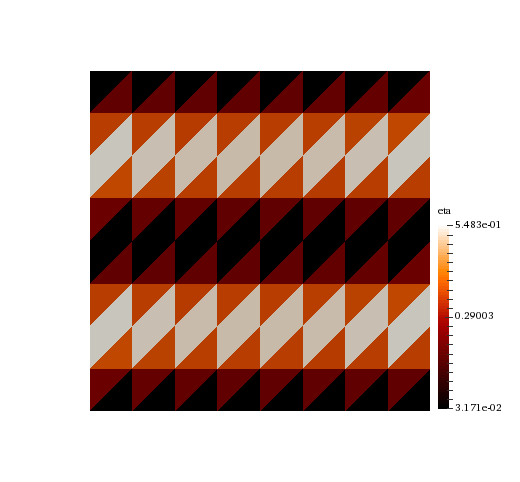
\includegraphics[width=\textwidth,height=\textheight,keepaspectratio,height=\textheight,keepaspectratio]{figures/poisson/P1/eta_8.png}
%    \caption{$N=8$}
%  \end{subfigure}
%  \begin{subfigure}[b]{0.24\textwidth}
%    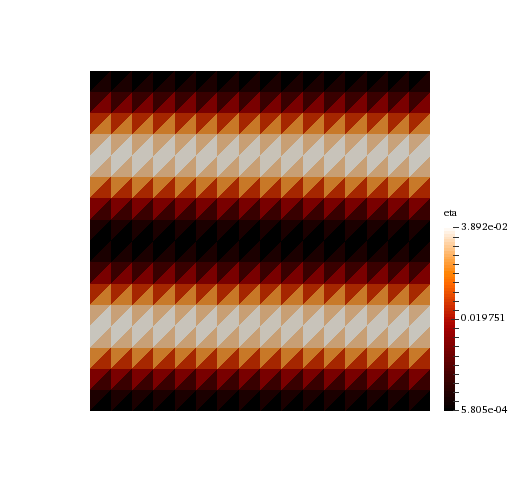
\includegraphics[width=\textwidth,height=\textheight,keepaspectratio,height=\textheight,keepaspectratio]{figures/poisson/P1/eta_16.png}
%    \caption{$N=16$}
%  \end{subfigure}
%  \begin{subfigure}[b]{0.24\textwidth}
%    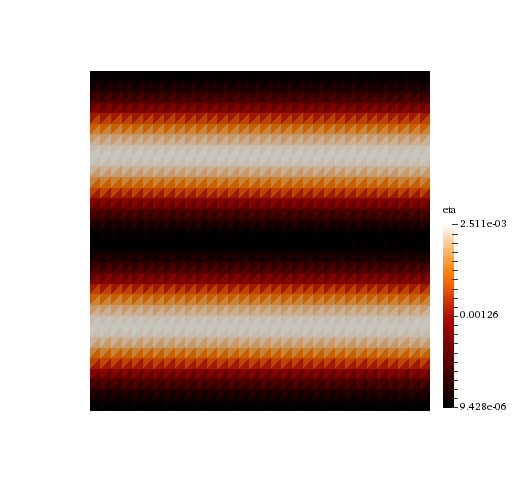
\includegraphics[width=\textwidth,height=\textheight,keepaspectratio,height=\textheight,keepaspectratio]{figures/poisson/P1/eta_32.png}
%    \caption{$N=32$}
%  \end{subfigure}
%  \begin{subfigure}[b]{0.24\textwidth}
%    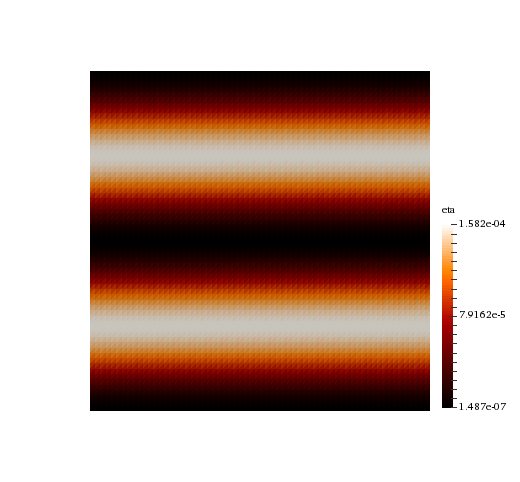
\includegraphics[width=\textwidth,height=\textheight,keepaspectratio,height=\textheight,keepaspectratio]{figures/poisson/P1/eta_64.png}
%    \caption{$N=64$}
%  \end{subfigure}
%  \caption{Error magnitude for $\eta$ for the Poisson model discretized with $P_1$ elements} \label{fig:poisson_eta_P1}
%\end{figure}
%\mbox{}\\
%\begin{figure}[h!]
%  \centering
%  \begin{subfigure}[b]{0.24\textwidth}
%    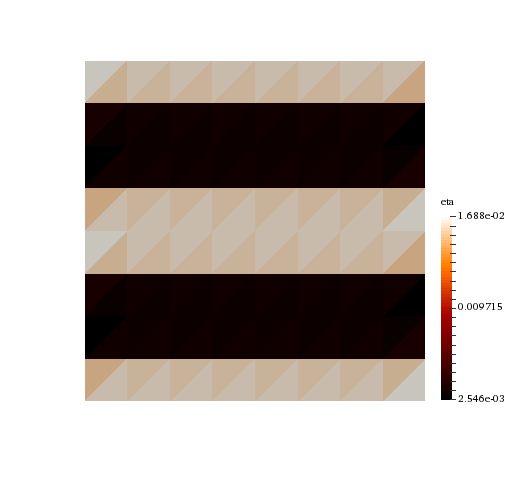
\includegraphics[width=\textwidth,height=\textheight,keepaspectratio,height=\textheight,keepaspectratio]{figures/poisson/P2/eta_8.png}
%    \caption{$N=8$}
%  \end{subfigure}
%  \begin{subfigure}[b]{0.24\textwidth}
%    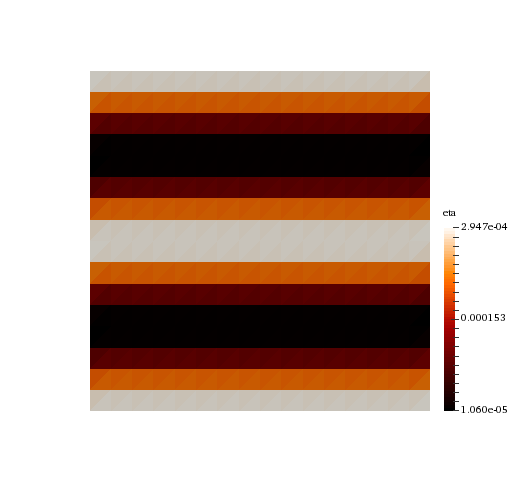
\includegraphics[width=\textwidth,height=\textheight,keepaspectratio,height=\textheight,keepaspectratio]{figures/poisson/P2/eta_16.png}
%    \caption{$N=16$}
%  \end{subfigure}
%  \begin{subfigure}[b]{0.24\textwidth}
%    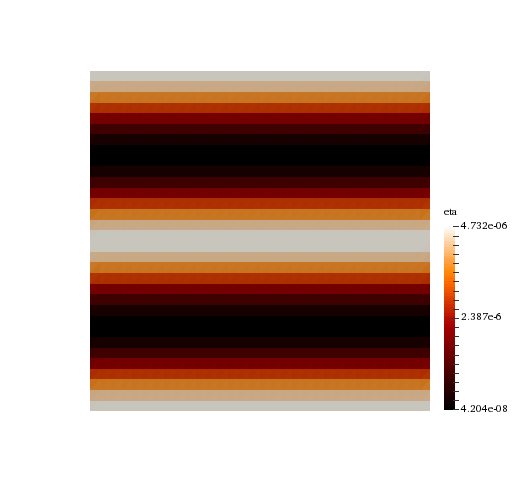
\includegraphics[width=\textwidth,height=\textheight,keepaspectratio,height=\textheight,keepaspectratio]{figures/poisson/P2/eta_32.png}
%    \caption{$N=32$}
%  \end{subfigure}
%  \begin{subfigure}[b]{0.24\textwidth}
%    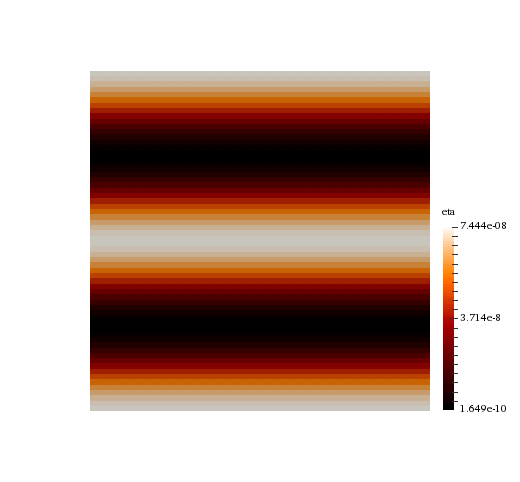
\includegraphics[width=\textwidth,height=\textheight,keepaspectratio,height=\textheight,keepaspectratio]{figures/poisson/P2/eta_64.png}
%    \caption{$N=64$}
%  \end{subfigure}
%  \caption{Error magnitude for $\eta$ for the Poisson model discretized with $P_2$ elements} \label{fig:poisson_eta_P2}
%\end{figure}
%\mbox{}\\
%\begin{figure}[h!]
%  \centering
%  \begin{subfigure}[b]{0.24\textwidth}
%    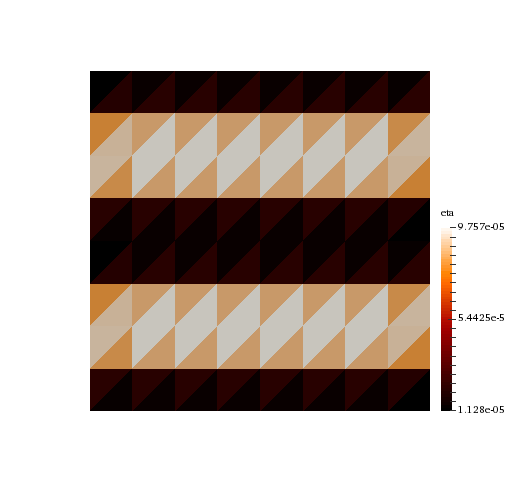
\includegraphics[width=\textwidth,height=\textheight,keepaspectratio,height=\textheight,keepaspectratio]{figures/poisson/P3/eta_8.png}
%    \caption{$N=8$}
%  \end{subfigure}
%  \begin{subfigure}[b]{0.24\textwidth}
%    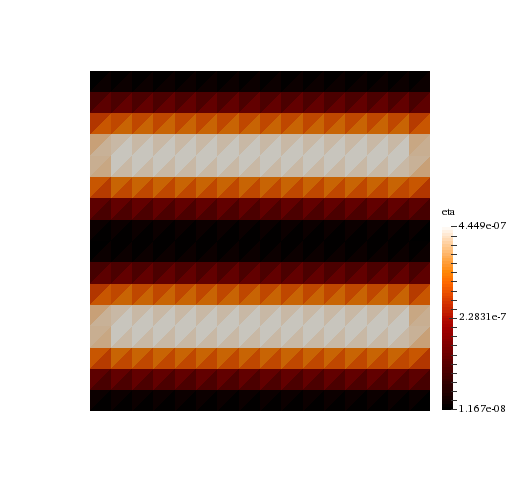
\includegraphics[width=\textwidth,height=\textheight,keepaspectratio,height=\textheight,keepaspectratio]{figures/poisson/P3/eta_16.png}
%    \caption{$N=16$}
%  \end{subfigure}
%  \begin{subfigure}[b]{0.24\textwidth}
%    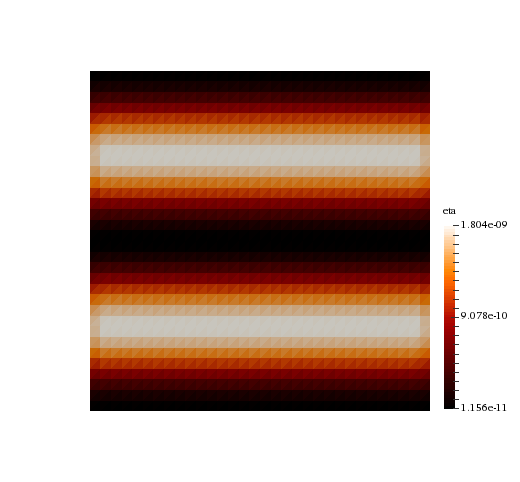
\includegraphics[width=\textwidth,height=\textheight,keepaspectratio,height=\textheight,keepaspectratio]{figures/poisson/P3/eta_32.png}
%    \caption{$N=32$}
%  \end{subfigure}
%  \begin{subfigure}[b]{0.24\textwidth}
%    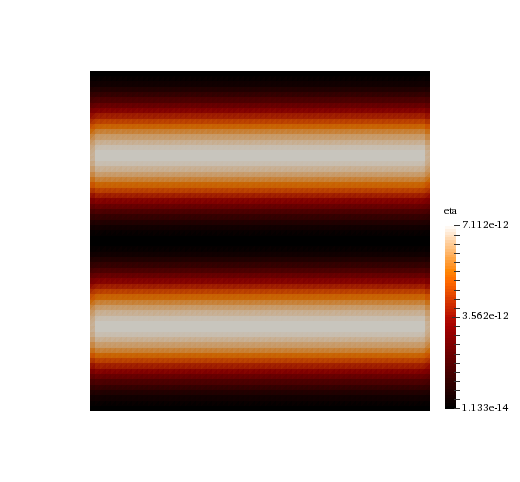
\includegraphics[width=\textwidth,height=\textheight,keepaspectratio,height=\textheight,keepaspectratio]{figures/poisson/P3/eta_64.png}
%    \caption{$N=64$}
%  \end{subfigure}
%  \caption{Error magnitude for $\eta$ for the Poisson model discretized with $P_3$ elements} \label{fig:poisson_eta_P3}
%\end{figure}
\mbox{}\\ \\
\section{Multiple network poroelasticity model (MPET)} \label{section:num_exp_mpet}
This section presents the numerical results from the computation of the a posteriori error estimator derived for the MPET model with a single network (Biot), two networks (Barenblatt-Biot) and a four-network poroelasticity model. The results are validated by computing convergence rates and comparing the results with the theoretical predictions. In addition, the error magnitude for each estimator will be displayed to demonstrate where potential mesh refinement should occur. Note that we will not perform any adaptive mesh refinement in this work. 
\\
\\
To numerically compute the MPET model, we use a manufactured solution and compute the error and convergence rates for the displacement and pressure discretized with Taylor-Hood elements. As we stated in chapter \ref{chap:discretization} we assume Dirichlet boundary conditions, where $u$ and $p$ are equal to some known function on the boundary. In this case, these known functions will be the manufactured solution. 

\subsection{Single network poroelasticity} \label{section:num_exp_mpet1}
In order to evaluate the a posteriori error estimates constructed for the single network poroelasticity model (i.e. the Biot model), we compute their convergence rates under space and time refinement. For the spatial refinement parameter we keep the time step $\tau$ fixed and refine the spatial discretization $h$, and for the temporal refinement, we keep $h$ fixed and refine $\tau$. The manufactured solution chosen for verification for the single network model (Biot) is:
\begin{align*}
u_e = & \, \left(\cos(\pi x)\sin(\pi y)\sin(\pi t), \, \sin(\pi x)\cos(\pi y)\sin(\pi t)\right) \\
p_e = & \, \sin(\pi x) \cos(\pi y)\sin(2\pi t)
\end{align*}
The source terms are found in the same way as described in section \ref{section:mms}. We evaluate the error estimators derived in section \ref{biot:res_err}, which stated that the spatial and temporal error $E$ from section \ref{biot:res_err} could be bounded in the following way,
\begin{equation} \label{biot:error_upbd}
E^n \leq \underbrace{\sup_{m \in [1,N]} (\eta^m_u}_{\eta_1})^\frac{1}{2}  +  \underbrace{(\sum_{m=1}^N \tau_m \eta^m_{p,0})^\frac{1}{2}}_{\eta_2} + \underbrace{\sum_{m=1}^N (\eta^m_u(\delta_t))^\frac{1}{2}}_{\eta_3} + \underbrace{(\sum_{m=1}^N \tau_m \| p_h^m - p_h^{m-1}\|^2_d)^\frac{1}{2}}_{\eta_4}
\end{equation}
\begin{remark}
Note that there are additional terms in $E^n$ other than $\|u - u_{h_{\tau}}\|_{H^1}$ and $\|p - p_{h_{\tau}}\|_{L^2}$. For simplicity, we will only compute these two terms as part of the error to be evaluated. In addition, we have disregarded the data oscillations terms, $\mathcal{E}_{\textnormal{dat}}$ and focused solely on the space and time estimators.
\end{remark}
\mbox{}\\
The a posteriori error estimators indicate how the error behaves in space and time. The space estimator $\eta_1$ is associated with the residual of the displacement $u$, and $\eta_2$ is associated with the residual of the pressure $p$. $\eta_3$ predicts how time may affect the residual of the displacement under space refinement. In other words, $\eta_3$ will indicate how the displacement-residual may change from one time step to the other when we refine in space. Thus, if $\eta_1$ is small compared to $\eta_3$, we should refine in time. Conversely, if $\eta_3$ is small compared to $\eta_1$, we should refine in space. The magnitude of these two estimators indicates \textit{how} to refine. $\eta_4$ is a time estimator associated with the pressure. 
\\
\\
Table \ref{tab:biot_default_space_error} displays the error and convergence rate for the displacement and the pressure under space refinement. We observe that setting all parameters to 1 yields optimal convergence rates for both the displacement and the pressure. The a posteriori error estimators demonstrate optimal order of convergence for $\eta_1$ and $\eta_2$ under space refinement, see table \ref{tab:biot_default_space_est}. Table \ref{tab:biot_default_time_error} presents the error and convergence rate for the displacement and the pressure under space refinement, which yields optimal rates. We also observe optimal rates for the time estimator $\eta_4$ under time refinement, see table \ref{tab:biot_default_time_error}. The error magnitude for the space estimators is illustrated in figures \ref{fig:biot_eta1}, \ref{fig:biot_eta2} and \ref{fig:biot_eta3} for the single network model under space refinement. We observe that the resolution increases as the mesh is refined, which gives an indication where we should concentrate our refinement. The magnitude of $\eta_3$ is much smaller than $\eta_1$, and thus suggests further refinement in space. The error estimators for the displacement and the pressure are different, which gives valuable information regarding how the error for each component behaves under space refinement. That way we can make an informed decision on how to refine, e.g. if we wish to make the solution for $p$ more accurate in space we concentrate the adaptive refinement in the areas indicated by $\eta_2$.
\\
\\
According to the analysis presented in \cite{meunier}, the correct order of convergence for $\eta_3$ should be 2 under space refinement. This is because it is based on the residual of the first equation, which is associated with the displacement. We have already established that we expect second-order convergence for the displacement in the $H^1$-norm when approximated by piecewise quadratics. However, since $\eta_3$ is a time incremental version of $\eta_1$ which is approximated with Backward Euler in time, it may also be reasonable to expect this estimator to converge as a time estimator. %Observing an order lower than expected may be due to errors occurring when we numerically compute the divergence of the stress tensor in FEniCS. 
In addition, we observe that the time estimator $\eta_4$ does not decrease as the mesh is refined, but stays constant. This can be explained by the fact that since it is a time estimator, it may exhibit space-independence when the time step is small compared to the spatial refinement parameter. Figure \ref{fig:biot_eta4} displays the error magnitude for the time estimator $\eta_4$ under time refinement. The lighter areas indicate higher error concentration, which indicates a potential for adaptive refinement. %In order to investigate why we observe incorrect rates, space/time-refinement are presented in tables \ref{tab:biot_default_time_space_eta1}, \ref{tab:biot_default_time_space_eta2}, \ref{tab:biot_default_time_space_eta3}, \ref{tab:biot_default_time_space_eta4} for $\eta_1$, $\eta_2$, $\eta_3$ and $\eta_4$, respectively. \todo{explain space/time tables!}
%%%%%%%%%%%%%%%%%%%%%%%%%%%%%%%%%%%%%%%%%%%%%%%%%%%%%%
\\
\\
\begin{center} 
\centering
\begin{tabular}{c|c|c|c|c}
$h^{-1}$ & $\|u - u_{h_{\tau}}\|_{H^1}$ & Rate & $\|p - p_{h_{\tau}}\|_{L^2}$ & Rate\\\hline
4  & 1.947e-2 & -     & 1.788e-3 & - \\
8  & 4.693e-3 & 2.053 & 6.245e-4 & 1.518 \\
16 & 1.141e-3 & 2.041 & 1.755e-4 & 1.832 \\
32 & 2.835e-4 & 2.008 & 4.313e-5 & 2.024 \\
64 & 7.192e-5 & 1.979 & 1.026e-5 & 2.072 \\\hline
Opt. & & 2 & & 2 
\end{tabular}
\captionof{table}{Error norms and convergence rates for Biot model under space refinement, $T=0.1$, $\tau = 5.0$e-5, $\mu=0.5$, all other parameters set to $1$} \label{tab:biot_default_space_error}
\end{center}
\mbox{}\\ \\
\begin{center} 
\centering
\begin{tabular}{c|c|c|c|c|c|c|c}
$h^{-1}$ & $\eta_1$ & Rate &  $\eta_2$ & Rate & $\eta_3$ & Rate & $\eta_4$\\\hline
4  & 9.015e-1 & -     & 3.621e-1 & -     & 1.509e-3 & -     & 2.027e-4 \\
8  & 2.343e-1 & 1.944 & 2.002e-1 & 0.855 & 7.763e-4 & 0.959 & 2.060e-4 \\
16 & 5.916e-2 & 1.986 &1.034e-1  & 0.954 & 3.913e-4 & 0.988 & 2.066e-4 \\
32 & 1.483e-2 & 1.996 & 5.232e-2 & 0.982 & 1.961e-4 & 0.997 & 2.068e-4 \\
64 & 3.711e-3 & 1.999 & 2.630e-2 & 0.992 & 9.810e-5 & 0.999 & 2.068e-4 \\\hline
Opt. & & 2 & & 1 & & 2\footnote[1]{According to \cite{meunier}, the correct order of convergence for $\eta_3$ should be 2.} & 
\end{tabular}
\captionof{table}{Convergence rate for a posteriori error estimates for the Biot model under space refinement, $T=0.1$, $\tau = 5.0$e-5, $\mu=0.5$, all other parameters set to $1$} \label{tab:biot_default_space_est}

\clearpage
\begin{center}
\centering
\begin{tabular}{c|c|c|c|c}
$\tau$ & $\|u-u_{h_{\tau}}\|_{H^1}$ & Rate & $\|p-p_{h_{\tau}}\|_{L^2}$ & Rate \\\hline
0.02    & 1.392e-3 & -     & 4.184e-3 & -     \\
0.01    & 5.838e-4 & 1.253 & 1.768e-3 & 1.243 \\
0.005   & 2.644e-4 & 1.143 & 8.026e-4 & 1.139 \\
0.0025  & 1.203e-4 & 1.136 & 3.657e-4 & 1.134 \\
0.00125 & 6.079e-5 & 0.985 & 1.828e-4 & 1.000 \\ \hline
Opt. & & 1 & & 1 
\end{tabular}
\captionof{table}{A priori error estimates, a posteriori error estimates and convergence rates for the Biot model under time refinement, $T=1$, $h=1/128$, $\mu=0.5$, all other parameters set to $1$} \label{tab:biot_default_time_error}
\end{center}
\end{center}
\mbox{}\\ \\
\begin{center} 
\centering
\begin{tabular}{c|c|c|c|c|c}
$\tau$ & $\eta_1$ & $\eta_2$ & $\eta_3$ & $\eta_4$ & Rate\\\hline
0.02    & 2.947e-3 & 8.375e-2 & 1.961e-2 & 1.923e-1 & -    \\
0.01    & 2.947e-3 & 8.411e-2 & 9.809e-3 & 9.742e-2 & 0.981\\
0.005   & 2.948e-3 & 8.431e-2 & 4.905e-3 & 4.903e-2 & 0.991\\
0.0025  & 2.948e-3 & 8.441e-2 & 2.453e-3 & 2.466e-2 & 0.992\\
0.00125 & 2.948e-3 & 8.446e-2 & 1.226e-3 & 1.233e-2 & 0.999\\\hline
Opt. & & & & & 1
\end{tabular}
\captionof{table}{Convergence rate for a posteriori error estimates for the Biot model under time refinement, $T=1$, $h=1/128$, $\mu=0.5$, all other parameters set to $1$} \label{tab:biot_default_time_est}
\end{center}
\mbox{}\\ \\
\begin{figure}[h!]
  \centering
  \begin{subfigure}[b]{0.24\textwidth}
    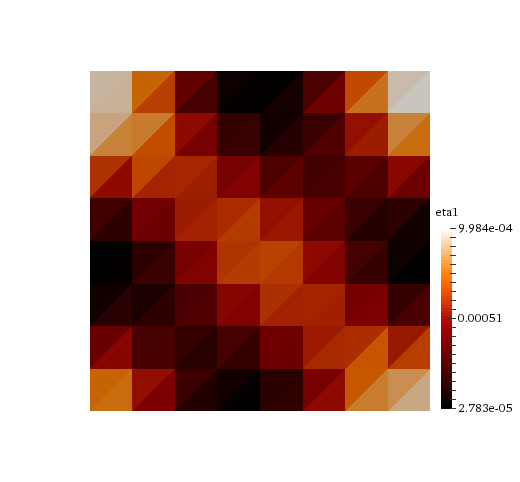
\includegraphics[width=\textwidth,height=\textheight,keepaspectratio,height=\textheight,keepaspectratio]{figures/1_mpet/space/eta1_8.png}
    \caption{$N=8$}
  \end{subfigure}
  \begin{subfigure}[b]{0.24\textwidth}
    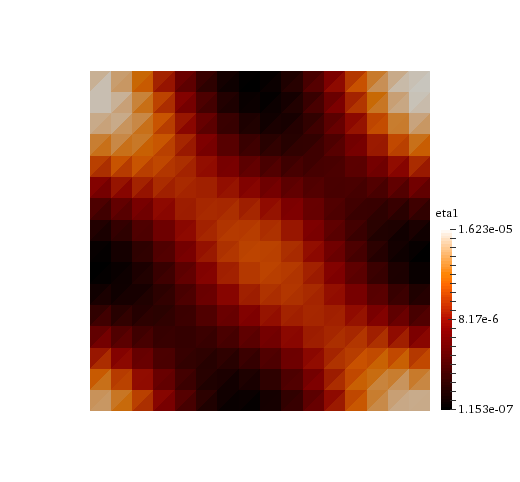
\includegraphics[width=\textwidth,height=\textheight,keepaspectratio,height=\textheight,keepaspectratio]{figures/1_mpet/space/eta1_16.png}
    \caption{$N=16$}
  \end{subfigure}
  \begin{subfigure}[b]{0.24\textwidth}
    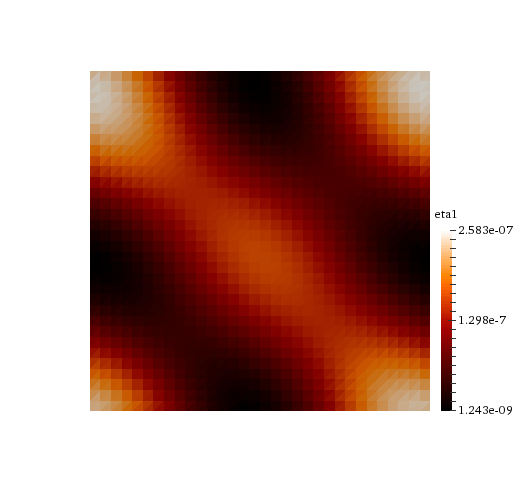
\includegraphics[width=\textwidth,height=\textheight,keepaspectratio,height=\textheight,keepaspectratio]{figures/1_mpet/space/eta1_32.png}
    \caption{$N=32$}
  \end{subfigure}
  \begin{subfigure}[b]{0.24\textwidth}
    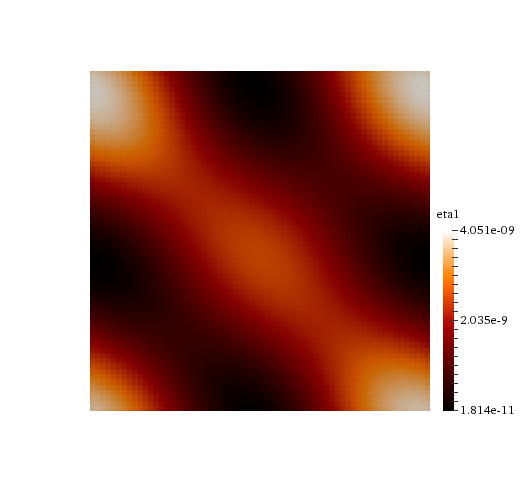
\includegraphics[width=\textwidth,height=\textheight,keepaspectratio,height=\textheight,keepaspectratio]{figures/1_mpet/space/eta1_64.png}
    \caption{$N=64$}
  \end{subfigure}
  \caption{Error magnitude for $\eta_1$ under space refinement at $t=T$ for single network MPET model} \label{fig:biot_eta1}
\end{figure}

\clearpage

\begin{figure}[h!]
  \centering
  \begin{subfigure}[b]{0.24\textwidth}
    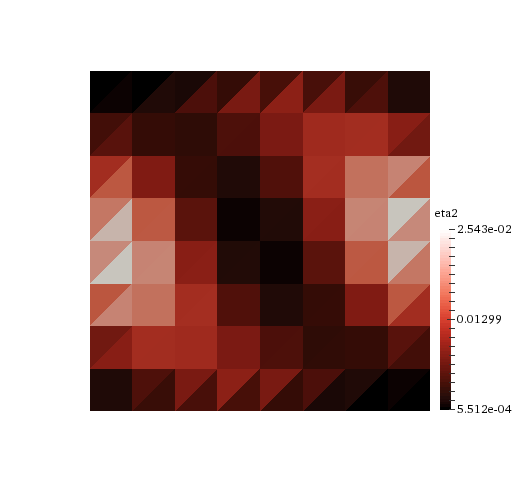
\includegraphics[width=\textwidth,height=\textheight,keepaspectratio,height=\textheight,keepaspectratio]{figures/1_mpet/space/eta2_8.png}
    \caption{$N=8$}
  \end{subfigure}
  \begin{subfigure}[b]{0.24\textwidth}
    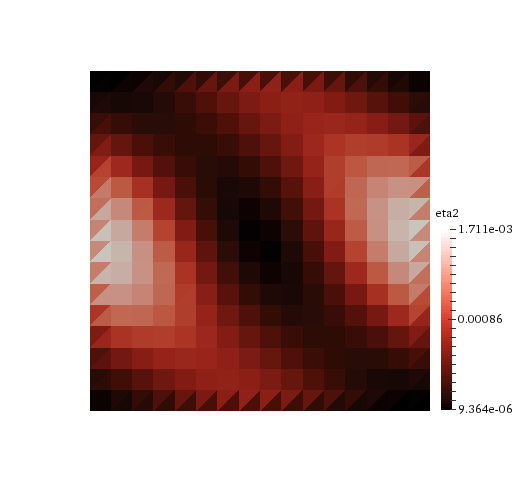
\includegraphics[width=\textwidth,height=\textheight,keepaspectratio,height=\textheight,keepaspectratio]{figures/1_mpet/space/eta2_16.png}
    \caption{$N=16$}
  \end{subfigure}
  \begin{subfigure}[b]{0.24\textwidth}
    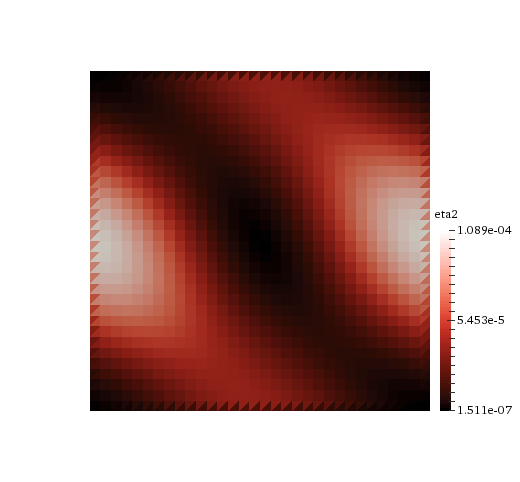
\includegraphics[width=\textwidth,height=\textheight,keepaspectratio,height=\textheight,keepaspectratio]{figures/1_mpet/space/eta2_32.png}
    \caption{$N=32$}
  \end{subfigure}
  \begin{subfigure}[b]{0.24\textwidth}
    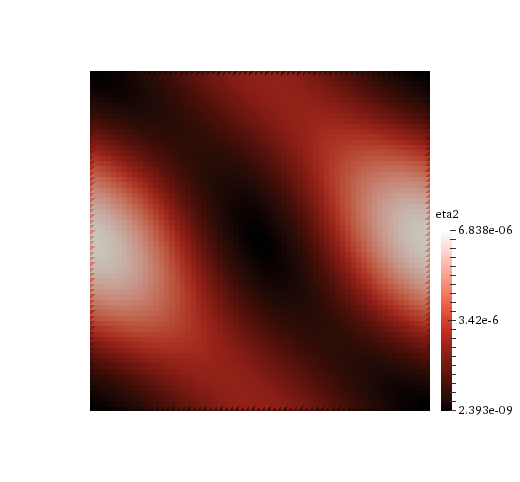
\includegraphics[width=\textwidth,height=\textheight,keepaspectratio,height=\textheight,keepaspectratio]{figures/1_mpet/space/eta2_64.png}
    \caption{$N=64$}
  \end{subfigure}
  \caption{Error magnitude for $\eta_2$ under space refinement at $t=T$ for single network MPET model} \label{fig:biot_eta2}
\end{figure}
\mbox{}\\ \\
\begin{figure}[h!]
  \centering
  \begin{subfigure}[b]{0.24\textwidth}
    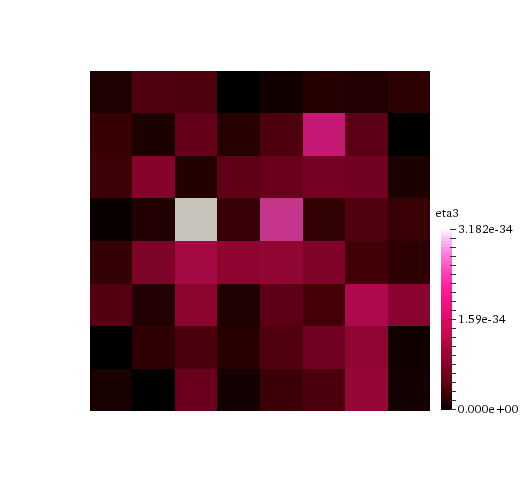
\includegraphics[width=\textwidth,height=\textheight,keepaspectratio,height=\textheight,keepaspectratio]{figures/1_mpet/space/eta3_8.png}
    \caption{$N=8$}
  \end{subfigure}
  \begin{subfigure}[b]{0.24\textwidth}
    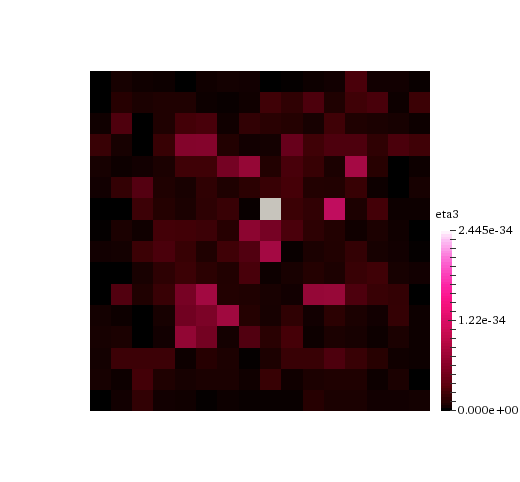
\includegraphics[width=\textwidth,height=\textheight,keepaspectratio,height=\textheight,keepaspectratio]{figures/1_mpet/space/eta3_16.png}
    \caption{$N=16$}
  \end{subfigure}
  \begin{subfigure}[b]{0.24\textwidth}
    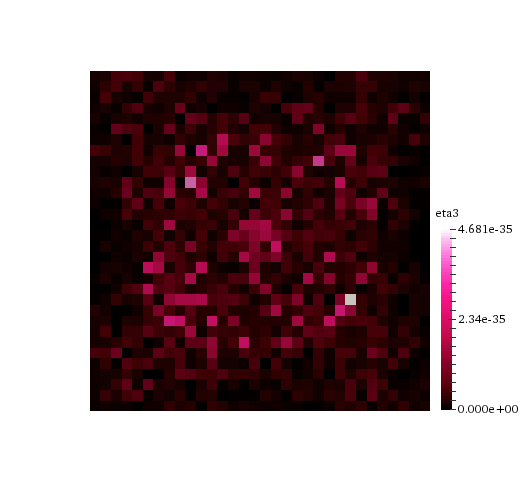
\includegraphics[width=\textwidth,height=\textheight,keepaspectratio,height=\textheight,keepaspectratio]{figures/1_mpet/space/eta3_32.png}
    \caption{$N=32$}
  \end{subfigure}
  \begin{subfigure}[b]{0.24\textwidth}
    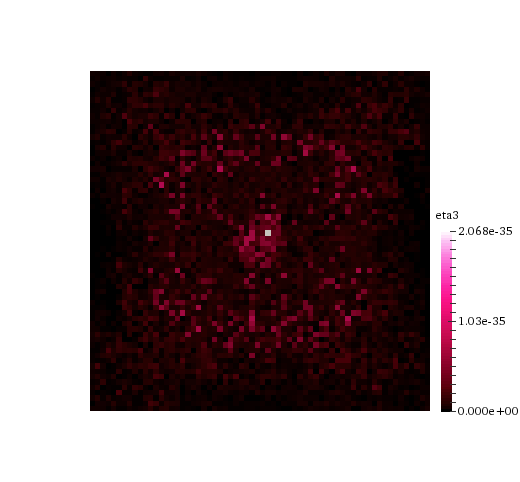
\includegraphics[width=\textwidth,height=\textheight,keepaspectratio,height=\textheight,keepaspectratio]{figures/1_mpet/space/eta3_64.png}
    \caption{$N=64$}
  \end{subfigure}
  \caption{Error magnitude for $\eta_3$ under space refinement at $t=T$ for single network MPET model} \label{fig:biot_eta3}
\end{figure}
\mbox{}\\ \\
\begin{figure}[h!]
  \centering
  \begin{subfigure}[b]{0.24\textwidth}
    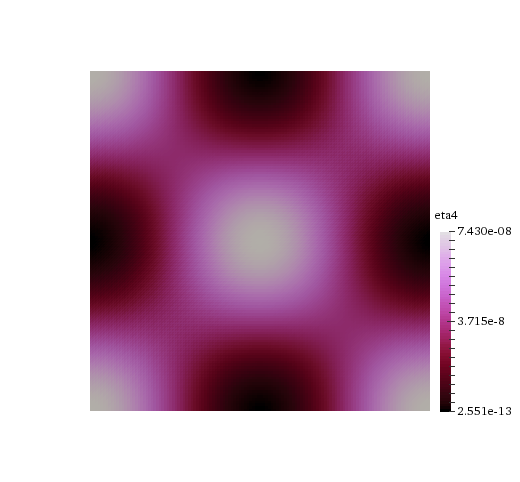
\includegraphics[width=\textwidth,height=\textheight,keepaspectratio,height=\textheight,keepaspectratio]{figures/1_mpet/time/eta4_dt1.png}
    \caption{$\tau=0.01$}
  \end{subfigure}
  \begin{subfigure}[b]{0.24\textwidth}
    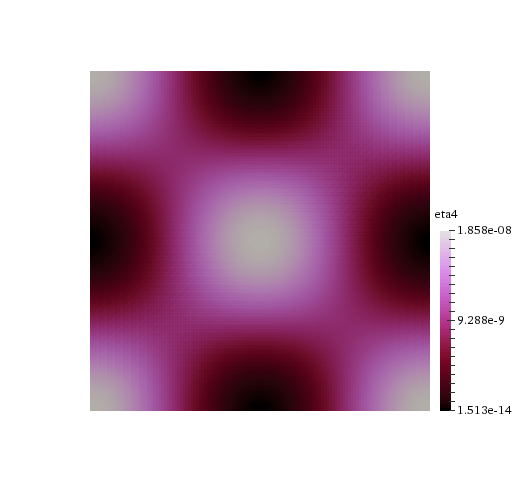
\includegraphics[width=\textwidth,height=\textheight,keepaspectratio,height=\textheight,keepaspectratio]{figures/1_mpet/time/eta4_dt2.png}
    \caption{$\tau=0.005$}
  \end{subfigure}
  \begin{subfigure}[b]{0.24\textwidth}
    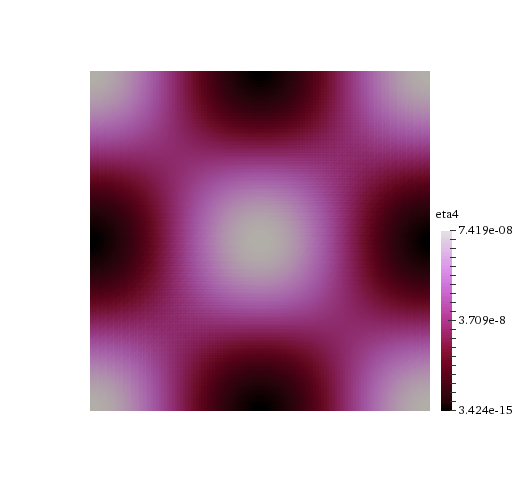
\includegraphics[width=\textwidth,height=\textheight,keepaspectratio,height=\textheight,keepaspectratio]{figures/1_mpet/time/eta4_dt3.png}
    \caption{$\tau=0.0025$}
  \end{subfigure}
  \begin{subfigure}[b]{0.24\textwidth}
    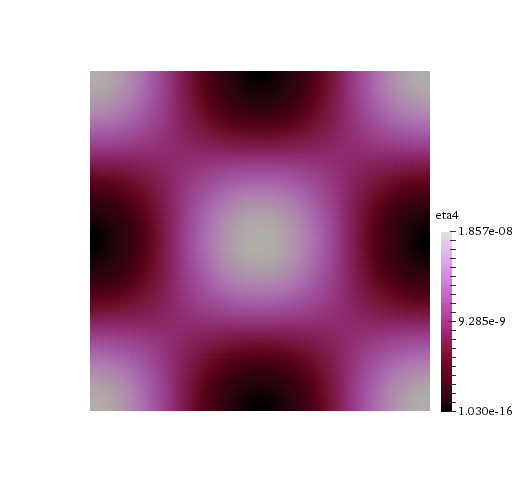
\includegraphics[width=\textwidth,height=\textheight,keepaspectratio,height=\textheight,keepaspectratio]{figures/1_mpet/time/eta4_dt4.png}
    \caption{$\tau=0.00125$}
  \end{subfigure}
  \caption{Error magnitude for $\eta_4$ under time refinement at $t=T$ for single network MPET model} \label{fig:biot_eta4}
\end{figure}
\clearpage
%\begin{center} 
%\centering
%\begin{tabular}{c|c|c|c|c}
%$\tau$ / $h^{-1}$ & 4        & 8        & 16      & 32    \\\hline
%$1/4^2$   & 2.865e+0 & 7.440e-1 & 1.878e-1 & 4.707e-2 \\   
%$1/8^2$   & 2.867e+0 & 7.446e-1 & 1.879e-1 & 4.710e-2 \\
%$1/16^2$  & 2.868e+0 & 7.448e-1 & 1.879e-1 & 4.711e-2 \\
%$1/32^2$  & 2.868e+0 & 7.448e-1 & 1.879e-1 & 4.711e-2 \\
%\end{tabular}
%\captionof{table}{Error estimates for $\eta_1$ under space/time refinement, $T=1$, $\mu=0.5$, all other parameters set to $1$} \label{tab:biot_default_time_space_eta1}
%\end{center}
%\mbox{}\\
%\begin{center} 
%\centering
%\begin{tabular}{c|c|c|c|c}
%$\tau$ / $h^{-1}$ & 4        & 8        & 16      & 32    \\\hline
%$1/4^2$   & 2.216e+0 & 1.243e+0 & 6.465e-1 & 3.279e-1 \\   
%$1/8^2$   & 2.224e+0 & 1.257e+0 & 6.553e-1 & 3.327e-1 \\
%$1/16^2$  & 2.230e+0 & 1.262e+0 & 6.586e-1 & 3.344e-1 \\
%$1/32^2$  & 2.231e+0 & 1.263e+0 & 6.594e-1 & 3.349e-1 \\
%\end{tabular}
%\captionof{table}{Error estimates for $\eta_2$ under space/time refinement, $T=1$, $\mu=0.5$, all other parameters set to $1$} \label{tab:biot_default_time_space_eta2}
%\end{center}
%\mbox{}\\
%\begin{center} 
%\centering
%\begin{tabular}{c|c|c|c|c}
%$\tau$ / $h^{-1}$ & 4 & 8 & 16 & 32    \\\hline
%$1/4^2$  & 1.873e+0 & 9.637e-1 & 4.858e-1 & 2.434e-1 \\   
%$1/8^2$  & 4.714e-1 & 2.425e-1 & 1.222e-1 & 6.125e-2 \\
%$1/16^2$ & 1.179e-1 & 6.064e-2 & 3.057e-2 & 1.532e-2 \\
%$1/32^2$ & 2.948e-2 & 1.516e-2 & 7.643e-3 & 3.830e-3 \\
%\end{tabular}
%\captionof{table}{Error estimates for $\eta_3$ under space/time refinement, $T=1$, $\mu=0.5$, all other parameters set to $1$} \label{tab:biot_default_time_space_eta3}
%\end{center}
%\mbox{}\\
%\begin{center}
%\centering
%\begin{tabular}{c|c|c|c|c}
%$\tau$ / $h^{-1}$ & 4        & 8        & 16      & 32    \\\hline
%$1/4^2$   & 5.881e-1 & 5.999e-1 & 6.029e-1 & 6.037e-1 \\   
%$1/8^2$   & 1.489e-1 & 1.523e-1 & 1.532e-1 & 1.534e-1 \\
%$1/16^2$  & 3.730e-2 & 3.820e-2 & 3.843e-2 & 3.849e-2 \\
%$1/32^2$  & 9.331e-3 & 9.556e-3 & 9.616e-3 & 9.631e-3 \\
%\end{tabular}
%\captionof{table}{Error estimates for $\eta_4$ under space/time refinement, $T=1$, $\mu=0.5$, all other parameters set to $1$}  \label{tab:biot_default_time_space_eta4}
%\end{center}

\subsection{Two-network poroelasticity} \label{test_bb}
For the two-network poroelasticity model (Barenblatt-Biot) we use the following manufactured solution,
\begin{align*}
u_e = & \, \left(\cos(\pi x)\sin(\pi y)\sin(\pi t), \, \sin( \pi x)\cos(\pi y)\sin(\pi t)\right) \\
p_{1_e} = & \,\sin(\pi x) \cos(\pi y)\sin(2\pi t)  \\
p_{2_e} = & \,\cos(\pi x) \sin(\pi y)\sin(2\pi t)
\end{align*}
This section presents the numerical results obtained from computing the a posteriori error estimates constructed for the two-network poroelasticity model (i.e. the Barenblatt-Biot model) in section  \ref{section:error_bb}. The results include both a spatial and temporal refinement, with the same discretization parameters as for the single network model. The estimators have been implemented using the test problem described in section \ref{test_bb} using Taylor-Hood elements.
\\
\\
We use the error estimators derived in section \ref{bb:case1_res_err}, which stated that the spatial and temporal error $E$ from \eqref{bb:error} could be bounded in the following way,
\begin{align} 
E^n \leq & \underbrace{\sup_{m \in [1,N]} (\eta^m_u)^\frac{1}{2}}_{\eta_1} + \underbrace{\left(\sum_{m=1}^N \tau_m \eta^m_{p_1,0} + \eta^m_{p_2,0}\right)^\frac{1}{2}}_{\eta_2} + \underbrace{\sum_{m=1}^N (\eta^m_u(\delta_t))^\frac{1}{2}}_{\eta_3} \\
& + \underbrace{\left(\sum_{m=1}^N \tau_m (\|p^m_{1h} - p^{m-1}_{1h}\|_d^2 + \|p^m_{2h} - p^{m-1}_{2h}\|_d^2) )\right)^\frac{1}{2}}_{\eta_4}
\end{align}
\begin{remark}
Note that there are additional terms in $E^n$ other than $\|u - u_{h_{\tau}}\|_{H^1}$, $\|p_1 - p_{1h_{\tau}}\|_{L^2}$ and $\|p_2 - p_{2h_{\tau}}\|_{L^2}$. For simplicity, we will only compute these two terms as part of the error to be evaluated. In addition, we have disregarded the data oscillations terms, $\mathcal{E}_{\textnormal{dat}}$ and focused solely on the space and time estimators for the numerical experiments.
\end{remark}
\mbox{}\\
The a posteriori error estimators indicate how the error behaves in space and time. The space estimator $\eta_1$ is associated with the residual of the displacement $u$, and $\eta_2$ is associated with the residual of the pressures $p_1$ and $p_2$. $\eta_3$ predicts how time may affect the residual of the displacement under space refinement. The magnitude of these two estimators gives an indication of \textit{how} to refine. $\eta_4$ is a time estimator associated with the pressure. 
\\
\\
The first experiment is implemented assuming non-interacting fluid networks, with $\mu = 0.5$, $\xi_1 = \xi_2 = 0$ and all other parameters to $1$. The same experiment is then executed with interacting fluid networks. Additionally, an experiment with physiologically inspired parameters is presented.  
\\
\subsubsection{Two-network poroelasticity: non-interacting fluid networks}
Table \ref{tab:bb_no_transfer_space_error} present the convergence rates for the a priori error estimate for the displacement and the pressures under space refinement with non-interacting fluid networks. The displacement and the pressure converge optimally as the mesh is refined. We observe that the a posteriori error estimators yields the same rates as for the Biot model, where we see one order lower for $\eta_3$ than what is expected according to \cite{meunier}, see table \ref{tab:bb_no_transfer_space_est}. The quantity $\eta_4$, which is associated with the time error remains constant under space refinement. Figures \ref{fig:bb_no_transfer_eta1}, \ref{fig:bb_no_transfer_eta2} and \ref{fig:bb_no_transfer_eta3} present the error magnitude for the space estimators for the two-network model under space refinement. Similarly, as with the single network model, the magnitude for $\eta_3$ is much smaller than $\eta_1$ indicating further space refinement, and not time refinement. Recall that $\eta_3$ is a space estimator predicting the effect of time on the displacement under space refinement. Thus, when this quantity is much smaller than the space estimator for the displacement suggests adaptive refinement in space. The quantity $\eta_1$ predicts how the spatial error for $u$ will behave, while $\eta_2$ predicts the behavior of the spatial error for the pressures $p_1$ and $p_2$.
\\
\\
Table \ref{tab:bb_no_transfer_time_error} displays the convergence rate for the a priori error estimate for the displacement and the pressures under time refinement with non-interacting fluid networks. The displacement and the pressure exhibit optimal convergence as the time step is refined. Running simulations with smaller time steps ensure convergence of order 1. The time estimator $\eta_4$ converges optimally, see table \ref{tab:bb_no_transfer_time_est}. Figure \ref{fig:bb_no_transfer_eta4} displays the time estimator $\eta_4$ under time refinement. We observe that the overall accuracy of the error increases under time refinement. The lighter areas indicate a higher error, which suggests a potential adaptive refinement to be concentrated here. 
\\
\\
\begin{center} 
\centering
\begin{tabular}{c|c|c|c|c|c|c}
$h^{-1}$ & $\|u - u_{h_{\tau}}\|_{H^1}$ & Rate & $\|p_1 - p_{1h_{\tau}}\|_{L^2}$ & Rate & $\|p_2 - p_{2h_{\tau}}\|_{L^2}$ & Rate\\\hline
4  & 3.458e-2 & -     & 1.999e-3 & -     & 1.999e-3 & - \\
8  & 8.318e-3 & 2.055 & 9.255e-4 & 1.111 & 9.255e-4 & 1.111 \\
16 & 2.038e-3 & 2.029 & 2.641e-4 & 1.809 & 2.641e-4 & 1.809 \\
32 & 5.081e-4 & 2.004 & 6.615e-5 & 1.997 & 6.615e-5 & 1.997 \\
64 & 1.286e-4 & 1.982 & 1.543e-5 & 2.100 & 1.543e-5 & 2.100 \\\hline
Opt. & & 2 & & 2 & & 2
\end{tabular}
\captionof{table}{Error norms and convergence rates for Barenblatt-Biot model with non-interacting fluid networks under space refinement, $T=0.1$, $\tau = 5.0$e-5, $\mu=0.5$, $\xi_1 = \xi_2 = 0$, all other parameters set to $1$} \label{tab:bb_no_transfer_space_error}
\end{center}

\clearpage

\begin{center} 
\centering
\begin{tabular}{c|c|c|c|c|c|c|c}
$h^{-1}$ & $\eta_1$ & Rate &  $\eta_2$ & Rate & $\eta_3$ & Rate & $\eta_4$\\\hline
4  & 9.626e-1 & -     & 5.172e-1 & -     & 1.530e-3 & -     & 2.875e-4 \\
8  & 2.454e-1 & 1.972 & 2.839e-1 & 0.865 & 7.860e-4 & 0.961 & 2.915e-4 \\
16 & 6.167e-2 & 1.992 & 1.462e-1 & 0.958 & 3.961e-4 & 0.988 & 2.922e-4 \\
32 & 1.544e-2 & 1.998 & 7.396e-2 & 0.983 & 1.985e-4 & 0.997 & 2.924e-4 \\
64 & 3.863e-3 & 1.999 & 3.717e-2 & 0.993 & 9.930e-5 & 0.999 & 2.924e-4 \\\hline
Opt. & & 2 & & 1  & & 2 & 
\end{tabular}
\captionof{table}{Convergence rate for a posteriori error estimates for the Barenblatt-Biot model with non-interacting fluid networks under space refinement, $T=0.1$, $\tau = 5.0$e-5, $\mu=0.5$, $\xi_1 = \xi_2 = 0$, all other parameters set to $1$} \label{tab:bb_no_transfer_space_est}
\end{center}
\mbox{}\\ \\ \\
\begin{center} 
\centering
\small
\begin{tabular}{c|c|c|c|c|c|c}
$\tau$ & $\|u-u_{h_{\tau}}\|_{H^1}$ & Rate & $\|p_1-p_{1h_{\tau}}\|_{L^2}$ & Rate & $\|p_2-p_{2h_{\tau}}\|_{L^2}$ & Rate \\\hline
0.02   	& 2.912e-3 & -     & 4.508e-3 & -     & 4.508e-3 &  -    \\
0.01   	& 1.258e-3 & 1.210 & 1.938e-3 & 1.218 & 1.938e-3 & 1.218 \\
0.005  	& 5.807e-4 & 1.116 & 8.900e-4 & 1.123 & 8.900e-4 & 1.123 \\
0.0025  & 2.798e-4 & 1.053 & 4.261e-4 & 1.062 & 4.261e-4 & 1.062 \\
0.00125 & 1.392e-4 & 1.007 & 2.095e-4 & 1.025 & 2.095e-4 & 1.025 \\ \hline
Opt. & & 1 & & 1  & & 1
\end{tabular}
\normalsize
\captionof{table}{Error estimates and convergence rates for the Barenblatt-Biot model with non-interacting fluid networks under time refinement, $T=1$, $h=1/128$, $\mu=0.5$, $\xi_1 = \xi_2 = 0$, all other parameters set to $1$} \label{tab:bb_no_transfer_time_error}
\end{center}
\mbox{}\\ \\ \\
\begin{center} 
\centering
\begin{tabular}{c|c|c|c|c|c}
$\tau$ & $\eta_1$ & $\eta_2$ & $\eta_3$ & $\eta_4$ & Rate\\\hline
0.02    & 2.948e-3 & 1.185e-1 & 1.985e-2 & 2.719e-1 & -    \\
0.01    & 2.947e-3 & 1.190e-1 & 9.930e-3 & 1.378e-1 & 0.981\\
0.005   & 2.947e-3 & 1.192e-1 & 4.965e-3 & 6.934e-2 & 0.991\\
0.0025  & 2.948e-3 & 1.194e-1 & 2.483e-3 & 3.478e-2 & 0.992\\
0.00125 & 2.948e-3 & 1.194e-1 & 1.241e-3 & 1.742e-2 & 0.998\\\hline
Opt. & & & & & 1
\end{tabular}
\captionof{table}{A posteriori error and convergence rates for the Barenblatt-Biot model with non-interacting fluid networks under time refinement, $T=1$, $h=1/128$, $\mu=0.5$, $\xi_1 = \xi_2 = 0$, all other parameters set to $1$} \label{tab:bb_no_transfer_time_est}
\end{center}

\begin{figure}[h!]
  \centering
  \begin{subfigure}[b]{0.24\textwidth}
    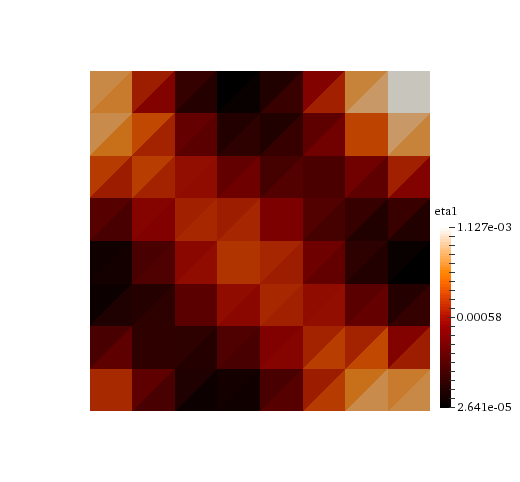
\includegraphics[width=\textwidth,height=\textheight,keepaspectratio,height=\textheight,keepaspectratio]{figures/2_mpet/no_transfer/space/eta1_8.png}
    \caption{$N=8$}
  \end{subfigure}
  \begin{subfigure}[b]{0.24\textwidth}
    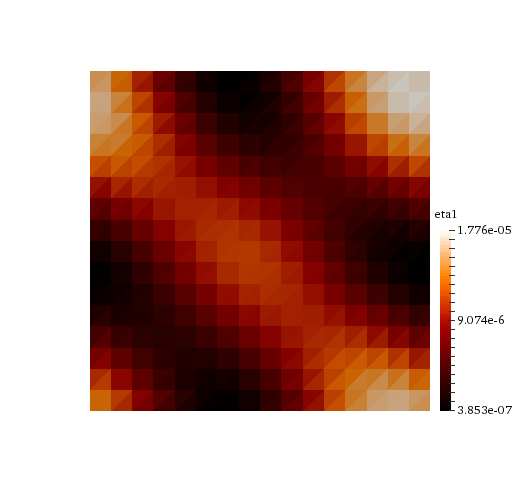
\includegraphics[width=\textwidth,height=\textheight,keepaspectratio,height=\textheight,keepaspectratio]{figures/2_mpet/no_transfer/space/eta1_16.png}
    \caption{$N=16$}
  \end{subfigure}
  \begin{subfigure}[b]{0.24\textwidth}
    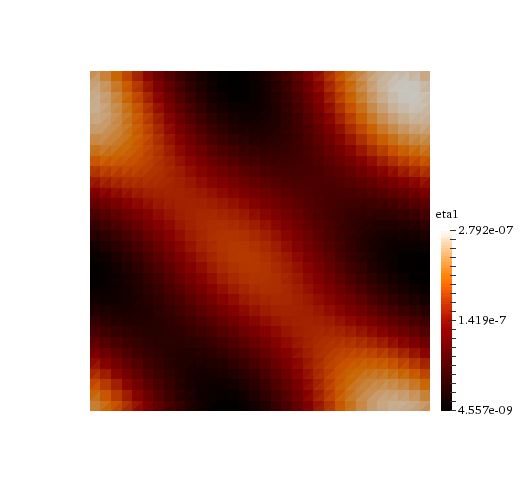
\includegraphics[width=\textwidth,height=\textheight,keepaspectratio,height=\textheight,keepaspectratio]{figures/2_mpet/no_transfer/space/eta1_32.png}
    \caption{$N=32$}
  \end{subfigure}
  \begin{subfigure}[b]{0.24\textwidth}
    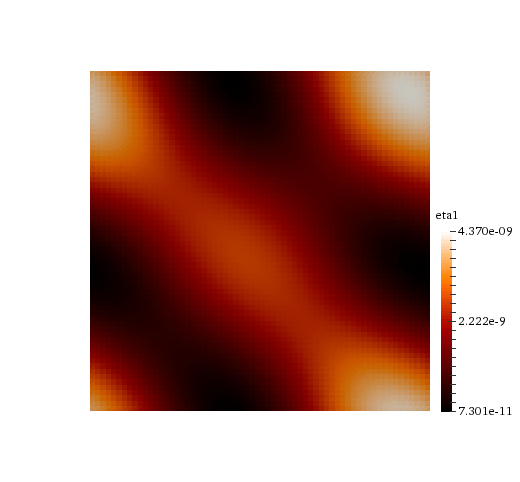
\includegraphics[width=\textwidth,height=\textheight,keepaspectratio,height=\textheight,keepaspectratio]{figures/2_mpet/no_transfer/space/eta1_64.png}
    \caption{$N=64$}
  \end{subfigure}
  \caption{Error magnitude for $\eta_1$ under space refinement at $t=T$ for two-network MPET model with non-interacting fluid networks} \label{fig:bb_no_transfer_eta1}
\end{figure}
\begin{figure}[h!]
  \centering
  \begin{subfigure}[b]{0.24\textwidth}
    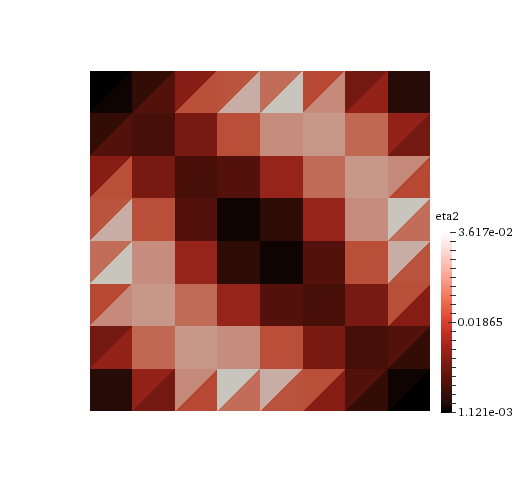
\includegraphics[width=\textwidth,height=\textheight,keepaspectratio,height=\textheight,keepaspectratio]{figures/2_mpet/no_transfer/space/eta2_8.png}
    \caption{$N=8$}
  \end{subfigure}
  \begin{subfigure}[b]{0.24\textwidth}
    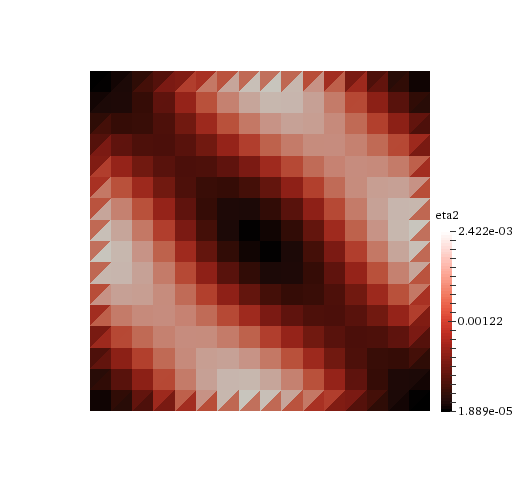
\includegraphics[width=\textwidth,height=\textheight,keepaspectratio,height=\textheight,keepaspectratio]{figures/2_mpet/no_transfer/space/eta2_16.png}
    \caption{$N=16$}
  \end{subfigure}
  \begin{subfigure}[b]{0.24\textwidth}
    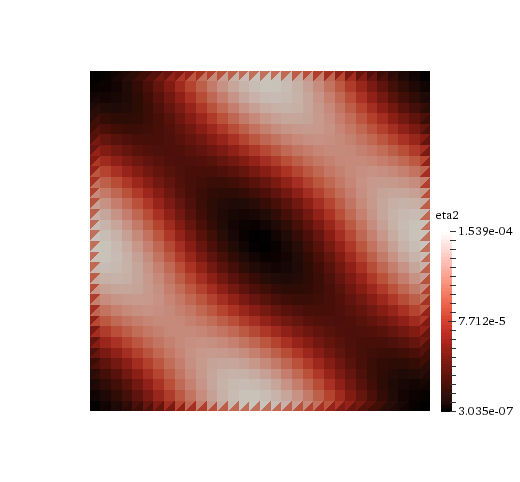
\includegraphics[width=\textwidth,height=\textheight,keepaspectratio,height=\textheight,keepaspectratio]{figures/2_mpet/no_transfer/space/eta2_32.png}
    \caption{$N=32$}
  \end{subfigure}
  \begin{subfigure}[b]{0.24\textwidth}
    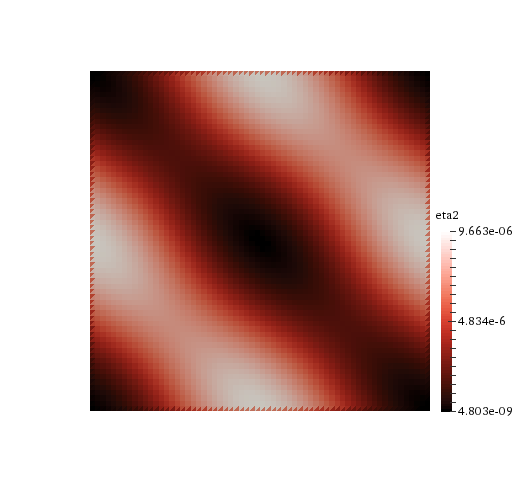
\includegraphics[width=\textwidth,height=\textheight,keepaspectratio,height=\textheight,keepaspectratio]{figures/2_mpet/no_transfer/space/eta2_64.png}
    \caption{$N=64$}
  \end{subfigure}
  \caption{Error magnitude for $\eta_2$ under space refinement at $t=T$ for two-network MPET model with non-interacting fluid networks} \label{fig:bb_no_transfer_eta2}
\end{figure}
\begin{figure}[h!]
  \centering
  \begin{subfigure}[b]{0.24\textwidth}
    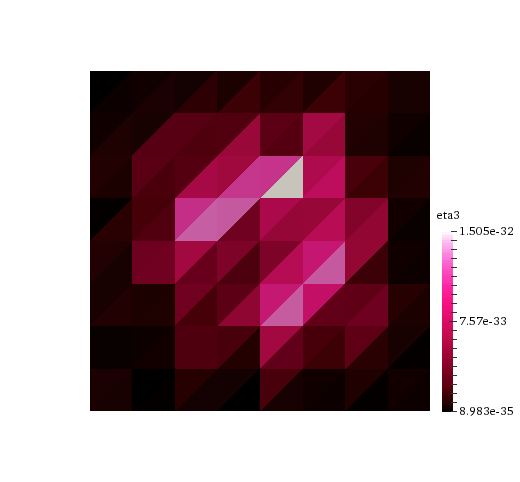
\includegraphics[width=\textwidth,height=\textheight,keepaspectratio,height=\textheight,keepaspectratio]{figures/2_mpet/no_transfer/space/eta3_8.png}
    \caption{$N=8$}
  \end{subfigure}
  \begin{subfigure}[b]{0.24\textwidth}
    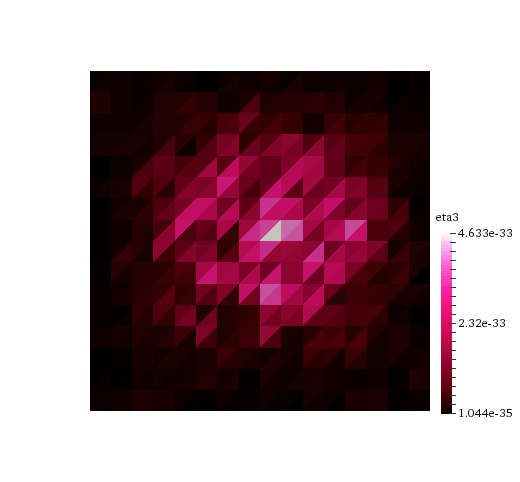
\includegraphics[width=\textwidth,height=\textheight,keepaspectratio,height=\textheight,keepaspectratio]{figures/2_mpet/no_transfer/space/eta3_16.png}
    \caption{$N=16$}
  \end{subfigure}
  \begin{subfigure}[b]{0.24\textwidth}
    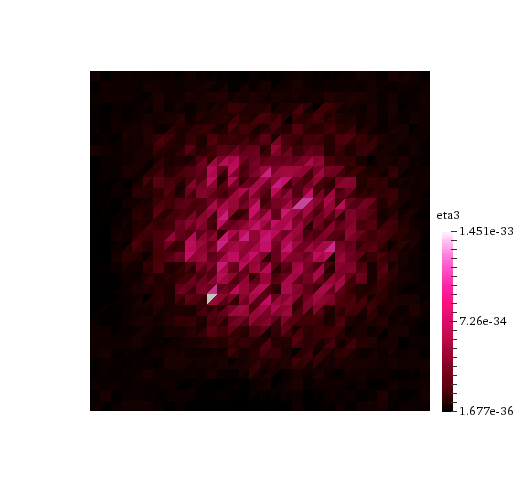
\includegraphics[width=\textwidth,height=\textheight,keepaspectratio,height=\textheight,keepaspectratio]{figures/2_mpet/no_transfer/space/eta3_32.png}
    \caption{$N=32$}
  \end{subfigure}
  \begin{subfigure}[b]{0.24\textwidth}
    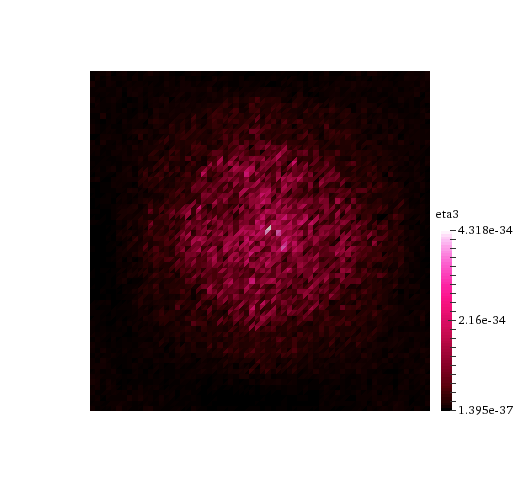
\includegraphics[width=\textwidth,height=\textheight,keepaspectratio,height=\textheight,keepaspectratio]{figures/2_mpet/no_transfer/space/eta3_64.png}
    \caption{$N=64$}
  \end{subfigure}
  \caption{Error magnitude for $\eta_3$ under space refinement at $t=T$ for two-network MPET model with non-interacting fluid networks} \label{fig:bb_no_transfer_eta3}
\end{figure}
\begin{figure}[h!]
  \centering
  \begin{subfigure}[b]{0.24\textwidth}
    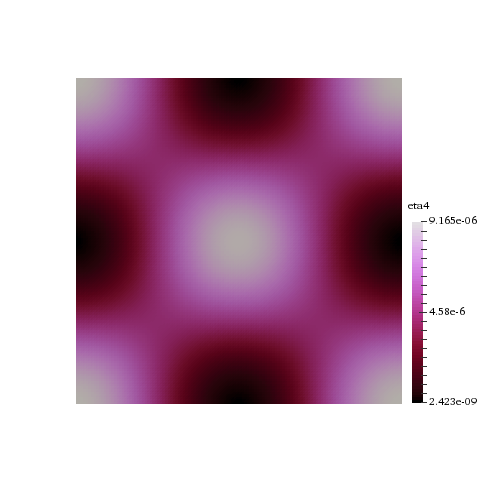
\includegraphics[width=\textwidth,height=\textheight,keepaspectratio,height=\textheight,keepaspectratio]{figures/2_mpet/no_transfer/time/eta4_dt1.png}
    \caption{$\tau=0.01$}
  \end{subfigure}
  \begin{subfigure}[b]{0.24\textwidth}
    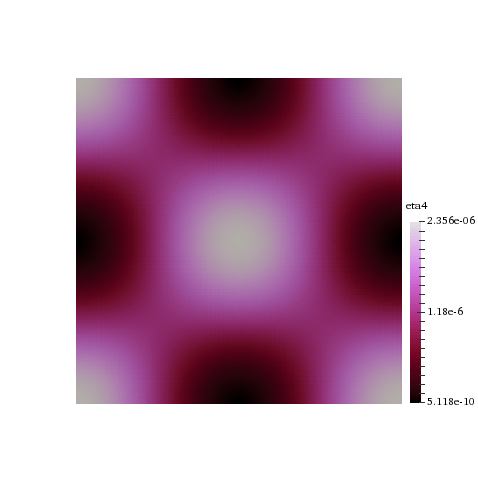
\includegraphics[width=\textwidth,height=\textheight,keepaspectratio,height=\textheight,keepaspectratio]{figures/2_mpet/no_transfer/time/eta4_dt2.png}
    \caption{$\tau=0.005$}
  \end{subfigure}
  \begin{subfigure}[b]{0.24\textwidth}
    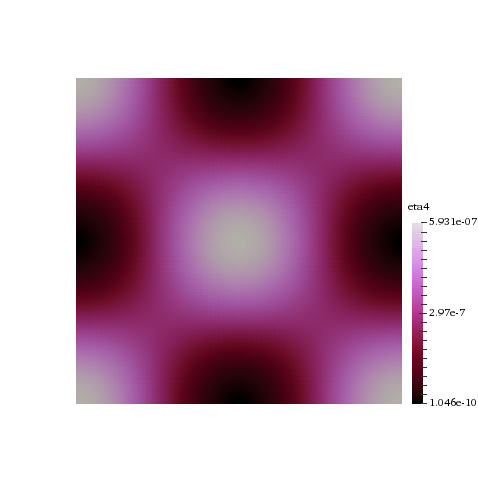
\includegraphics[width=\textwidth,height=\textheight,keepaspectratio,height=\textheight,keepaspectratio]{figures/2_mpet/no_transfer/time/eta4_dt3.png}
    \caption{$\tau=0.0025$}
  \end{subfigure}
  \begin{subfigure}[b]{0.24\textwidth}
    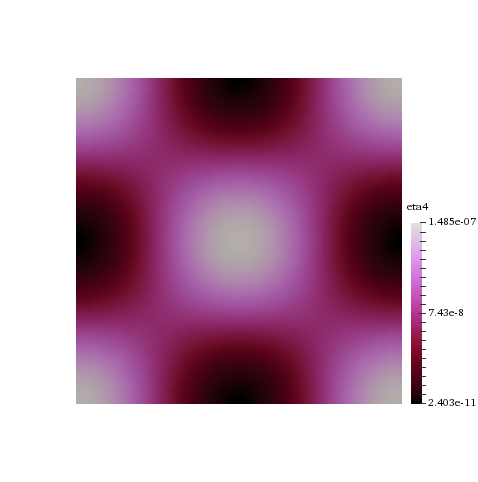
\includegraphics[width=\textwidth,height=\textheight,keepaspectratio,height=\textheight,keepaspectratio]{figures/2_mpet/no_transfer/time/eta4_dt4.png}
    \caption{$\tau=0.00125$}
  \end{subfigure}
  \caption{Error magnitude for $\eta_4$ under time refinement at $t=T$ for two-network MPET model with non-interacting fluid networks} \label{fig:bb_no_transfer_eta4}
\end{figure}
\clearpage
\subsubsection{Two-network poroelasticity: interacting fluid networks} \label{section:num_mpet2_default}
Table \ref{tab:bb_default_transfer_space_error} present the convergence rates for the a priori error estimate for the displacement and the pressures under space refinement with interacting fluid networks where both transfer coefficients are set to 1. The displacement and pressure converge optimally as the mesh is refined. The displacement exhibit the same behavior as with non-interacting fluid networks. This is expected since the displacement is independent of the number of fluid networks. We observe that the a posteriori error estimators yield the same rates as for the Biot model, see table \ref{tab:bb_default_transfer_space_est}. The time estimator $\eta_4$ remains constant under space refinement. The error magnitude for the space estimators $\eta_1$, $\eta_2$ and $\eta_3$ are displayed in figures \ref{fig:bb_default_eta1}, \ref{fig:bb_default_eta2} and \ref{fig:bb_default_eta3}. We observe similar results as with the two network model with non-interacting networks, which indicate that the added transfer terms ($\xi = 1$) do not affect the error magnitude in a significant way.
\\
\\
Table \ref{tab:bb_default_transfer_time_error} displays the convergence rate for the a priori error estimate for the displacement and the pressures under time refinement with interacting fluid networks.  The displacement and the pressure exhibit optimal convergence as the time step is refined. Running simulations with smaller time steps ensure convergence of order 1. The time estimator $\eta_4$ converges optimally, see table \ref{tab:bb_default_transfer_time_est}. Figure \ref{fig:bb_default_eta4} displays the error magnitude for the time estimator $\eta_4$ which is unchanging from the experiment with non-interacting fluid networks. 
\\
\\
\begin{center} 
\centering
\begin{tabular}{c|c|c|c|c|c|c}
$h^{-1}$ & $\|u - u_{h_{\tau}}\|_{H^1}$ & Rate & $\|p_1 - p_{1h_{\tau}}\|_{L^2}$ & Rate & $\|p_2 - p_{2h_{\tau}}\|_{L^2}$ & Rate\\\hline
4  & 3.458e-2 & -     & 2.121e-3 & -     & 2.121e-3 & -     \\
8  & 8.318e-3 & 2.055 & 9.499e-4 & 1.159 & 9.499e-4 & 1.159 \\
16 & 2.038e-3 & 2.029 & 2.699e-4 & 1.816 & 2.699e-4 & 1.816 \\
32 & 5.081e-4 & 2.004 & 6.752e-5 & 1.999 & 6.752e-5 & 1.999 \\
64 & 1.286e-4 & 1.982 & 1.570e-5 & 2.105 & 1.570e-5 & 2.105 \\\hline
Opt. & & 2 & & 2 & & 2
\end{tabular}
\captionof{table}{Error norms and convergence rates for two network MPET model with interacting fluid networks under space refinement, $T=0.1$, $\tau = 5.0$e-5, $\mu=0.5$, $\xi_1 = \xi_2 = 1$, all other parameters set to $1$} \label{tab:bb_default_transfer_space_error}
\end{center}
\mbox{}\\
\begin{center} 
\centering
\begin{tabular}{c|c|c|c|c|c|c|c}
$h^{-1}$ & $\eta_1$ & Rate &  $\eta_2$ & Rate & $\eta_3$ & Rate & $\eta_4$ \\\hline
4  & 9.626e-1 & -     & 5.173e-1 & -     & 1.530e-3 & -     & 4.067e-4 \\
8  & 2.454e-1 & 1.972 & 2.839e-1 & 0.865 & 7.860e-4 & 0.961 & 4.123e-4 \\
16 & 6.167e-2 & 1.992 & 1.462e-1 & 0.958 & 3.961e-4 & 0.988 & 4.133e-4 \\
32 & 1.544e-2 & 1.998 & 7.396e-2 & 0.983 & 1.985e-4 & 0.997 & 4.135e-4 \\
64 & 3.863e-3 & 1.999 & 3.717e-2 & 0.993 & 9.930e-5 & 0.999 & 4.136e-4 \\\hline
Opt. & & 2 & & 1  & & 2 & 
\end{tabular}
\captionof{table}{Convergence rate for a posteriori error estimates for the two network MPET model with interacting fluid networks under space refinement, $T=0.1$, $\tau = 5.0$e-5, $\mu=0.5$, $\xi_1 = \xi_2 = 1$, all other parameters set to $1$} \label{tab:bb_default_transfer_space_est}
\end{center}

\clearpage

\begin{center} 
\centering
\small
\begin{tabular}{c|c|c|c|c|c|c}
$\tau$ & $\|u-u_{h_{\tau}}\|_{H^1}$ & Rate & $\|p_1-p_{1h_{\tau}}\|_{L^2}$ & Rate & $\|p_2-p_{2h_{\tau}}\|_{L^2}$ & Rate \\\hline
0.02   	& 2.912e-3 & -     & 4.503e-3 & -     & 4.503e-3 &  -    \\
0.01   	& 1.258e-3 & 1.210 & 1.936e-3 & 1.218 & 1.936e-3 & 1.218 \\
0.005  	& 5.807e-4 & 1.116 & 8.892e-4 & 1.122 & 8.892e-4 & 1.122 \\
0.0025  & 2.798e-4 & 1.053 & 4.258e-4 & 1.062 & 4.258e-4 & 1.062 \\
0.00125 & 1.392e-4 & 1.007 & 2.093e-4 & 1.025 & 2.093e-4 & 1.025 \\ \hline
Opt. & & 1 & & 1  & & 1
\end{tabular}
\normalsize
\captionof{table}{Error estimates and convergence rates for the two network MPET model with interacting fluid networks under time refinement, $T=1$, $h=1/64$, $\mu=0.5$, $\xi_1 = \xi_2 = 1$, all other parameters set to $1$} \label{tab:bb_default_transfer_time_error}
\end{center}
\mbox{}\\ \\
\begin{center}
\centering
\begin{tabular}{c|c|c|c|c|c}
$\tau$ & $\eta_1$ & $\eta_2$ & $\eta_3$ & $\eta_4$ & Rate\\\hline
0.02    & 2.948e-3 & 1.185e-1 & 1.985e-2 & 3.846e-1 & -    \\
0.01    & 2.947e-3 & 1.190e-1 & 9.930e-3 & 1.948e-1 & 0.981\\
0.005   & 2.947e-3 & 1.192e-1 & 4.965e-3 & 9.806e-2 & 0.991\\
0.0025  & 2.948e-3 & 1.194e-1 & 2.483e-3 & 4.919e-2 & 0.995\\
0.00125 & 2.948e-3 & 1.194e-1 & 1.241e-3 & 2.463e-2 & 0.998\\\hline
Opt. & & & & & 1
\end{tabular}
\captionof{table}{A posteriori error and convergence rates for the Barenblatt-Biot model with interacting fluid networks under time refinement, $T=1$, $h=1/64$, $\mu=0.5$, $\xi_1 = \xi_2 = 1$, all other parameters set to $1$}  \label{tab:bb_default_transfer_time_est}
\end{center}
\mbox{}\\ \\ \\
\begin{figure}[h!]
  \centering
  \begin{subfigure}[b]{0.24\textwidth}
    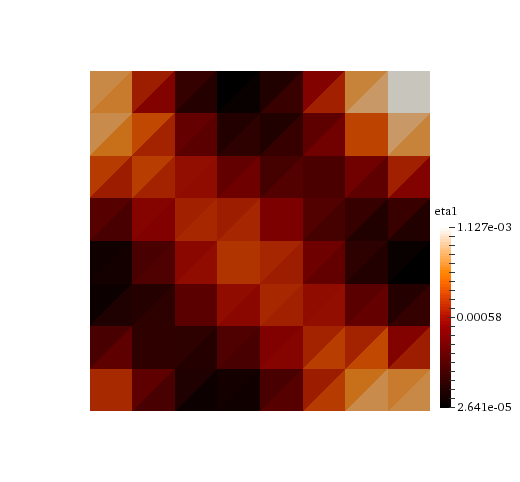
\includegraphics[width=\textwidth,height=\textheight,keepaspectratio,height=\textheight,keepaspectratio]{figures/2_mpet/no_transfer/space/eta1_8.png}
    \caption{$N=8$}
  \end{subfigure}
  \begin{subfigure}[b]{0.24\textwidth}
    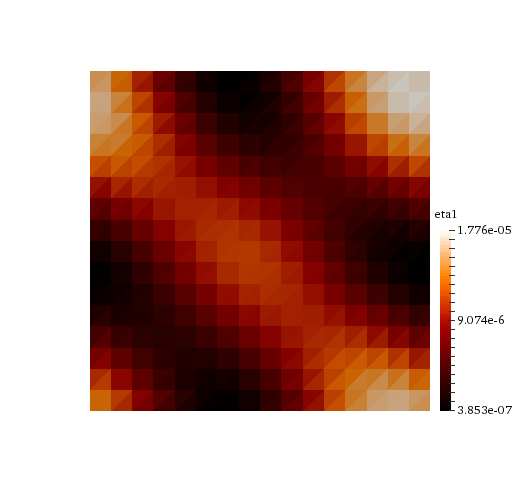
\includegraphics[width=\textwidth,height=\textheight,keepaspectratio,height=\textheight,keepaspectratio]{figures/2_mpet/no_transfer/space/eta1_16.png}
    \caption{$N=16$}
  \end{subfigure}
  \begin{subfigure}[b]{0.24\textwidth}
    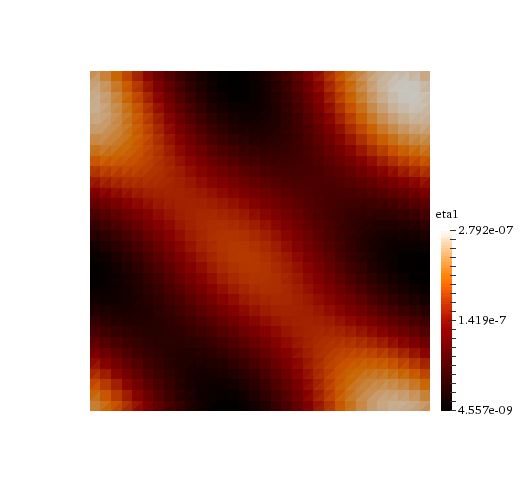
\includegraphics[width=\textwidth,height=\textheight,keepaspectratio,height=\textheight,keepaspectratio]{figures/2_mpet/no_transfer/space/eta1_32.png}
    \caption{$N=32$}
  \end{subfigure}
  \begin{subfigure}[b]{0.24\textwidth}
    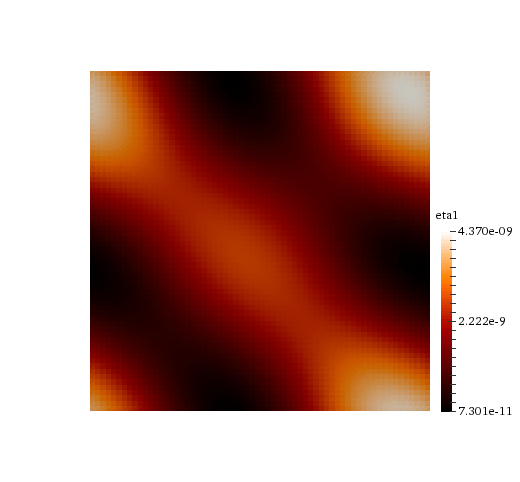
\includegraphics[width=\textwidth,height=\textheight,keepaspectratio,height=\textheight,keepaspectratio]{figures/2_mpet/no_transfer/space/eta1_64.png}
    \caption{$N=64$}
  \end{subfigure}
  \caption{Error magnitude for $\eta_1$ under space refinement at $t=T$ for two-network MPET model with interacting fluid networks} \label{fig:bb_default_eta1}
\end{figure}

\clearpage

\begin{figure}[h!]
  \centering
  \begin{subfigure}[b]{0.24\textwidth}
    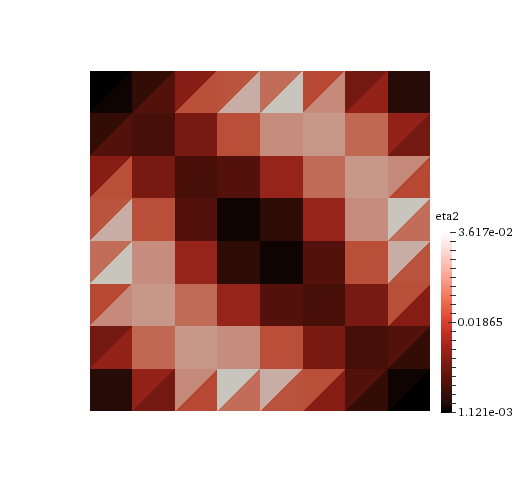
\includegraphics[width=\textwidth,height=\textheight,keepaspectratio,height=\textheight,keepaspectratio]{figures/2_mpet/no_transfer/space/eta2_8.png}
    \caption{$N=8$}
  \end{subfigure}
  \begin{subfigure}[b]{0.24\textwidth}
    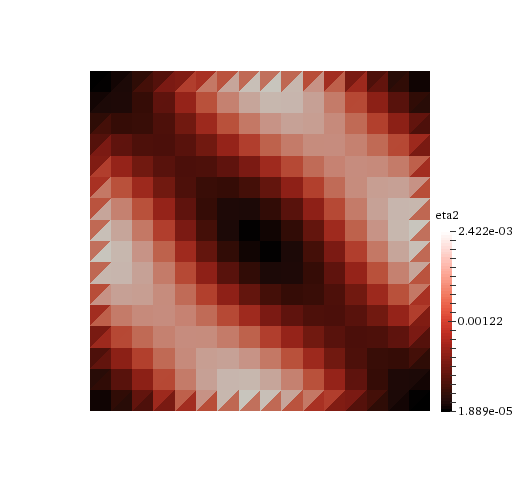
\includegraphics[width=\textwidth,height=\textheight,keepaspectratio,height=\textheight,keepaspectratio]{figures/2_mpet/no_transfer/space/eta2_16.png}
    \caption{$N=16$}
  \end{subfigure}
  \begin{subfigure}[b]{0.24\textwidth}
    \includegraphics[width=\textwidth,height=\textheight,keepaspectratio,height=\textheight,keepaspectratio]{figures/2_mpet/no_transfer/space/eta2_32.png}
    \caption{$N=32$}
  \end{subfigure}
  \begin{subfigure}[b]{0.24\textwidth}
    \includegraphics[width=\textwidth,height=\textheight,keepaspectratio,height=\textheight,keepaspectratio]{figures/2_mpet/no_transfer/space/eta2_64.png}
    \caption{$N=64$}
  \end{subfigure}
  \caption{Error magnitude for $\eta_2$ under space refinement at $t=T$ for two-network MPET model with interacting fluid networks} \label{fig:bb_default_eta2}
\end{figure}
\mbox{}\\ \\
\begin{figure}[h!]
  \centering
  \begin{subfigure}[b]{0.24\textwidth}
    \includegraphics[width=\textwidth,height=\textheight,keepaspectratio,height=\textheight,keepaspectratio]{figures/2_mpet/default/space/eta3_8.png}
    \caption{$N=8$}
  \end{subfigure}
  \begin{subfigure}[b]{0.24\textwidth}
    \includegraphics[width=\textwidth,height=\textheight,keepaspectratio,height=\textheight,keepaspectratio]{figures/2_mpet/default/space/eta3_16.png}
    \caption{$N=16$}
  \end{subfigure}
  \begin{subfigure}[b]{0.24\textwidth}
    \includegraphics[width=\textwidth,height=\textheight,keepaspectratio,height=\textheight,keepaspectratio]{figures/2_mpet/default/space/eta3_32.png}
    \caption{$N=32$}
  \end{subfigure}
  \begin{subfigure}[b]{0.24\textwidth}
    \includegraphics[width=\textwidth,height=\textheight,keepaspectratio,height=\textheight,keepaspectratio]{figures/2_mpet/default/space/eta3_64.png}
    \caption{$N=64$}
  \end{subfigure}
  \caption{Error magnitude for $\eta_3$ under space refinement at $t=T$ for two-network MPET model with interacting fluid networks} \label{fig:bb_default_eta3}
\end{figure}
\mbox{}\\ \\
\begin{figure}[h!]
  \centering
  \begin{subfigure}[b]{0.24\textwidth}
    \includegraphics[width=\textwidth,height=\textheight,keepaspectratio,height=\textheight,keepaspectratio]{figures/2_mpet/default/time/eta4_dt1.png}
    \caption{$\tau=0.01$}
  \end{subfigure}
  \begin{subfigure}[b]{0.24\textwidth}
    \includegraphics[width=\textwidth,height=\textheight,keepaspectratio,height=\textheight,keepaspectratio]{figures/2_mpet/default/time/eta4_dt2.png}
    \caption{$\tau=0.005$}
  \end{subfigure}
  \begin{subfigure}[b]{0.24\textwidth}
    \includegraphics[width=\textwidth,height=\textheight,keepaspectratio,height=\textheight,keepaspectratio]{figures/2_mpet/default/time/eta4_dt3.png}
    \caption{$\tau=0.0025$}
  \end{subfigure}
  \begin{subfigure}[b]{0.24\textwidth}
    \includegraphics[width=\textwidth,height=\textheight,keepaspectratio,height=\textheight,keepaspectratio]{figures/2_mpet/default/time/eta4_dt4.png}
    \caption{$\tau=0.00125$}
  \end{subfigure}
  \caption{Error magnitude for $\eta_4$ under time refinement at $t=T$ for two-network MPET model with interacting fluid networks} \label{fig:bb_default_eta4}
\end{figure}
\clearpage
\subsubsection{Two-network poroelasticity: physiological parameters} \label{section:num_mpet2_bio}
The main interest in using the MPET model is to simulate interacting biological fluids in a physiological setting. Thus, we perform a numerical experiment with two networks on the unit square with physiologically inspired parameters \cite{lee2018}, presented below in table \ref{tab:bb_parameters}. 
\begin{center}
\begin{tabular}{c|c|c}
Parameter & Value(s) & Unit \\\hline
$\alpha_1$  & 0.49 & -\\
$\alpha_2$  & 0.25 & -\\
$\nu$ & 0.499 & -\\
$E$ & 1500 & Pa\\
$c_1$ & $3.9 \cdot 10^{-4}$ & Pa$^{-1}$ \\
$c_2$ & $2.9 \cdot 10^{-4}$ & Pa$^{-1}$ \\
$K_1$ & $1.57 \cdot 10^{-5}$ & mm$^2$ Pa$^{-1}$ s$^{-1}$ \\
$K_2$ & $3.75 \cdot 10^{-2}$ & mm$^2$ Pa$^{-1}$ s$^{-1}$ \\
$\xi_{1}, \xi_{2}$ & 0.0 & Pa$^{-1}$ s$^{-1}$ \\
\end{tabular}
\captionof{table}{Model parameters for the two-network model for physiologically inspired numerical experiment} \label{tab:bb_parameters}
\end{center}
% gives mu = 500.033335556, lamb =  2499666.64444
Table \ref{tab:bb_bio_space_error} present the convergence rates for the a priori error estimate for the displacement and the pressures under space refinement with physiologically inspired parameters. We observe that the convergence rate for the displacement appears to increase as the mesh is refined. The pressures exhibit oscillating behavior. This is known as poroelastic locking, which occurs when the displacement is underestimated when the material is assumed to be incompressible \cite{phillips}. When some parameters are small compared to the others, the numerical approximation may become unreliable. Here, $\lambda \approx 2.499 \cdot 10^6$ and $c, K \leq 3.75 \cdot 10^{-2}$; thus the variation in the size of the parameters is considered to be large. This problem is addressed by Lee et al. \cite{lee2018}, where the proposed solution is to implement a total pressure formulation.  
\\
\\
The quantities $\eta_1$ and $\eta_3$ are approximately $10^6$ times larger compared to the first experiment with non-interacting fluid networks under space refinement. This is illustrated in table \ref{tab:bb_bio_space_est}. The estimator associated with the time error, $\eta_4$ remains constant under space refinement. Since $\eta_1$ and $\eta_3$ are dependent on the size of $\lambda$, we will expect that these quantities increase proportionally with $\lambda$. The quantities $\eta_2$ and $\eta_4$ are approximately $10^{-1}$ times smaller compared to the interactive network case with all parameters set to 2. This is expected as these estimators are dependent on the size of $c$ and $K$. In table \ref{tab:bb_bio_space_est} we observe that $\eta_1$ exhibit a slightly sub-optimal convergence, while $\eta_2$ converges optimally. The quantity $\eta_3$ converges to 1, (similarly to the single network case), that is, one order lower than optimal. The error magnitude for the space estimators $\eta_1$, $\eta_2$ and $\eta_3$ are presented in figures \ref{fig:bb_bio_eta1}, \ref{fig:bb_bio_eta2} and \ref{fig:bb_bio_eta3} respectively. We observe that the quantity detecting the residual error for the displacement under space refinement, $\eta_1$, is much larger than $\eta_3$. Recall that $\eta_3$ could heuristically be described as a measure of the change in the displacement-related spatial residual in time. As mentioned previously, this suggests a further refinement in space. 
\\
\\
Table \ref{tab:bb_bio_time_error} displays the convergence rate for the displacement and the pressures under time refinement, which indicates optimal rates for $u$ and $p_1$. The second pressure term $p_2$ exhibit tendencies of superconvergence. That is, it converges at a higher order than expected \cite{ferreira}. The error quantities $\eta_1$ and $\eta_3$ are approximately $10^6$ times larger compared to the non-interactive network experiment under time refinement, see table \ref{tab:bb_bio_time_est}. As we stated above, this is expected since they depend on the size of $\lambda$. We also observe a slightly sub-optimal convergence for $\eta_4$. $\eta_1$ and $\eta_2$ remains constant under time refinement. This is expected as they are associated with the space error. The quantity $\eta_3$ is also associated with the space error; however, it is a time-incremental version of the $\eta_1$, which results in a time-dependence. This quantity converges to 1 under time refinement. Figure  \ref{fig:bb_bio_eta4} presents the error magnitude for the time estimator $\eta_4$ under time refinement, where the lighter areas display where the error is concentrated. 
\\
\\
\begin{center} 
\centering
\begin{tabular}{c|c|c|c|c|c|c}
$h^{-1}$ & $\|u - u_{h_{\tau}}\|_{H^1}$ & Rate & $\|p_1 - p_{1h_{\tau}}\|_{L^2}$ & Rate & $\|p_2 - p_{2h_{\tau}}\|_{L^2}$ & Rate\\\hline
4  & 8.125e-2 & -     & 5.458e-1 & -     & 5.131e-3 & -     \\
8  & 4.449e-2 & 0.869 & 2.537e-2 & 4.427 & 1.652e-3 & 1.635 \\
16 & 1.854e-2 & 1.263 & 1.303e-2 & 0.962 & 4.495e-4 & 1.878 \\
32 & 5.563e-3 & 1.737 & 1.468e-2 & -0.172 & 1.383e-4 & 1.700 \\
64 & 1.203e-3 & 2.209 & 1.476e-2 & -0.008 & 8.532e-5 & 0.697 \\\hline
Opt. & & 2 & & 2 & & 2
\end{tabular}
\captionof{table}{Error norms and convergence rates for two network MPET model under space refinement, $T=0.1$, $\tau = 5.0$e-5, with physiologically inspired parameters} \label{tab:bb_bio_space_error}
\end{center}
\mbox{}\\ \\ \\
\begin{center} 
\centering
\begin{tabular}{c|c|c|c|c|c|c|c}
$h^{-1}$ & $\eta_1$ & Rate &  $\eta_2$ & Rate & $\eta_3$ & Rate & $\eta_4$ \\\hline
4  & 1.123e+6 & -     & 1.302e-2 & -     & 1.905e+3 & -     & 3.874e-5 \\
8  & 2.830e+5 & 1.989 & 7.381e-3 & 0.819 & 9.651e+2 & 0.981 & 3.966e-5 \\
16 & 7.143e+4 & 1.986 & 3.855e-3 & 0.937 & 4.841e+2 & 0.996 & 3.995e-5 \\
32 & 1.816e+4 & 1.975 & 1.958e-3 & 0.997 & 2.422e+2 & 0.999 & 4.003e-5 \\
64 & 4.634e+3 & 1.971 & 9.854e-4 & 0.991 & 1.211e+2 & 1.000 & 4.005e-5 \\\hline
Opt. & & 2 & & 1  & & 2 & 
\end{tabular}
\captionof{table}{Convergence rate for a posteriori error estimates for two network MPET model under space refinement, $T=0.1$, $\tau = 5.0$e-5, with physiologically inspired parameters} \label{tab:bb_bio_space_est}
\end{center}

\clearpage

\begin{center} 
\centering
\small
\begin{tabular}{c|c|c|c|c|c|c}
$\tau$ & $\|u-u_{h_{\tau}}\|_{H^1}$ & Rate & $\|p_1-p_{1h_{\tau}}\|_{L^2}$ & Rate & $\|p_2-p_{2h_{\tau}}\|_{L^2}$ & Rate \\\hline
0.02   	& 4.602e-5 & -     & 1.704e+2 & -     & 8.891e-3 &  -    \\
0.01   	& 2.300e-5 & 1.001 & 8.492e+1 & 1.005 & 2.258e-3 & 1.977 \\
0.005  	& 1.149e-5 & 1.001 & 4.238e+1 & 1.003 & 5.811e-4 & 1.958 \\
0.0025  & 5.746e-6 & 1.000 & 2.117e+1 & 1.001 & 1.535e-4 & 1.920 \\
0.00125 & 2.873e-6 & 1.000 & 1.058e+1 & 1.001 & 4.251e-5 & 1.853 \\ \hline
Opt. & & 1 & & 1  & & 1
\end{tabular}
\normalsize
\captionof{table}{Error estimates and convergence rates for the two network MPET model with interacting fluid networks under time refinement, $T=1$, $h=1/64$, with physiologically inspired parameters} \label{tab:bb_bio_time_error}
\end{center}
\mbox{} \\ \\ \\ 
\begin{center} 
\centering
\begin{tabular}{c|c|c|c|c|c}
$\tau$ & $\eta_1$ & $\eta_2$ & $\eta_3$ & $\eta_4$ & Rate\\\hline
0.02    & 3.801e+3 & 3.268e-3 & 2.421e+4 & 8.249e-2 & -    \\
0.01    & 3.801e+3 & 3.194e-3 & 1.211e+4 & 2.643e-2 & 1.642\\
0.005   & 3.801e+3 & 3.175e-3 & 6.057e+3 & 1.057e-2 & 1.322\\
0.0025  & 3.801e+3 & 3.171e-3 & 3.029e+3 & 4.905e-3 & 1.108\\
0.00125 & 3.801e+3 & 3.169e-3 & 1.514e+3 & 2.404e-3 & 1.029\\\hline
Opt. & & & & & 1
\end{tabular}
\captionof{table}{A posteriori error and convergence rates for the two network MPET model with interacting fluid networks under time refinement, $T=1$, $h=1/64$, with physiologically inspired parameters} \label{tab:bb_bio_time_est}
\end{center}
\mbox{}\\ \\ \\ \\
\begin{figure}[h!]
  \centering
  \begin{subfigure}[b]{0.24\textwidth}
    \includegraphics[width=\textwidth,height=\textheight,keepaspectratio,height=\textheight,keepaspectratio]{figures/2_mpet/biomedical/space/eta1_8.png}
    \caption{$N=8$}
  \end{subfigure}
  \begin{subfigure}[b]{0.24\textwidth}
    \includegraphics[width=\textwidth,height=\textheight,keepaspectratio,height=\textheight,keepaspectratio]{figures/2_mpet/biomedical/space/eta1_16.png}
    \caption{$N=16$}
  \end{subfigure}
  \begin{subfigure}[b]{0.24\textwidth}
    \includegraphics[width=\textwidth,height=\textheight,keepaspectratio,height=\textheight,keepaspectratio]{figures/2_mpet/biomedical/space/eta1_32.png}
    \caption{$N=32$}
  \end{subfigure}
  \begin{subfigure}[b]{0.24\textwidth}
    \includegraphics[width=\textwidth,height=\textheight,keepaspectratio,height=\textheight,keepaspectratio]{figures/2_mpet/biomedical/space/eta1_64.png}
    \caption{$N=64$}
  \end{subfigure}
  \caption{Error magnitude for $\eta_1$ under space refinement at $t=T$ for two-network MPET model with physiologically inspired parameters} \label{fig:bb_bio_eta1}
\end{figure}

\clearpage

\begin{figure}[h!]
  \centering
  \begin{subfigure}[b]{0.24\textwidth}
    \includegraphics[width=\textwidth,height=\textheight,keepaspectratio,height=\textheight,keepaspectratio]{figures/2_mpet/biomedical/space/eta2_8.png}
    \caption{$N=8$}
  \end{subfigure}
  \begin{subfigure}[b]{0.24\textwidth}
    \includegraphics[width=\textwidth,height=\textheight,keepaspectratio,height=\textheight,keepaspectratio]{figures/2_mpet/biomedical/space/eta2_16.png}
    \caption{$N=16$}
  \end{subfigure}
  \begin{subfigure}[b]{0.24\textwidth}
    \includegraphics[width=\textwidth,height=\textheight,keepaspectratio,height=\textheight,keepaspectratio]{figures/2_mpet/biomedical/space/eta2_32.png}
    \caption{$N=32$}
  \end{subfigure}
  \begin{subfigure}[b]{0.24\textwidth}
    \includegraphics[width=\textwidth,height=\textheight,keepaspectratio,height=\textheight,keepaspectratio]{figures/2_mpet/biomedical/space/eta2_64.png}
    \caption{$N=64$}
  \end{subfigure}
  \caption{Error magnitude for $\eta_2$ under space refinement at $t=T$ for two-network MPET model with physiologically inspired parameters} \label{fig:bb_bio_eta2}
\end{figure}
\mbox{}\\ \\
\begin{figure}[h!]
  \centering
  \begin{subfigure}[b]{0.24\textwidth}
    \includegraphics[width=\textwidth,height=\textheight,keepaspectratio,height=\textheight,keepaspectratio]{figures/2_mpet/biomedical/space/eta3_8.png}
    \caption{$N=8$}
  \end{subfigure}
  \begin{subfigure}[b]{0.24\textwidth}
    \includegraphics[width=\textwidth,height=\textheight,keepaspectratio,height=\textheight,keepaspectratio]{figures/2_mpet/biomedical/space/eta3_16.png}
    \caption{$N=16$}
  \end{subfigure}
  \begin{subfigure}[b]{0.24\textwidth}
    \includegraphics[width=\textwidth,height=\textheight,keepaspectratio,height=\textheight,keepaspectratio]{figures/2_mpet/biomedical/space/eta3_32.png}
    \caption{$N=32$}
  \end{subfigure}
  \begin{subfigure}[b]{0.24\textwidth}
    \includegraphics[width=\textwidth,height=\textheight,keepaspectratio,height=\textheight,keepaspectratio]{figures/2_mpet/biomedical/space/eta3_64.png}
    \caption{$N=64$}
  \end{subfigure}
  \caption{Error magnitude for $\eta_3$ under space refinement at $t=T$ for two-network MPET model with physiologically inspired parameters} \label{fig:bb_bio_eta3}
\end{figure}
\mbox{}\\ \\
\begin{figure}[h!]
  \centering
  \begin{subfigure}[b]{0.24\textwidth}
    \includegraphics[width=\textwidth,height=\textheight,keepaspectratio,height=\textheight,keepaspectratio]{figures/2_mpet/biomedical/time/eta4_dt1.png}
    \caption{$\tau=0.01$}
  \end{subfigure}
  \begin{subfigure}[b]{0.24\textwidth}
    \includegraphics[width=\textwidth,height=\textheight,keepaspectratio,height=\textheight,keepaspectratio]{figures/2_mpet/biomedical/time/eta4_dt2.png}
    \caption{$\tau=0.005$}
  \end{subfigure}
  \begin{subfigure}[b]{0.24\textwidth}
    \includegraphics[width=\textwidth,height=\textheight,keepaspectratio,height=\textheight,keepaspectratio]{figures/2_mpet/biomedical/time/eta4_dt3.png}
    \caption{$\tau=0.0025$}
  \end{subfigure}
  \begin{subfigure}[b]{0.24\textwidth}
    \includegraphics[width=\textwidth,height=\textheight,keepaspectratio,height=\textheight,keepaspectratio]{figures/2_mpet/biomedical/time/eta4_dt4.png}
    \caption{$\tau=0.00125$}
  \end{subfigure}
  \caption{Error magnitude for $\eta_4$ under time refinement at $t=T$ for two-network model with physiologically inspired parameters} \label{fig:bb_bio_eta4}
\end{figure}
\clearpage

\subsection{Four-network poroelasticity} \label{test_mpet4}
As stated in the introduction, the primary motivation in using the MPET equations is to use them to model fluid transportation in the brain. In light of this, it is essential to be able to control the error on complex geometries. Thus, we present the a posteriori error magnitudes for a four-network MPET model on a mouse brain mesh, see figure \ref{fig:brain_mesh}. These experiments as purely meant as a demonstration of how the a posteriori error estimators will work on a geometry different from the unit square. In addition, the experiment implements the a posteriori error estimates derived for the two network poroelasticity model in chapter \ref{chap:error}, however, extended to four networks which demonstrates that the analytic results do not depend on the network number. 
\\
\\ 
For the four-network poroelasticity model we use the following manufactured solution,
\begin{align*}
u_e = & \, \left(\cos(\pi x)\sin(\pi y)\sin(\pi t), \, \sin( \pi x)\cos(\pi y)\sin(\pi t)\right) \\
p_{1_e} = & = p_{2_e} = p_{3_e} = p_{4_e} \,\sin(\pi x) \sin(\pi y)\sin(2\pi t)  
\end{align*}
We consider the entire boundary to be under clamped conditions with Dirichlet data given by the method of manufactured solution for simplicity. It is important to point out that these boundary conditions are not biophysical, but merely prescribed as a demonstration. Clamped boundary conditions are considered much more accessible to implement than the more comprehensive boundary conditions presented in, e.g. \cite{vardakis}. 
\\
\begin{figure}[h!]
\centering
  \includegraphics[scale=0.5]{figures/4_mpet/biomedical/brain_mesh.png}
  \caption[Caption for LOF]{Mouse brain mesh\footnotemark{} with 39409 cells }
  \label{fig:brain_mesh}
\end{figure}
\footnotetext{   \textcopyright Janis Grobovs, Alexandra Diem and the Allen Mouse Brain Atlas}
\mbox{}\\
The estimator associated with the displacement-related spatial residual under uniform space refinement is displayed in figure \ref{fig:mpet4_eta1}. Only one uniform spatial refinement was performed, as this is a computationally expensive procedure. The estimator describing the pressure-related spatial residual are presented in figures \ref{fig:mpet4_eta2_p1}, \ref{fig:mpet4_eta2_p2}, \ref{fig:mpet4_eta2_p3} and \ref{fig:mpet4_eta2_p4} for the four pressure components, respectively. The first pressure term $p_1$ behaves differently compared to the three other components. That is $p_2$, $p_3$ and $p_4$ exhibit larger concentration of error compared to $p_1$. This suggests that an adaptive refinement process should target $p_2$, $p_3$ and $p_4$. Figure \ref{fig:mpet4_eta3} displays the estimator that measures the change in the displacement-related spatial residual in time. We observe that this estimator yields minimal errors, which suggests that a smaller time step is not necessary to ensure a better refinement in space. The time estimator for each pressure component under time refinement is presented in figure \ref{fig:mpet4_eta4}. Each pressure component exhibits similar error concentrations under time refinement, where we observe that the error decreases as the time step decreases. One important feature of the error estimates is to be able to identify the areas where the error is high; this becomes clearer as we refine uniformly. That is, the resolution increases and we are consequently able to locate the specific areas in need of refinement. This experiment demonstrates how the error is distributed on a complex geometry for each error component. 
\begin{figure}[h!]
  \centering
  \begin{subfigure}[b]{0.49\textwidth}
    \includegraphics[width=\textwidth,height=\textheight,keepaspectratio,height=\textheight,keepaspectratio]{figures/4_mpet/biomedical/space/eta1_1.png}
    \caption{39409 mesh cells}
  \end{subfigure}
  \begin{subfigure}[b]{0.49\textwidth}
    \includegraphics[width=\textwidth,height=\textheight,keepaspectratio,height=\textheight,keepaspectratio]{figures/4_mpet/biomedical/space/eta1_2.png}
    \caption{157636 mesh cells}
  \end{subfigure}
  \caption{Error magnitude for $\eta_1$ under uniform space refinement at $t=T$ for four-network MPET model with physiologically inspired parameters on brain mesh} \label{fig:mpet4_eta1}
\end{figure}


\begin{figure}[h!]
  \centering
  \begin{subfigure}[b]{0.49\textwidth}
    \includegraphics[width=\textwidth,height=\textheight,keepaspectratio,height=\textheight,keepaspectratio]{figures/4_mpet/biomedical/space/eta2_p1_1.png}
    \caption{39409 mesh cells}
  \end{subfigure}
  \begin{subfigure}[b]{0.49\textwidth}
    \includegraphics[width=\textwidth,height=\textheight,keepaspectratio,height=\textheight,keepaspectratio]{figures/4_mpet/biomedical/space/eta2_p1_2.png}
    \caption{157636 mesh cells}
  \end{subfigure}
  \caption{Error magnitude for $\eta_2$ associated with the pressure $p_1$ under uniform space refinement at $t=T$ for four-network MPET model with physiologically inspired parameters on brain mesh} \label{fig:mpet4_eta2_p1}
\end{figure}

\begin{figure}[h!]
  \centering
    \begin{subfigure}[b]{0.49\textwidth}
    \includegraphics[width=\textwidth,height=\textheight,keepaspectratio,height=\textheight,keepaspectratio]{figures/4_mpet/biomedical/space/eta2_p2_1.png}
    \caption{39409 mesh cells}
  \end{subfigure}
  \begin{subfigure}[b]{0.49\textwidth}
    \includegraphics[width=\textwidth,height=\textheight,keepaspectratio,height=\textheight,keepaspectratio]{figures/4_mpet/biomedical/space/eta2_p2_2.png}
    \caption{157636 mesh cells}
  \end{subfigure}
  \caption{Error magnitude for $\eta_2$ associated with the pressure $p_2$ under uniform space refinement at $t=T$ for four-network MPET model with physiologically inspired parameters on brain mesh} \label{fig:mpet4_eta2_p2}
\end{figure}

\begin{figure}[h!]
  \centering
    \begin{subfigure}[b]{0.49\textwidth}
    \includegraphics[width=\textwidth,height=\textheight,keepaspectratio,height=\textheight,keepaspectratio]{figures/4_mpet/biomedical/space/eta2_p3_1.png}
    \caption{39409 mesh cells}
  \end{subfigure}
  \begin{subfigure}[b]{0.49\textwidth}
    \includegraphics[width=\textwidth,height=\textheight,keepaspectratio,height=\textheight,keepaspectratio]{figures/4_mpet/biomedical/space/eta2_p3_2.png}
    \caption{157636 mesh cells}
  \end{subfigure}
  \caption{Error magnitude for $\eta_2$ associated with the pressure $p_3$ under uniform space refinement at $t=T$ for four-network MPET model with physiologically inspired parameters on brain mesh} \label{fig:mpet4_eta2_p3}
\end{figure}

\begin{figure}[h!]
  \centering
    \begin{subfigure}[b]{0.49\textwidth}
    \includegraphics[width=\textwidth,height=\textheight,keepaspectratio,height=\textheight,keepaspectratio]{figures/4_mpet/biomedical/space/eta2_p4_1.png}
    \caption{39409 mesh cells}
  \end{subfigure}
  \begin{subfigure}[b]{0.49\textwidth}
    \includegraphics[width=\textwidth,height=\textheight,keepaspectratio,height=\textheight,keepaspectratio]{figures/4_mpet/biomedical/space/eta2_p4_2.png}
    \caption{157636 mesh cells}
  \end{subfigure}
  \caption{Error magnitude for $\eta_2$ associated with the pressure $p_4$ under uniform space refinement at $t=T$ for four-network MPET model with physiologically inspired parameters on brain mesh} \label{fig:mpet4_eta2_p4}
\end{figure}


\begin{figure}[h!]
  \centering
  \centering
    \begin{subfigure}[b]{0.49\textwidth}
    \includegraphics[width=\textwidth,height=\textheight,keepaspectratio,height=\textheight,keepaspectratio]{figures/4_mpet/biomedical/space/eta3_1.png}
    \caption{39409 mesh cells}
  \end{subfigure}
  \begin{subfigure}[b]{0.49\textwidth}
    \includegraphics[width=\textwidth,height=\textheight,keepaspectratio,height=\textheight,keepaspectratio]{figures/4_mpet/biomedical/space/eta3_2.png}
    \caption{157636 mesh cells}
  \end{subfigure}
  \caption{Error magnitude for $\eta_3$ under uniform space refinement at $t=T$ for four-network MPET model with physiologically inspired parameters on a brain mesh} \label{fig:mpet4_eta3}
\end{figure}

\begin{figure}[h!]
  \centering
  \begin{subfigure}[b]{0.24\textwidth}
    \includegraphics[width=\textwidth,height=\textheight,keepaspectratio,height=\textheight,keepaspectratio]{figures/4_mpet/biomedical/time/eta4_p1_dt1.png}
    \caption{$p_1$, $\tau=0.01$}
  \end{subfigure}
  \begin{subfigure}[b]{0.24\textwidth}
    \includegraphics[width=\textwidth,height=\textheight,keepaspectratio,height=\textheight,keepaspectratio]{figures/4_mpet/biomedical/time/eta4_p1_dt2.png}
    \caption{$p_1$, $\tau=0.005$}
  \end{subfigure}
  \begin{subfigure}[b]{0.24\textwidth}
    \includegraphics[width=\textwidth,height=\textheight,keepaspectratio,height=\textheight,keepaspectratio]{figures/4_mpet/biomedical/time/eta4_p1_dt3.png}
    \caption{$p_1$, $\tau=0.0025$}
  \end{subfigure}
  \begin{subfigure}[b]{0.24\textwidth}
    \includegraphics[width=\textwidth,height=\textheight,keepaspectratio,height=\textheight,keepaspectratio]{figures/4_mpet/biomedical/time/eta4_p1_dt4.png}
    \caption{$p_1$, $\tau=0.00125$}
  \end{subfigure}
  \begin{subfigure}[b]{0.24\textwidth}
    \includegraphics[width=\textwidth,height=\textheight,keepaspectratio,height=\textheight,keepaspectratio]{figures/4_mpet/biomedical/time/eta4_p2_dt1.png}
    \caption{$p_2$, $\tau=0.01$}
  \end{subfigure}
  \begin{subfigure}[b]{0.24\textwidth}
    \includegraphics[width=\textwidth,height=\textheight,keepaspectratio,height=\textheight,keepaspectratio]{figures/4_mpet/biomedical/time/eta4_p2_dt2.png}
    \caption{$p_2$, $\tau=0.005$}
  \end{subfigure}
  \begin{subfigure}[b]{0.2\textwidth}
    \includegraphics[width=\textwidth,height=\textheight,keepaspectratio,height=\textheight,keepaspectratio]{figures/4_mpet/biomedical/time/eta4_p2_dt3.png}
    \caption{$p_2$, $\tau=0.0025$}
  \end{subfigure}
  \begin{subfigure}[b]{0.24\textwidth}
    \includegraphics[width=\textwidth,height=\textheight,keepaspectratio,height=\textheight,keepaspectratio]{figures/4_mpet/biomedical/time/eta4_p2_dt4.png}
    \caption{$p_2$, $\tau=0.00125$}
  \end{subfigure}
  \begin{subfigure}[b]{0.24\textwidth}
    \includegraphics[width=\textwidth,height=\textheight,keepaspectratio,height=\textheight,keepaspectratio]{figures/4_mpet/biomedical/time/eta4_p3_dt1.png}
    \caption{$p_3$, $\tau=0.01$}
  \end{subfigure}
  \begin{subfigure}[b]{0.24\textwidth}
    \includegraphics[width=\textwidth,height=\textheight,keepaspectratio,height=\textheight,keepaspectratio]{figures/4_mpet/biomedical/time/eta4_p3_dt2.png}
    \caption{$p_3$, $\tau=0.005$}
  \end{subfigure}
  \begin{subfigure}[b]{0.24\textwidth}
    \includegraphics[width=\textwidth,height=\textheight,keepaspectratio,height=\textheight,keepaspectratio]{figures/4_mpet/biomedical/time/eta4_p3_dt3.png}
    \caption{$p_3$, $\tau=0.0025$}
  \end{subfigure}
  \begin{subfigure}[b]{0.24\textwidth}
    \includegraphics[width=\textwidth,height=\textheight,keepaspectratio,height=\textheight,keepaspectratio]{figures/4_mpet/biomedical/time/eta4_p3_dt4.png}
    \caption{$p_3$, $\tau=0.00125$}
  \end{subfigure}

  \begin{subfigure}[b]{0.24\textwidth}
    \includegraphics[width=\textwidth,height=\textheight,keepaspectratio,height=\textheight,keepaspectratio]{figures/4_mpet/biomedical/time/eta4_p4_dt1.png}
    \caption{$p_4$, $\tau=0.01$}
  \end{subfigure}
  \begin{subfigure}[b]{0.24\textwidth}
    \includegraphics[width=\textwidth,height=\textheight,keepaspectratio,height=\textheight,keepaspectratio]{figures/4_mpet/biomedical/time/eta4_p4_dt2.png}
    \caption{$p_4$, $\tau=0.005$}
  \end{subfigure}
  \begin{subfigure}[b]{0.24\textwidth}
    \includegraphics[width=\textwidth,height=\textheight,keepaspectratio,height=\textheight,keepaspectratio]{figures/4_mpet/biomedical/time/eta4_p4_dt3.png}
    \caption{$p_4$, $\tau=0.0025$}
  \end{subfigure}
  \begin{subfigure}[b]{0.24\textwidth}
    \includegraphics[width=\textwidth,height=\textheight,keepaspectratio,height=\textheight,keepaspectratio]{figures/4_mpet/biomedical/time/eta4_p4_dt4.png}
    \caption{$p_4$, $\tau=0.00125$}
  \end{subfigure}
  \begin{subfigure}[b]{0.5\textwidth}
    \includegraphics[width=\textwidth,height=\textheight,keepaspectratio,height=\textheight,keepaspectratio]{figures/4_mpet/biomedical/time/eta4_range.png}
  \end{subfigure}
  \caption{Error magnitude for $\eta_4$ associated with pressure terms $p_1$, $p_2$, $p_3$ and $p_4$ (in order) under time refinement at $t=T$ for four-network model with physiologically inspired parameters} \label{fig:mpet4_eta4}
\end{figure}

	\chapter{Discussion and conclusions}
\label{chap:discussion}
This thesis has studied residual-based a posteriori error estimation for the two-network poroelasticity model (i.e.~Barenblatt-Biot), with the main contribution presented in Theorem \ref{theorem}. This result gives the derivation of the a posteriori error estimates for the quasi-static Barenblatt-Biot model. The Barenblatt-Biot model is the simplest form for the generalized equations of poroelasticity (MPET) consisting of more than one network. From an application point of view, MPET models have been used for some time in geomechanics to model complex strata such as highly fissured reservoirs. Such structures are characterized by multiple fluid networks having distinct permeabilities, and porosities \cite{bai,Barenblatt1960,Barenblatt1963,Aifantis1982,Aifantis1984}. Recently, the flexibility offered by the MPET equations in modeling multiple permeable and porous networks has attracted the attention of communities working at the intersection of clinical application, applied mathematics, and biomedical engineering. In this context the simplest systems typically model an organ, e.g.~the brain, using four distinct fluid networks: arterial blood, capillary blood, venous blood, and an interstitial fluid or, in the brain, a combination of interstitial and cerebrospinal fluid \cite{vardakis}. 
\\
\\
Despite the advantages offered by the MPET model, such as accounting for several interacting fluid networks, the application of numerical methods within a complex tissue, such as the brain, faces additional challenges. Such challenges include multiple loading modes, compliant mechanical response, and regional variations in mechanical parameters, among others \cite{goriely}. Moreover, uncertainties in data acquisition can further obfuscate patient-specific simulations based on errors in parameter estimation such as medical imaging techniques. These practical concerns can lead to spatial and temporal errors in numerical simulations used to assist clinicians in patient diagnosis, or in computational models designed to test prominent clinical conjectures such as the glymphatic hypothesis \cite{iliff}. Thus, it is essential to control and potentially minimize the spatial and temporal errors.  
\\
\\
To improve a numerical solution, one must refine the spatial mesh in addition to the temporal interval of interest. In practice, a posteriori error estimates are often employed to refine in both space and time intelligently; one seeks to refine only in areas where the error estimators are large relative to the spatial and temporal discretization levels. Such a strategy can enhance the performance of numerical solvers as spatial refinement increases the size of the linear system to be solved, while time refinement increases the number of solution steps needed to deduce numerical results over the temporal interval. In order to explore the efficacy of the a posteriori estimates, numerical experiments, using the method of manufactured solutions, are put forth in section \ref{section:num_mpet2_default}. Due to the clinical motivation, and future applications for the work, the method of manufactured solutions is also employed on a mesh of a parenchymal slice of the mouse brain in section \ref{test_mpet4} using four fluid networks.  The mechanical parameters selected in the mouse brain test-case model correspond to those referenced in the context of clinical application \cite{vardakis,lee}. The boundary conditions considered, however, are purely clamped conditions; such boundary conditions are not physiological but are straightforward to implement. Nevertheless, this type of test offers some insight into the behavior of the estimators on geometries relevant to the application area. Clinical boundary conditions are more complex and require additional information, such as the production rate of cerebrospinal fluid in the ventricles \cite{guo,vardakis}, and are outside the scope of the current work.
%We have derived a posteriori error estimates 
%The main contribution of this thesis is given in Theorem (?) and is the derivation of the a posteriori estimates for the quasi-static Biot-Barenblatt model.  %The derivation is motivated by a similar approach for Biot's equation having its foundations in %
%based on 
%the work of Ern and Meunier \cite{meunier}. 
\\
\\
A posteriori error analysis for Biot's equation has been discussed in \cite{meunier, riedlbeck}; an a priori analysis can be found in \cite{murad1, murad2, murad3}. For the time-independent case, Nordbotten et al. have derived an a posteriori error estimator \cite{nordbotten}. This thesis has derived a posteriori error estimates for the quasi-static two-network case, i.e. the Barenblatt-Biot model. The derivation of our result, Theorem \ref{theorem}, is motivated by the work of Ern and Meunier \cite{meunier} for the quasi-static Biot equation. The primary differences between our result, and that of Ern and Meunier \cite{meunier}, are the addition of a second mass balance equation, and corresponding transfer terms, in extending to the two-network model. The extension is facilitated by in the analysis by augmenting the Sobolev norm, defined on the pressure space, to a norm including the effect of the transfer terms; this new norm is denoted by $\hat{d}$. The form of the arguments of Theorem \ref{theorem} suggest that extension to the case of four fluid networks is straightforward; as such, the Biot-Barenblatt model is the primary extension of concern, and we assign the full extension to the general multi-network case to future work. The remainder of this section offers additional detail for each fundamental component of the work; section \ref{section:a_posteriori} describes the a posteriori estimates and the extension to the two-network case, section \ref{section:mpet_numerical_res} the numerical tests for the two-network and the four network case, section \ref{section:conclusion} offers concluding thoughts, and section \ref{section:further_work} outlines some limitations of the model and future work. 

%We have performed numerical experiments to evaluate the estimates, where we performed a simple experiment and a physiologically inspired experiment on the unit square with two networks. In addition, we presented a purely computational experiment with a four-network MPET model using a brain mesh and physiologically relevant parameters. For this experiment, the analysis of the a posteriori error estimates was not presented as it is a simple extension of the two-network model. 

%A posteriori error analysis for MPET with one network has been covered in \cite{meunier, riedlbeck} and an a priori error analysis can be found in \cite{murad1, murad2, murad3}. Nordbotten et al. have derived an a posteriori error estimator for the static two-network case \cite{nordbotten}. This thesis has derived a posteriori error estimates for the quasi-static two-network case, i.e. the Barenblatt-Biot model. 

\section{A posteriori error estimates} \label{section:a_posteriori}
The a posteriori error estimates for the two-network MPET model is an extension from the one-network MPET model which has been derived in \cite{meunier}. The in-detail analysis and derivation for the one-network model can be found in section \ref{section:error_biot} where in particular the proof structure in section \ref{biot_proof_struc} forms the basis for the extension to the two-network model. The primary differences between our result, and that of Ern and Meunier \cite{meunier}, are the addition of a second mass balance equation, and corresponding transfer terms, in extending to the two-network model. Assuming non-interacting fluid networks will only differ from the one-network model in the added mass balance equation. The derivation of the a posteriori error estimate for MPET with non-interacting fluid networks will thus follow the same arguments as in \cite{meunier} and has been outlined in section \ref{bb:case1_res_err}. In the case of interacting fluid networks, the extension is facilitated by in the analysis by augmenting the Sobolev norm to a new norm denoted by $\hat{d}$ defined in equation \eqref{d_hat_norm}. This norm is defined on the pressure space to include the effect of the transfer terms. The main result containing the upper bound and lower bound on the error for the two-network MPET model is presented in Theorem \ref{theorem}. This result depends on the stability of the continuous problem. In order to arrive at the upper bound, all the equations are summed to get a total error on the left-hand side and the residual-terms on the right-hand side, see equation \eqref{bb:add_forms}. Similarly, for the lower bound, see equations \eqref{mpet2_low_bd1}-\eqref{mpet2_low_bd2} we arrive at one bound for the first equation \eqref{math_model:mpet2_u} and one bound for the pressure terms in \eqref{math_model:mpet2_p1}-\eqref{math_model:mpet2_p2} in section \ref{section:mpet}. Thus, the extension of the a posteriori error estimate to an arbitrary number of networks will not need any additional analysis but should be able to follow the same arguments as presented in this work. 
\\
\\
The a posteriori error estimates for the two-network MPET model was derived in chapter \ref{chap:error} where the main results were presented in Proposition \ref{prop} and Theorem \ref{theorem}. We derived four different estimators for the upper bound of the error, denoted as $\eta_1$, $\eta_2$, $\eta_3$ and $\eta_4$. These estimators provide different indications on how the error behaves in time and space, where $\eta_1$, $\eta_2$ and $\eta_3$ are space estimators and $\eta_4$ is a time estimator. The estimator $\eta_1$ is associated with the spatial residual of the displacement $u$, and $\eta_2$ is associated with the spatial residual of the pressure $p$. $\eta_3$ is defined as the time incremental version of $\eta_1$ and will predict how time may affect the residual of the displacement under space refinement. In other words, $\eta_3$ heuristically measures the change in the displacement-related spatial residual in time. Thus, if $\eta_1$ is small compared to $\eta_3$ indicates further refinement in time. Conversely, if $\eta_3$ is small compared to $\eta_1$, indicates further refinement in space. The magnitude of these two estimators provides the necessary information on \textit{how} to refine. $\eta_4$ is a time estimator associated with the pressure, predicting how time will affect the pressure-solution.
\\
\\
In order to derive the estimates, we assumed that the exact solution of the unknowns was smooth in time and space. This may be a limitation in some applications, e.g. fracture reservoirs in geomechanical engineering which may include solutions with discontinuities. However, in biomedical applications, we do not encounter this specific type of problem. The a posteriori error estimators constructed for the MPET model will naturally depend on the model parameters. That is, if a parameter changes, the estimators associated with that parameters also changes. This was demonstrated in the experiment executed with physiologically relevant parameters in section  \ref{test_bb} where we observed a proportional relationship between the estimators and their associated model parameters.


\section{Numerical results} \label{section:mpet_numerical_res}
This section presents the main results from the numerical experiments outlined in chapter \ref{chap:experiments}, which included the evaluation of the a posteriori error estimates for the two-network and four-network poroelasticity model. 

\subsection{MPET: 2 networks}
For the two-network poroelasticity model with interacting fluid networks, using default parameters all set to 1 yields optimal convergence rates as expected from the a priori error estimates presented in section  \ref{section:a_priori}. That is, a $H^1$-rate and a $L^2$-rate of second order for the displacement and the pressures, respectively under space refinement, and of first order under time refinement, cf. table \ref{tab:bb_default_transfer_space_error} and table \ref{tab:bb_default_transfer_time_error}. The a posteriori error estimates converge optimally under time refinement, cf. table \ref{tab:bb_default_transfer_time_est}. However, under space refinement, the estimator predicting the change in the displacement-related spatial residual in time converges at an order lower than expected from the analysis in \cite{meunier}, cf. table \ref{tab:bb_default_transfer_space_est}. The potential of the a posteriori error estimates is demonstrated in cf. figures \ref{fig:bb_default_eta1}, \ref{fig:bb_default_eta2}, \ref{fig:bb_default_eta3} and \ref{fig:bb_default_eta4} as the error magnitudes indicate where the error is concentrated for the residual related to the displacement and the pressure under time and space refinement. 
\\
\\
Applying physiologically inspired parameters on the two-network poroelasticity model with interacting fluid networks yields an increasing convergence rate for the displacement and oscillating behavior for the pressure under spatial refinement, cf. table \ref{tab:bb_bio_space_error}. This computational behavior is known as "locking" and occurs when the displacement is underestimated due to large variations in the size of the model parameters. This is a well-known problem when implementing a two-field discretization, and a proposed solution is to implement e.g. the total pressure formulation presented in \cite{lee, lee2018} and the stabilization technique suggested in \cite{rodrigo}. The a posteriori estimates derived in this work will detect if locking occurs, which is demonstrated by a proportional relationship between the estimates and their associated model parameter, cf. table \ref{tab:bb_bio_space_est} and \ref{tab:bb_bio_time_est}.

\subsection{MPET: 4 networks}
The motivation behind using the MPET equations is to simulate fluid transportation in the brain. In light of this, it is important to be able to control the error on complex geometries such as a brain mesh. Thus, we presented a posteriori error magnitudes for a four-network MPET model on a mouse brain mesh in section \ref{test_mpet4}. The experiment implements the a posteriori error estimates derived for the two network poroelasticity model in chapter \ref{chap:error} extended to four networks. This shows that the analytic results do not depend on the network number. The experiment used simplified boundary conditions, which are not considered physiological. Thus, we are unable to view how the estimators may detect high feature variation in the various parts of the brain. 
\\
\\
Applying physiologically inspired parameters on the four-network poroelasticity model on a brain mesh yields similar results to the two-network model. This was expected, as the only difference between the two experiments was the two additional pressure-terms. We only performed one uniform space refinement, as this is a computationally expensive procedure on a complex geometry, which ratifies the goal of using the a posteriori error estimates for adaptive refinement in this application framework.


\section{Conclusions} \label{section:conclusion}
A posteriori error estimates provide insight on how to intelligently refine in time and space. The goal of applying the a posteriori error estimates is to be able to control the error and refine in the areas where it is needed. Uniform refinement is computationally expensive, whereas adaptive refinement offers a way to decrease the error while maintaining a minimal number of grid points. The a posteriori error estimates are a prerequisite to performing adaptive refinement as they will predict how the error behaves on each mesh cell. The main contribution in this thesis is the derivation of residual-based a posteriori estimates for the quasi-static Barenblatt-Biot model, which is the simplest form for the generalized equations of poroelasticity (MPET) consisting of more than one network. The potential of the estimators has been demonstrated using the technique of manufactured solutions and a poroelasticity benchmark. The estimators yield upper bounds on the error, which included space, time and data estimators. Numerical experiments corroborate the theoretical results. The presented a posteriori error estimates can be extended to the MPET model with an arbitrary number of networks, which was demonstrated with a computational experiment using four networks on a brain mesh.

\section{Further work} \label{section:further_work}
We have derived a posteriori error estimates for the multiple network poroelasticity model with two networks; however, analysis for the general MPET equations with an arbitrary number of networks is desirable.
\\
\\
We encountered the issue of locking when using standard mixed finite element discretization in a nearly incompressible case. An optimal discretization technique is a prerequisite to ensure an optimal a posteriori error estimate, and we suggest implementing an extension to mixed methods and derive the estimators subsequently to ensure robustness. 
\\
\\
The present work can be extended to the use of time-dependent meshes and adaptive simulations using the a posteriori error estimators to evaluate performance in terms of accuracy, precision, and efficiency. In addition, we suggest applying different error estimation techniques, e.g. goal-oriented, hierarchical, H(div)-lifting. 
\\
\\
We also suggest implementing a physiologically relevant test case including boundary conditions, model parameters, and exact solutions, as we believe the a posteriori error estimates may detect high feature contrasts in the various parts of the brain; this is valuable for future biomedical simulations. 
    %\chapter{The First Appendix}
\label{sec:first-app} 
    \backmatter         % Folios in Arabic numerals, unnumbered chapters
    \printbibliography
\end{document}